% Capitolul 5: Volatilitate condiționată: ARCH și GARCH
% Serii de timp -- Programele de licență Informatică economică și Cibernetică economică, Academia de Studii Economice din București
% GENERAT de latex/build_chapter5.py -- modificați generatorul, nu acest fișier.

\newcommand{\coursename}{Serii de timp}
\def\tsalang{ro}
% Preambul comun TSA -- Serii de timp / Time Series Analysis (Beamer, 16:9)
% Același design ca MFM și SFM (preluat din SFM, 5 octombrie 2026). Înainte de % Preambul comun TSA -- Serii de timp / Time Series Analysis (Beamer, 16:9)
% Același design ca MFM și SFM (preluat din SFM, 5 octombrie 2026). Înainte de % Preambul comun TSA -- Serii de timp / Time Series Analysis (Beamer, 16:9)
% Același design ca MFM și SFM (preluat din SFM, 5 octombrie 2026). Înainte de \input{../../latex/preamble} se definește
%   \newcommand{\coursename}{Time Series Analysis}      (EN)
%   \newcommand{\coursename}{Serii de timp}       (RO)  și  \def\tsalang{ro}
% Fișierele .tex se află în EN/Courses, EN/Seminars, RO/Cursuri, RO/Seminarii (două niveluri sub rădăcină).
% Deck-urile sînt generate de latex/build_chapterN.py / build_seminarN.py (vezi latex/tsa_build.py).

\documentclass[9pt, aspectratio=169, t]{beamer}
\providecommand{\coursename}{Time Series Analysis}

% Ensure content fits on slides
\setbeamersize{text margin left=8mm, text margin right=8mm}
% Smaller institute font (title page)
\setbeamerfont{institute}{size=\footnotesize}

%=============================================================================
% THEME AND STYLE CONFIGURATION
%=============================================================================
\usetheme{default}
% Using default theme for clean header/footer control

% Color Palette (matching Redispatch PDF)
\definecolor{MainBlue}{RGB}{26, 58, 110}
\definecolor{AccentBlue}{RGB}{26, 58, 110}
\definecolor{IDAred}{RGB}{205, 0, 0}
\definecolor{DarkGray}{RGB}{51, 51, 51}
\definecolor{MediumGray}{RGB}{128, 128, 128}
\definecolor{LightGray}{RGB}{248, 248, 248}
\definecolor{VeryLightGray}{RGB}{235, 235, 235}
\definecolor{KeynoteGray}{RGB}{218, 218, 218}
\definecolor{SectionGray}{RGB}{120, 120, 120}
\definecolor{FooterGray}{RGB}{100, 100, 100}
\definecolor{Crimson}{RGB}{220, 53, 69}
\definecolor{Forest}{RGB}{46, 125, 50}
\definecolor{Amber}{RGB}{181, 133, 63}
\definecolor{Orange}{RGB}{230, 126, 34}
\definecolor{Purple}{RGB}{142, 68, 173}

% Gradient background (exact Keynote 315° gradient: white to RGB 218,218,218)
\setbeamertemplate{background}{%
    \begin{tikzpicture}[remember picture, overlay]
        \shade[shading=axis, shading angle=315,
        top color=white, bottom color=KeynoteGray]
        (current page.south west) rectangle (current page.north east);
    \end{tikzpicture}%
}
% Fallback solid color for compatibility
\setbeamercolor{background canvas}{bg=}

\setbeamercolor{palette primary}{bg=MainBlue, fg=white}
\setbeamercolor{palette secondary}{bg=MainBlue!85, fg=white}
\setbeamercolor{palette tertiary}{bg=MainBlue!70, fg=white}
\setbeamercolor{structure}{fg=MainBlue}
\setbeamercolor{title}{fg=IDAred}
\setbeamercolor{frametitle}{fg=IDAred, bg=}
\setbeamercolor{block title}{bg=MainBlue, fg=white}
\setbeamercolor{block body}{bg=VeryLightGray, fg=DarkGray}
\setbeamercolor{block title alerted}{bg=Crimson, fg=white}
\setbeamercolor{block body alerted}{bg=Crimson!8, fg=DarkGray}
\setbeamercolor{block title example}{bg=Forest, fg=white}
\setbeamercolor{block body example}{bg=Forest!8, fg=DarkGray}
\setbeamercolor{item}{fg=MainBlue}

% Footer colors (override Madrid theme blue)
\setbeamercolor{author in head/foot}{fg=FooterGray, bg=}
\setbeamercolor{title in head/foot}{fg=FooterGray, bg=}
\setbeamercolor{date in head/foot}{fg=FooterGray, bg=}
\setbeamercolor{section in head/foot}{fg=FooterGray, bg=}
\setbeamercolor{subsection in head/foot}{fg=FooterGray, bg=}

% Bullet styles (apply everywhere including blocks)
\setbeamertemplate{itemize item}{\color{MainBlue}$\boxdot$}
\setbeamertemplate{itemize subitem}{\color{MainBlue}$\blacktriangleright$}
\setbeamertemplate{itemize subsubitem}{\color{MainBlue}\tiny$\bullet$}
\setbeamertemplate{itemize/enumerate body begin}{\normalsize}
\setbeamertemplate{itemize/enumerate subbody begin}{\normalsize}

% Item spacing - compact style
\setlength{\leftmargini}{10pt}       % Level 1: minimal indent
\setlength{\leftmarginii}{10pt}      % Level 2: minimal additional indent
% Compact list spacing (zero extra space before/after lists in blocks)
\makeatletter
\def\@listi{\leftmargin\leftmargini \topsep 0pt \parsep 0pt \itemsep 0pt}
\def\@listii{\leftmargin\leftmarginii \topsep 0pt \parsep 0pt \itemsep 0pt}
\makeatother

\setbeamertemplate{navigation symbols}{}

%=============================================================================
% CUSTOM HEADLINE
%=============================================================================
\setbeamertemplate{headline}{%
    \vskip10pt%
    \hbox to \paperwidth{%
        \hskip0.5cm%
        {\small\color{FooterGray}\renewcommand{\hyperlink}[2]{##2}\insertsectionhead}%
        \hfill%
        \textcolor{FooterGray}{\small\insertframenumber}%
        \hskip0.5cm%
    }%
    \vskip4pt%
    {\color{FooterGray}\hrule height 0.4pt}%
}

%=============================================================================
% CUSTOM FOOTER
%=============================================================================
\usepackage{fontawesome5}

\setbeamertemplate{footline}{%
    {\color{FooterGray}\hrule height 0.4pt}%
    \vskip4pt%
    \hbox to \paperwidth{%
        \hskip0.5cm%
        \textcolor{FooterGray}{\small\coursename}%
        \hfill%
        \raisebox{-0.1em}{%
            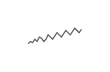
\begin{tikzpicture}[x=0.08em, y=0.08em, line width=0.4pt]
                \draw[FooterGray] (0,3) -- (1,4) -- (2,3.5) -- (3,5) -- (4,4) -- (5,6) -- (6,5.5) -- (7,4) -- (8,5) -- (9,7) -- (10,6) -- (11,5) -- (12,6.5) -- (13,8) -- (14,7) -- (15,6) -- (16,7.5) -- (17,9) -- (18,8) -- (19,7) -- (20,8.5) -- (21,10) -- (22,9) -- (23,8) -- (24,9.5);
            \end{tikzpicture}%
        }%
        \hskip0.5cm%
    }%
    \vskip6pt%
}

%=============================================================================
% PACKAGES
%=============================================================================
\usepackage[utf8]{inputenc}
\DeclareUnicodeCharacter{03B1}{\ensuremath{\alpha}}
\usepackage[T1]{fontenc}
\usepackage{amsmath, amssymb, amsthm}
\usepackage{mathtools}
\usepackage{bm}
\usepackage{tikz}
\usetikzlibrary{arrows.meta, positioning, shapes, calc, decorations.pathreplacing, shadings}
\usepackage{booktabs}
\usepackage{multirow}
\usepackage{array}
\usepackage{graphicx}
\usepackage{animate}
\usepackage{hyperref}
\usepackage{colortbl}
\usepackage{listings}
\lstset{language=Python, basicstyle=\ttfamily\scriptsize, keywordstyle=\color{MainBlue}\bfseries,
  commentstyle=\color{Forest}, stringstyle=\color{Crimson}, breaklines=true,
  frame=none, backgroundcolor=\color{VeryLightGray}, xleftmargin=2mm}
\hypersetup{colorlinks=true, linkcolor=MainBlue, urlcolor=MainBlue}
\graphicspath{{../../logos/}{../../charts/}{../../photos/}}
\usepackage{xcolor}
\hfuzz=2pt  % Suppress tiny overfull warnings (<2pt)
\vfuzz=2pt  % Suppress tiny vertical overfull warnings (<2pt)
% \mathrm in the sans-serif family of the slides (beamer resets \mathrm to the serif family at \begin{document};
% this hook runs after beamer's, so WN, Var, RMSE, ... in formulas match the surrounding text)
% Bold vectors and matrices in the same sans-serif family: \mathbf{A} in sans bold (beamer's own \mathbf came out in
% medium weight), and the bold upright Greek capitals of \boldsymbol / \bm (\bSigma, \bPhi, \boldsymbol{\Theta}) in
% cmss bold: bm.sty fixes its "boldoperators" font when it is loaded (serif cmbx), before beamer switches the
% operators to cmss, so it is reset here.
\AtBeginDocument{%
  \SetMathAlphabet{\mathrm}{normal}{\encodingdefault}{\sfdefault}{\mddefault}{n}%
  \SetMathAlphabet{\mathrm}{bold}{\encodingdefault}{\sfdefault}{bx}{n}%
  \SetMathAlphabet{\mathbf}{normal}{\encodingdefault}{\sfdefault}{bx}{n}%
  \SetMathAlphabet{\mathbf}{bold}{\encodingdefault}{\sfdefault}{bx}{n}%
  \SetSymbolFont{boldoperators}{normal}{OT1}{cmss}{bx}{n}%
  \SetSymbolFont{boldoperators}{bold}{OT1}{cmss}{bx}{n}}

%=============================================================================
% QUANTLET COMMANDS
%   \quantlet{<displayed name>}{<url>}       (generic, compatible with the older TSA decks)
%   \tsaquantlet{Ch_05}{TSA_ch5_garch}       -> https://github.com/danpele/Time-Series-Analysis/tree/main/Quantlets/Ch_05/TSA_ch5_garch
%   \qlurl{<folder>} is defined per chapter by the generator (Quantlets/Ch_NN/<folder>)
%=============================================================================
\newcommand{\tsarepo}{https://github.com/danpele/Time-Series-Analysis}
\newcommand{\tsaqlbase}{https://github.com/danpele/Time-Series-Analysis/tree/main/Quantlets}
\newcommand{\quantlet}[2]{%
    \hfill\href{#2}{%
        \raisebox{-0.15em}{
\includegraphics[height=0.7em]{ql_logo.png}}%
        \textcolor{MainBlue}{\tiny\ #1}%
    }%
}
\newcommand{\tsaquantlet}[2]{\quantlet{\detokenize{#2}}{\tsaqlbase/#1/#2}}

%=============================================================================
% NOTEBOOKS (Google Colab)
%   \colaburl{notebooks/EN/chapter5_seminar_notebook.ipynb} -> the Colab link of a file in the TSA repo
%   \nb: the chapter notebook (each seminar deck redefines it with \renewcommand)
%=============================================================================
\newcommand{\colaburl}[1]{https://colab.research.google.com/github/danpele/Time-Series-Analysis/blob/main/#1}
\newcommand{\nb}{https://colab.research.google.com/github/danpele/Time-Series-Analysis/tree/main/notebooks/EN}
\newcommand{\nbname}{notebooks/EN}

%=============================================================================
% SLIDE HELPERS (used by the generators; the same as in MFM)
%=============================================================================
% local font size for list bodies (the preamble forces \normalsize)
\newcommand{\itemsize}[1]{\setbeamertemplate{itemize/enumerate body begin}{#1}\setbeamertemplate{itemize/enumerate subbody begin}{#1}}
\newcommand{\intitle}[1]{{\hypersetup{urlcolor=white}#1}}   % white links inside coloured title bars
\newcommand{\imgcap}[1]{{\scriptsize #1}\\[0.5mm]}          % caption under a photo
\newcommand{\imgcredit}[2]{{\tiny\color{FooterGray}\href{#1}{#2}}}   % image credit: source URL, author/licence
\newcommand{\aiprompt}[1]{{\ttfamily\color{MainBlue}#1}}     % a prompt to an AI assistant

%=============================================================================
% SEMINARS: student version by default; the instructor wrapper *_solutions.tex sets \solutionstrue
%=============================================================================
\makeatletter\@ifundefined{ifsolutions}{\expandafter\newif\csname ifsolutions\endcsname}{}\makeatother
\newcommand{\solonly}[1]{\ifsolutions #1\fi}
\newcommand{\propsub}{\ifsolutions\else\framesubtitle{\ifdefined\tsalang Rezolvarea se discută la seminar\else Solution discussed in class\fi}\fi}

%=============================================================================
% APPENDIX AND CHAPTER LINKS (latex/appendix_links.py writes the calls; it also re-declares these
% macros before \begin{document}, so the decks compile with or without this preamble block)
%=============================================================================
\providecommand{\tsaapplink}[3]{\hypertarget{#2}{}\hyperlink{#1}{\beamergotobutton{#3}}}
\providecommand{\tsaappback}[2]{\begin{tikzpicture}[remember picture,overlay]\node[anchor=south east] at ([xshift=-3mm,yshift=7mm]current page.south east){\hyperlink{#1}{\beamerreturnbutton{#2}}};\end{tikzpicture}}
\providecommand{\tsachlink}[2]{\href{#1}{#2}}
\providecommand{\tsachlinkt}[2]{\href{#1}{\usebeamercolor[fg]{frametitle}#2}}

%=============================================================================
% QUANTINAR COMMAND: link către un curs Quantinar (subiecte avansate)
%=============================================================================
\newcommand{\quantinar}[2]{%
    \href{#2}{%
        \raisebox{-0.15em}{
\includegraphics[height=0.8em]{qr_logo.png}}%
        \textcolor{MainBlue}{\scriptsize\ #1}%
    }%
}

%=============================================================================
% CUSTOM TITLE PAGE
%=============================================================================
\defbeamertemplate*{title page}{hybrid}[1][]
{
    \vspace{0.2cm}
    % Logos row - top header (with clickable links)
    \begin{center}
        \href{https://www.ase.ro}{
\includegraphics[height=1.0cm]{ase_logo.png}}\hspace{0.3cm}%
        \href{https://theida.net}{
\includegraphics[height=1.0cm]{ida_logo.png}}\hspace{0.3cm}%
        \href{https://blockchain-research-center.com}{
\includegraphics[height=1.0cm]{brc_logo.png}}\hspace{0.3cm}%
        \href{https://www.ai4efin.ase.ro}{
\includegraphics[height=1.0cm]{ai4efin_logo.png}}\hspace{0.3cm}%
        \href{https://ipe.ro/new}{
\includegraphics[height=1.0cm]{acad_logo.png}}\hspace{0.3cm}%
        \href{https://www.digital-finance-msca.com}{
\includegraphics[height=1.0cm]{msca_logo.png}}%
    \end{center}

    \vspace{0.6cm}

    % Main title with Q logos on sides (with clickable links)
    \begin{center}
        \begin{minipage}{0.1\textwidth}
            \centering
            \href{https://quantlet.com}{
\includegraphics[height=1.1cm]{ql_logo.png}}
        \end{minipage}%
        \begin{minipage}{0.78\textwidth}
            \centering
            {\LARGE\bfseries\usebeamercolor[fg]{title}\inserttitle}

            \vspace{0.3cm}

            {\usebeamerfont{subtitle}\usebeamercolor[fg]{title}\insertsubtitle}
        \end{minipage}%
        \begin{minipage}{0.1\textwidth}
            \centering
            \href{https://quantinar.com}{
\includegraphics[height=1.1cm]{qr_logo.png}}
        \end{minipage}
    \end{center}

    \vspace{0.6cm}

    % Authors (left aligned)
    \hspace{0.5cm}{\usebeamerfont{author}\insertauthor}

    \vspace{0.3cm}

    % Institute/Affiliations (left aligned)
    \hspace{0.5cm}\begin{minipage}[t]{0.9\textwidth}
        \raggedright\small\insertinstitute
    \end{minipage}
}

%=============================================================================
% THEOREM ENVIRONMENTS
%=============================================================================
\theoremstyle{definition}
\setbeamertemplate{theorems}[numbered]
\ifdefined\tsalang
\newtheorem{defn}{Definiție}
\newtheorem{thm}{Teoremă}
\newtheorem{prop}{Propoziție}
\newtheorem{rmk}{Observație}
\else
\newtheorem{defn}{Definition}
\newtheorem{thm}{Theorem}
\newtheorem{prop}{Proposition}
\newtheorem{rmk}{Remark}
\fi

%=============================================================================
% CENTRED MINIPAGE (no extra vertical space)
%=============================================================================
\newenvironment{cminipage}[1]{%
    \par\noindent\hfill\begin{minipage}{#1}\ignorespaces
}{%
    \end{minipage}\hfill\null\par
}

%=============================================================================
% CUSTOM COMMANDS
%=============================================================================
\newcommand{\E}{\mathbb{E}}
\newcommand{\Var}{\text{Var}}
\newcommand{\Cov}{\text{Cov}}
\newcommand{\Corr}{\text{Corr}}
\newcommand{\R}{\mathbb{R}}
\newcommand{\N}{\mathbb{N}}
\newcommand{\Z}{\mathbb{Z}}
\newcommand{\B}{\mathbf{B}}
\newcommand{\imark}{\textcolor{MainBlue}{\textbullet}}
\newcommand{\RMSE}{\text{RMSE}}
\newcommand{\MAE}{\text{MAE}}
\newcommand{\MAPE}{\text{MAPE}}

% Boldface vector/matrix commands (VAR, VECM, state space; also used by the older TSA decks)
\newcommand{\bY}{\mathbf{Y}}
\newcommand{\bX}{\mathbf{X}}
\newcommand{\bA}{\mathbf{A}}
\newcommand{\bB}{\mathbf{B}}
\newcommand{\bepsilon}{\boldsymbol{\varepsilon}}
\newcommand{\bSigma}{\boldsymbol{\Sigma}}
\newcommand{\bPhi}{\boldsymbol{\Phi}}
\newcommand{\bGamma}{\boldsymbol{\Gamma}}
\newcommand{\bPi}{\boldsymbol{\Pi}}
\newcommand{\bc}{\mathbf{c}}
\newcommand{\balpha}{\boldsymbol{\alpha}}
\newcommand{\bbeta}{\boldsymbol{\beta}}
\newcommand{\bvarepsilon}{\boldsymbol{\varepsilon}}

% Legacy seminar marks (older TSA seminar decks)
\newcommand{\correct}{\textcolor{Forest}{\checkmark}}
\newcommand{\incorrect}{\textcolor{Crimson}{\texttimes}}
 se definește
%   \newcommand{\coursename}{Time Series Analysis}      (EN)
%   \newcommand{\coursename}{Serii de timp}       (RO)  și  \def\tsalang{ro}
% Fișierele .tex se află în EN/Courses, EN/Seminars, RO/Cursuri, RO/Seminarii (două niveluri sub rădăcină).
% Deck-urile sînt generate de latex/build_chapterN.py / build_seminarN.py (vezi latex/tsa_build.py).

\documentclass[9pt, aspectratio=169, t]{beamer}
\providecommand{\coursename}{Time Series Analysis}

% Ensure content fits on slides
\setbeamersize{text margin left=8mm, text margin right=8mm}
% Smaller institute font (title page)
\setbeamerfont{institute}{size=\footnotesize}

%=============================================================================
% THEME AND STYLE CONFIGURATION
%=============================================================================
\usetheme{default}
% Using default theme for clean header/footer control

% Color Palette (matching Redispatch PDF)
\definecolor{MainBlue}{RGB}{26, 58, 110}
\definecolor{AccentBlue}{RGB}{26, 58, 110}
\definecolor{IDAred}{RGB}{205, 0, 0}
\definecolor{DarkGray}{RGB}{51, 51, 51}
\definecolor{MediumGray}{RGB}{128, 128, 128}
\definecolor{LightGray}{RGB}{248, 248, 248}
\definecolor{VeryLightGray}{RGB}{235, 235, 235}
\definecolor{KeynoteGray}{RGB}{218, 218, 218}
\definecolor{SectionGray}{RGB}{120, 120, 120}
\definecolor{FooterGray}{RGB}{100, 100, 100}
\definecolor{Crimson}{RGB}{220, 53, 69}
\definecolor{Forest}{RGB}{46, 125, 50}
\definecolor{Amber}{RGB}{181, 133, 63}
\definecolor{Orange}{RGB}{230, 126, 34}
\definecolor{Purple}{RGB}{142, 68, 173}

% Gradient background (exact Keynote 315° gradient: white to RGB 218,218,218)
\setbeamertemplate{background}{%
    \begin{tikzpicture}[remember picture, overlay]
        \shade[shading=axis, shading angle=315,
        top color=white, bottom color=KeynoteGray]
        (current page.south west) rectangle (current page.north east);
    \end{tikzpicture}%
}
% Fallback solid color for compatibility
\setbeamercolor{background canvas}{bg=}

\setbeamercolor{palette primary}{bg=MainBlue, fg=white}
\setbeamercolor{palette secondary}{bg=MainBlue!85, fg=white}
\setbeamercolor{palette tertiary}{bg=MainBlue!70, fg=white}
\setbeamercolor{structure}{fg=MainBlue}
\setbeamercolor{title}{fg=IDAred}
\setbeamercolor{frametitle}{fg=IDAred, bg=}
\setbeamercolor{block title}{bg=MainBlue, fg=white}
\setbeamercolor{block body}{bg=VeryLightGray, fg=DarkGray}
\setbeamercolor{block title alerted}{bg=Crimson, fg=white}
\setbeamercolor{block body alerted}{bg=Crimson!8, fg=DarkGray}
\setbeamercolor{block title example}{bg=Forest, fg=white}
\setbeamercolor{block body example}{bg=Forest!8, fg=DarkGray}
\setbeamercolor{item}{fg=MainBlue}

% Footer colors (override Madrid theme blue)
\setbeamercolor{author in head/foot}{fg=FooterGray, bg=}
\setbeamercolor{title in head/foot}{fg=FooterGray, bg=}
\setbeamercolor{date in head/foot}{fg=FooterGray, bg=}
\setbeamercolor{section in head/foot}{fg=FooterGray, bg=}
\setbeamercolor{subsection in head/foot}{fg=FooterGray, bg=}

% Bullet styles (apply everywhere including blocks)
\setbeamertemplate{itemize item}{\color{MainBlue}$\boxdot$}
\setbeamertemplate{itemize subitem}{\color{MainBlue}$\blacktriangleright$}
\setbeamertemplate{itemize subsubitem}{\color{MainBlue}\tiny$\bullet$}
\setbeamertemplate{itemize/enumerate body begin}{\normalsize}
\setbeamertemplate{itemize/enumerate subbody begin}{\normalsize}

% Item spacing - compact style
\setlength{\leftmargini}{10pt}       % Level 1: minimal indent
\setlength{\leftmarginii}{10pt}      % Level 2: minimal additional indent
% Compact list spacing (zero extra space before/after lists in blocks)
\makeatletter
\def\@listi{\leftmargin\leftmargini \topsep 0pt \parsep 0pt \itemsep 0pt}
\def\@listii{\leftmargin\leftmarginii \topsep 0pt \parsep 0pt \itemsep 0pt}
\makeatother

\setbeamertemplate{navigation symbols}{}

%=============================================================================
% CUSTOM HEADLINE
%=============================================================================
\setbeamertemplate{headline}{%
    \vskip10pt%
    \hbox to \paperwidth{%
        \hskip0.5cm%
        {\small\color{FooterGray}\renewcommand{\hyperlink}[2]{##2}\insertsectionhead}%
        \hfill%
        \textcolor{FooterGray}{\small\insertframenumber}%
        \hskip0.5cm%
    }%
    \vskip4pt%
    {\color{FooterGray}\hrule height 0.4pt}%
}

%=============================================================================
% CUSTOM FOOTER
%=============================================================================
\usepackage{fontawesome5}

\setbeamertemplate{footline}{%
    {\color{FooterGray}\hrule height 0.4pt}%
    \vskip4pt%
    \hbox to \paperwidth{%
        \hskip0.5cm%
        \textcolor{FooterGray}{\small\coursename}%
        \hfill%
        \raisebox{-0.1em}{%
            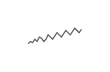
\begin{tikzpicture}[x=0.08em, y=0.08em, line width=0.4pt]
                \draw[FooterGray] (0,3) -- (1,4) -- (2,3.5) -- (3,5) -- (4,4) -- (5,6) -- (6,5.5) -- (7,4) -- (8,5) -- (9,7) -- (10,6) -- (11,5) -- (12,6.5) -- (13,8) -- (14,7) -- (15,6) -- (16,7.5) -- (17,9) -- (18,8) -- (19,7) -- (20,8.5) -- (21,10) -- (22,9) -- (23,8) -- (24,9.5);
            \end{tikzpicture}%
        }%
        \hskip0.5cm%
    }%
    \vskip6pt%
}

%=============================================================================
% PACKAGES
%=============================================================================
\usepackage[utf8]{inputenc}
\DeclareUnicodeCharacter{03B1}{\ensuremath{\alpha}}
\usepackage[T1]{fontenc}
\usepackage{amsmath, amssymb, amsthm}
\usepackage{mathtools}
\usepackage{bm}
\usepackage{tikz}
\usetikzlibrary{arrows.meta, positioning, shapes, calc, decorations.pathreplacing, shadings}
\usepackage{booktabs}
\usepackage{multirow}
\usepackage{array}
\usepackage{graphicx}
\usepackage{animate}
\usepackage{hyperref}
\usepackage{colortbl}
\usepackage{listings}
\lstset{language=Python, basicstyle=\ttfamily\scriptsize, keywordstyle=\color{MainBlue}\bfseries,
  commentstyle=\color{Forest}, stringstyle=\color{Crimson}, breaklines=true,
  frame=none, backgroundcolor=\color{VeryLightGray}, xleftmargin=2mm}
\hypersetup{colorlinks=true, linkcolor=MainBlue, urlcolor=MainBlue}
\graphicspath{{../../logos/}{../../charts/}{../../photos/}}
\usepackage{xcolor}
\hfuzz=2pt  % Suppress tiny overfull warnings (<2pt)
\vfuzz=2pt  % Suppress tiny vertical overfull warnings (<2pt)
% \mathrm in the sans-serif family of the slides (beamer resets \mathrm to the serif family at \begin{document};
% this hook runs after beamer's, so WN, Var, RMSE, ... in formulas match the surrounding text)
% Bold vectors and matrices in the same sans-serif family: \mathbf{A} in sans bold (beamer's own \mathbf came out in
% medium weight), and the bold upright Greek capitals of \boldsymbol / \bm (\bSigma, \bPhi, \boldsymbol{\Theta}) in
% cmss bold: bm.sty fixes its "boldoperators" font when it is loaded (serif cmbx), before beamer switches the
% operators to cmss, so it is reset here.
\AtBeginDocument{%
  \SetMathAlphabet{\mathrm}{normal}{\encodingdefault}{\sfdefault}{\mddefault}{n}%
  \SetMathAlphabet{\mathrm}{bold}{\encodingdefault}{\sfdefault}{bx}{n}%
  \SetMathAlphabet{\mathbf}{normal}{\encodingdefault}{\sfdefault}{bx}{n}%
  \SetMathAlphabet{\mathbf}{bold}{\encodingdefault}{\sfdefault}{bx}{n}%
  \SetSymbolFont{boldoperators}{normal}{OT1}{cmss}{bx}{n}%
  \SetSymbolFont{boldoperators}{bold}{OT1}{cmss}{bx}{n}}

%=============================================================================
% QUANTLET COMMANDS
%   \quantlet{<displayed name>}{<url>}       (generic, compatible with the older TSA decks)
%   \tsaquantlet{Ch_05}{TSA_ch5_garch}       -> https://github.com/danpele/Time-Series-Analysis/tree/main/Quantlets/Ch_05/TSA_ch5_garch
%   \qlurl{<folder>} is defined per chapter by the generator (Quantlets/Ch_NN/<folder>)
%=============================================================================
\newcommand{\tsarepo}{https://github.com/danpele/Time-Series-Analysis}
\newcommand{\tsaqlbase}{https://github.com/danpele/Time-Series-Analysis/tree/main/Quantlets}
\newcommand{\quantlet}[2]{%
    \hfill\href{#2}{%
        \raisebox{-0.15em}{
\includegraphics[height=0.7em]{ql_logo.png}}%
        \textcolor{MainBlue}{\tiny\ #1}%
    }%
}
\newcommand{\tsaquantlet}[2]{\quantlet{\detokenize{#2}}{\tsaqlbase/#1/#2}}

%=============================================================================
% NOTEBOOKS (Google Colab)
%   \colaburl{notebooks/EN/chapter5_seminar_notebook.ipynb} -> the Colab link of a file in the TSA repo
%   \nb: the chapter notebook (each seminar deck redefines it with \renewcommand)
%=============================================================================
\newcommand{\colaburl}[1]{https://colab.research.google.com/github/danpele/Time-Series-Analysis/blob/main/#1}
\newcommand{\nb}{https://colab.research.google.com/github/danpele/Time-Series-Analysis/tree/main/notebooks/EN}
\newcommand{\nbname}{notebooks/EN}

%=============================================================================
% SLIDE HELPERS (used by the generators; the same as in MFM)
%=============================================================================
% local font size for list bodies (the preamble forces \normalsize)
\newcommand{\itemsize}[1]{\setbeamertemplate{itemize/enumerate body begin}{#1}\setbeamertemplate{itemize/enumerate subbody begin}{#1}}
\newcommand{\intitle}[1]{{\hypersetup{urlcolor=white}#1}}   % white links inside coloured title bars
\newcommand{\imgcap}[1]{{\scriptsize #1}\\[0.5mm]}          % caption under a photo
\newcommand{\imgcredit}[2]{{\tiny\color{FooterGray}\href{#1}{#2}}}   % image credit: source URL, author/licence
\newcommand{\aiprompt}[1]{{\ttfamily\color{MainBlue}#1}}     % a prompt to an AI assistant

%=============================================================================
% SEMINARS: student version by default; the instructor wrapper *_solutions.tex sets \solutionstrue
%=============================================================================
\makeatletter\@ifundefined{ifsolutions}{\expandafter\newif\csname ifsolutions\endcsname}{}\makeatother
\newcommand{\solonly}[1]{\ifsolutions #1\fi}
\newcommand{\propsub}{\ifsolutions\else\framesubtitle{\ifdefined\tsalang Rezolvarea se discută la seminar\else Solution discussed in class\fi}\fi}

%=============================================================================
% APPENDIX AND CHAPTER LINKS (latex/appendix_links.py writes the calls; it also re-declares these
% macros before \begin{document}, so the decks compile with or without this preamble block)
%=============================================================================
\providecommand{\tsaapplink}[3]{\hypertarget{#2}{}\hyperlink{#1}{\beamergotobutton{#3}}}
\providecommand{\tsaappback}[2]{\begin{tikzpicture}[remember picture,overlay]\node[anchor=south east] at ([xshift=-3mm,yshift=7mm]current page.south east){\hyperlink{#1}{\beamerreturnbutton{#2}}};\end{tikzpicture}}
\providecommand{\tsachlink}[2]{\href{#1}{#2}}
\providecommand{\tsachlinkt}[2]{\href{#1}{\usebeamercolor[fg]{frametitle}#2}}

%=============================================================================
% QUANTINAR COMMAND: link către un curs Quantinar (subiecte avansate)
%=============================================================================
\newcommand{\quantinar}[2]{%
    \href{#2}{%
        \raisebox{-0.15em}{
\includegraphics[height=0.8em]{qr_logo.png}}%
        \textcolor{MainBlue}{\scriptsize\ #1}%
    }%
}

%=============================================================================
% CUSTOM TITLE PAGE
%=============================================================================
\defbeamertemplate*{title page}{hybrid}[1][]
{
    \vspace{0.2cm}
    % Logos row - top header (with clickable links)
    \begin{center}
        \href{https://www.ase.ro}{
\includegraphics[height=1.0cm]{ase_logo.png}}\hspace{0.3cm}%
        \href{https://theida.net}{
\includegraphics[height=1.0cm]{ida_logo.png}}\hspace{0.3cm}%
        \href{https://blockchain-research-center.com}{
\includegraphics[height=1.0cm]{brc_logo.png}}\hspace{0.3cm}%
        \href{https://www.ai4efin.ase.ro}{
\includegraphics[height=1.0cm]{ai4efin_logo.png}}\hspace{0.3cm}%
        \href{https://ipe.ro/new}{
\includegraphics[height=1.0cm]{acad_logo.png}}\hspace{0.3cm}%
        \href{https://www.digital-finance-msca.com}{
\includegraphics[height=1.0cm]{msca_logo.png}}%
    \end{center}

    \vspace{0.6cm}

    % Main title with Q logos on sides (with clickable links)
    \begin{center}
        \begin{minipage}{0.1\textwidth}
            \centering
            \href{https://quantlet.com}{
\includegraphics[height=1.1cm]{ql_logo.png}}
        \end{minipage}%
        \begin{minipage}{0.78\textwidth}
            \centering
            {\LARGE\bfseries\usebeamercolor[fg]{title}\inserttitle}

            \vspace{0.3cm}

            {\usebeamerfont{subtitle}\usebeamercolor[fg]{title}\insertsubtitle}
        \end{minipage}%
        \begin{minipage}{0.1\textwidth}
            \centering
            \href{https://quantinar.com}{
\includegraphics[height=1.1cm]{qr_logo.png}}
        \end{minipage}
    \end{center}

    \vspace{0.6cm}

    % Authors (left aligned)
    \hspace{0.5cm}{\usebeamerfont{author}\insertauthor}

    \vspace{0.3cm}

    % Institute/Affiliations (left aligned)
    \hspace{0.5cm}\begin{minipage}[t]{0.9\textwidth}
        \raggedright\small\insertinstitute
    \end{minipage}
}

%=============================================================================
% THEOREM ENVIRONMENTS
%=============================================================================
\theoremstyle{definition}
\setbeamertemplate{theorems}[numbered]
\ifdefined\tsalang
\newtheorem{defn}{Definiție}
\newtheorem{thm}{Teoremă}
\newtheorem{prop}{Propoziție}
\newtheorem{rmk}{Observație}
\else
\newtheorem{defn}{Definition}
\newtheorem{thm}{Theorem}
\newtheorem{prop}{Proposition}
\newtheorem{rmk}{Remark}
\fi

%=============================================================================
% CENTRED MINIPAGE (no extra vertical space)
%=============================================================================
\newenvironment{cminipage}[1]{%
    \par\noindent\hfill\begin{minipage}{#1}\ignorespaces
}{%
    \end{minipage}\hfill\null\par
}

%=============================================================================
% CUSTOM COMMANDS
%=============================================================================
\newcommand{\E}{\mathbb{E}}
\newcommand{\Var}{\text{Var}}
\newcommand{\Cov}{\text{Cov}}
\newcommand{\Corr}{\text{Corr}}
\newcommand{\R}{\mathbb{R}}
\newcommand{\N}{\mathbb{N}}
\newcommand{\Z}{\mathbb{Z}}
\newcommand{\B}{\mathbf{B}}
\newcommand{\imark}{\textcolor{MainBlue}{\textbullet}}
\newcommand{\RMSE}{\text{RMSE}}
\newcommand{\MAE}{\text{MAE}}
\newcommand{\MAPE}{\text{MAPE}}

% Boldface vector/matrix commands (VAR, VECM, state space; also used by the older TSA decks)
\newcommand{\bY}{\mathbf{Y}}
\newcommand{\bX}{\mathbf{X}}
\newcommand{\bA}{\mathbf{A}}
\newcommand{\bB}{\mathbf{B}}
\newcommand{\bepsilon}{\boldsymbol{\varepsilon}}
\newcommand{\bSigma}{\boldsymbol{\Sigma}}
\newcommand{\bPhi}{\boldsymbol{\Phi}}
\newcommand{\bGamma}{\boldsymbol{\Gamma}}
\newcommand{\bPi}{\boldsymbol{\Pi}}
\newcommand{\bc}{\mathbf{c}}
\newcommand{\balpha}{\boldsymbol{\alpha}}
\newcommand{\bbeta}{\boldsymbol{\beta}}
\newcommand{\bvarepsilon}{\boldsymbol{\varepsilon}}

% Legacy seminar marks (older TSA seminar decks)
\newcommand{\correct}{\textcolor{Forest}{\checkmark}}
\newcommand{\incorrect}{\textcolor{Crimson}{\texttimes}}
 se definește
%   \newcommand{\coursename}{Time Series Analysis}      (EN)
%   \newcommand{\coursename}{Serii de timp}       (RO)  și  \def\tsalang{ro}
% Fișierele .tex se află în EN/Courses, EN/Seminars, RO/Cursuri, RO/Seminarii (două niveluri sub rădăcină).
% Deck-urile sînt generate de latex/build_chapterN.py / build_seminarN.py (vezi latex/tsa_build.py).

\documentclass[9pt, aspectratio=169, t]{beamer}
\providecommand{\coursename}{Time Series Analysis}

% Ensure content fits on slides
\setbeamersize{text margin left=8mm, text margin right=8mm}
% Smaller institute font (title page)
\setbeamerfont{institute}{size=\footnotesize}

%=============================================================================
% THEME AND STYLE CONFIGURATION
%=============================================================================
\usetheme{default}
% Using default theme for clean header/footer control

% Color Palette (matching Redispatch PDF)
\definecolor{MainBlue}{RGB}{26, 58, 110}
\definecolor{AccentBlue}{RGB}{26, 58, 110}
\definecolor{IDAred}{RGB}{205, 0, 0}
\definecolor{DarkGray}{RGB}{51, 51, 51}
\definecolor{MediumGray}{RGB}{128, 128, 128}
\definecolor{LightGray}{RGB}{248, 248, 248}
\definecolor{VeryLightGray}{RGB}{235, 235, 235}
\definecolor{KeynoteGray}{RGB}{218, 218, 218}
\definecolor{SectionGray}{RGB}{120, 120, 120}
\definecolor{FooterGray}{RGB}{100, 100, 100}
\definecolor{Crimson}{RGB}{220, 53, 69}
\definecolor{Forest}{RGB}{46, 125, 50}
\definecolor{Amber}{RGB}{181, 133, 63}
\definecolor{Orange}{RGB}{230, 126, 34}
\definecolor{Purple}{RGB}{142, 68, 173}

% Gradient background (exact Keynote 315° gradient: white to RGB 218,218,218)
\setbeamertemplate{background}{%
    \begin{tikzpicture}[remember picture, overlay]
        \shade[shading=axis, shading angle=315,
        top color=white, bottom color=KeynoteGray]
        (current page.south west) rectangle (current page.north east);
    \end{tikzpicture}%
}
% Fallback solid color for compatibility
\setbeamercolor{background canvas}{bg=}

\setbeamercolor{palette primary}{bg=MainBlue, fg=white}
\setbeamercolor{palette secondary}{bg=MainBlue!85, fg=white}
\setbeamercolor{palette tertiary}{bg=MainBlue!70, fg=white}
\setbeamercolor{structure}{fg=MainBlue}
\setbeamercolor{title}{fg=IDAred}
\setbeamercolor{frametitle}{fg=IDAred, bg=}
\setbeamercolor{block title}{bg=MainBlue, fg=white}
\setbeamercolor{block body}{bg=VeryLightGray, fg=DarkGray}
\setbeamercolor{block title alerted}{bg=Crimson, fg=white}
\setbeamercolor{block body alerted}{bg=Crimson!8, fg=DarkGray}
\setbeamercolor{block title example}{bg=Forest, fg=white}
\setbeamercolor{block body example}{bg=Forest!8, fg=DarkGray}
\setbeamercolor{item}{fg=MainBlue}

% Footer colors (override Madrid theme blue)
\setbeamercolor{author in head/foot}{fg=FooterGray, bg=}
\setbeamercolor{title in head/foot}{fg=FooterGray, bg=}
\setbeamercolor{date in head/foot}{fg=FooterGray, bg=}
\setbeamercolor{section in head/foot}{fg=FooterGray, bg=}
\setbeamercolor{subsection in head/foot}{fg=FooterGray, bg=}

% Bullet styles (apply everywhere including blocks)
\setbeamertemplate{itemize item}{\color{MainBlue}$\boxdot$}
\setbeamertemplate{itemize subitem}{\color{MainBlue}$\blacktriangleright$}
\setbeamertemplate{itemize subsubitem}{\color{MainBlue}\tiny$\bullet$}
\setbeamertemplate{itemize/enumerate body begin}{\normalsize}
\setbeamertemplate{itemize/enumerate subbody begin}{\normalsize}

% Item spacing - compact style
\setlength{\leftmargini}{10pt}       % Level 1: minimal indent
\setlength{\leftmarginii}{10pt}      % Level 2: minimal additional indent
% Compact list spacing (zero extra space before/after lists in blocks)
\makeatletter
\def\@listi{\leftmargin\leftmargini \topsep 0pt \parsep 0pt \itemsep 0pt}
\def\@listii{\leftmargin\leftmarginii \topsep 0pt \parsep 0pt \itemsep 0pt}
\makeatother

\setbeamertemplate{navigation symbols}{}

%=============================================================================
% CUSTOM HEADLINE
%=============================================================================
\setbeamertemplate{headline}{%
    \vskip10pt%
    \hbox to \paperwidth{%
        \hskip0.5cm%
        {\small\color{FooterGray}\renewcommand{\hyperlink}[2]{##2}\insertsectionhead}%
        \hfill%
        \textcolor{FooterGray}{\small\insertframenumber}%
        \hskip0.5cm%
    }%
    \vskip4pt%
    {\color{FooterGray}\hrule height 0.4pt}%
}

%=============================================================================
% CUSTOM FOOTER
%=============================================================================
\usepackage{fontawesome5}

\setbeamertemplate{footline}{%
    {\color{FooterGray}\hrule height 0.4pt}%
    \vskip4pt%
    \hbox to \paperwidth{%
        \hskip0.5cm%
        \textcolor{FooterGray}{\small\coursename}%
        \hfill%
        \raisebox{-0.1em}{%
            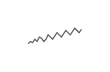
\begin{tikzpicture}[x=0.08em, y=0.08em, line width=0.4pt]
                \draw[FooterGray] (0,3) -- (1,4) -- (2,3.5) -- (3,5) -- (4,4) -- (5,6) -- (6,5.5) -- (7,4) -- (8,5) -- (9,7) -- (10,6) -- (11,5) -- (12,6.5) -- (13,8) -- (14,7) -- (15,6) -- (16,7.5) -- (17,9) -- (18,8) -- (19,7) -- (20,8.5) -- (21,10) -- (22,9) -- (23,8) -- (24,9.5);
            \end{tikzpicture}%
        }%
        \hskip0.5cm%
    }%
    \vskip6pt%
}

%=============================================================================
% PACKAGES
%=============================================================================
\usepackage[utf8]{inputenc}
\DeclareUnicodeCharacter{03B1}{\ensuremath{\alpha}}
\usepackage[T1]{fontenc}
\usepackage{amsmath, amssymb, amsthm}
\usepackage{mathtools}
\usepackage{bm}
\usepackage{tikz}
\usetikzlibrary{arrows.meta, positioning, shapes, calc, decorations.pathreplacing, shadings}
\usepackage{booktabs}
\usepackage{multirow}
\usepackage{array}
\usepackage{graphicx}
\usepackage{animate}
\usepackage{hyperref}
\usepackage{colortbl}
\usepackage{listings}
\lstset{language=Python, basicstyle=\ttfamily\scriptsize, keywordstyle=\color{MainBlue}\bfseries,
  commentstyle=\color{Forest}, stringstyle=\color{Crimson}, breaklines=true,
  frame=none, backgroundcolor=\color{VeryLightGray}, xleftmargin=2mm}
\hypersetup{colorlinks=true, linkcolor=MainBlue, urlcolor=MainBlue}
\graphicspath{{../../logos/}{../../charts/}{../../photos/}}
\usepackage{xcolor}
\hfuzz=2pt  % Suppress tiny overfull warnings (<2pt)
\vfuzz=2pt  % Suppress tiny vertical overfull warnings (<2pt)
% \mathrm in the sans-serif family of the slides (beamer resets \mathrm to the serif family at \begin{document};
% this hook runs after beamer's, so WN, Var, RMSE, ... in formulas match the surrounding text)
% Bold vectors and matrices in the same sans-serif family: \mathbf{A} in sans bold (beamer's own \mathbf came out in
% medium weight), and the bold upright Greek capitals of \boldsymbol / \bm (\bSigma, \bPhi, \boldsymbol{\Theta}) in
% cmss bold: bm.sty fixes its "boldoperators" font when it is loaded (serif cmbx), before beamer switches the
% operators to cmss, so it is reset here.
\AtBeginDocument{%
  \SetMathAlphabet{\mathrm}{normal}{\encodingdefault}{\sfdefault}{\mddefault}{n}%
  \SetMathAlphabet{\mathrm}{bold}{\encodingdefault}{\sfdefault}{bx}{n}%
  \SetMathAlphabet{\mathbf}{normal}{\encodingdefault}{\sfdefault}{bx}{n}%
  \SetMathAlphabet{\mathbf}{bold}{\encodingdefault}{\sfdefault}{bx}{n}%
  \SetSymbolFont{boldoperators}{normal}{OT1}{cmss}{bx}{n}%
  \SetSymbolFont{boldoperators}{bold}{OT1}{cmss}{bx}{n}}

%=============================================================================
% QUANTLET COMMANDS
%   \quantlet{<displayed name>}{<url>}       (generic, compatible with the older TSA decks)
%   \tsaquantlet{Ch_05}{TSA_ch5_garch}       -> https://github.com/danpele/Time-Series-Analysis/tree/main/Quantlets/Ch_05/TSA_ch5_garch
%   \qlurl{<folder>} is defined per chapter by the generator (Quantlets/Ch_NN/<folder>)
%=============================================================================
\newcommand{\tsarepo}{https://github.com/danpele/Time-Series-Analysis}
\newcommand{\tsaqlbase}{https://github.com/danpele/Time-Series-Analysis/tree/main/Quantlets}
\newcommand{\quantlet}[2]{%
    \hfill\href{#2}{%
        \raisebox{-0.15em}{
\includegraphics[height=0.7em]{ql_logo.png}}%
        \textcolor{MainBlue}{\tiny\ #1}%
    }%
}
\newcommand{\tsaquantlet}[2]{\quantlet{\detokenize{#2}}{\tsaqlbase/#1/#2}}

%=============================================================================
% NOTEBOOKS (Google Colab)
%   \colaburl{notebooks/EN/chapter5_seminar_notebook.ipynb} -> the Colab link of a file in the TSA repo
%   \nb: the chapter notebook (each seminar deck redefines it with \renewcommand)
%=============================================================================
\newcommand{\colaburl}[1]{https://colab.research.google.com/github/danpele/Time-Series-Analysis/blob/main/#1}
\newcommand{\nb}{https://colab.research.google.com/github/danpele/Time-Series-Analysis/tree/main/notebooks/EN}
\newcommand{\nbname}{notebooks/EN}

%=============================================================================
% SLIDE HELPERS (used by the generators; the same as in MFM)
%=============================================================================
% local font size for list bodies (the preamble forces \normalsize)
\newcommand{\itemsize}[1]{\setbeamertemplate{itemize/enumerate body begin}{#1}\setbeamertemplate{itemize/enumerate subbody begin}{#1}}
\newcommand{\intitle}[1]{{\hypersetup{urlcolor=white}#1}}   % white links inside coloured title bars
\newcommand{\imgcap}[1]{{\scriptsize #1}\\[0.5mm]}          % caption under a photo
\newcommand{\imgcredit}[2]{{\tiny\color{FooterGray}\href{#1}{#2}}}   % image credit: source URL, author/licence
\newcommand{\aiprompt}[1]{{\ttfamily\color{MainBlue}#1}}     % a prompt to an AI assistant

%=============================================================================
% SEMINARS: student version by default; the instructor wrapper *_solutions.tex sets \solutionstrue
%=============================================================================
\makeatletter\@ifundefined{ifsolutions}{\expandafter\newif\csname ifsolutions\endcsname}{}\makeatother
\newcommand{\solonly}[1]{\ifsolutions #1\fi}
\newcommand{\propsub}{\ifsolutions\else\framesubtitle{\ifdefined\tsalang Rezolvarea se discută la seminar\else Solution discussed in class\fi}\fi}

%=============================================================================
% APPENDIX AND CHAPTER LINKS (latex/appendix_links.py writes the calls; it also re-declares these
% macros before \begin{document}, so the decks compile with or without this preamble block)
%=============================================================================
\providecommand{\tsaapplink}[3]{\hypertarget{#2}{}\hyperlink{#1}{\beamergotobutton{#3}}}
\providecommand{\tsaappback}[2]{\begin{tikzpicture}[remember picture,overlay]\node[anchor=south east] at ([xshift=-3mm,yshift=7mm]current page.south east){\hyperlink{#1}{\beamerreturnbutton{#2}}};\end{tikzpicture}}
\providecommand{\tsachlink}[2]{\href{#1}{#2}}
\providecommand{\tsachlinkt}[2]{\href{#1}{\usebeamercolor[fg]{frametitle}#2}}

%=============================================================================
% QUANTINAR COMMAND: link către un curs Quantinar (subiecte avansate)
%=============================================================================
\newcommand{\quantinar}[2]{%
    \href{#2}{%
        \raisebox{-0.15em}{
\includegraphics[height=0.8em]{qr_logo.png}}%
        \textcolor{MainBlue}{\scriptsize\ #1}%
    }%
}

%=============================================================================
% CUSTOM TITLE PAGE
%=============================================================================
\defbeamertemplate*{title page}{hybrid}[1][]
{
    \vspace{0.2cm}
    % Logos row - top header (with clickable links)
    \begin{center}
        \href{https://www.ase.ro}{
\includegraphics[height=1.0cm]{ase_logo.png}}\hspace{0.3cm}%
        \href{https://theida.net}{
\includegraphics[height=1.0cm]{ida_logo.png}}\hspace{0.3cm}%
        \href{https://blockchain-research-center.com}{
\includegraphics[height=1.0cm]{brc_logo.png}}\hspace{0.3cm}%
        \href{https://www.ai4efin.ase.ro}{
\includegraphics[height=1.0cm]{ai4efin_logo.png}}\hspace{0.3cm}%
        \href{https://ipe.ro/new}{
\includegraphics[height=1.0cm]{acad_logo.png}}\hspace{0.3cm}%
        \href{https://www.digital-finance-msca.com}{
\includegraphics[height=1.0cm]{msca_logo.png}}%
    \end{center}

    \vspace{0.6cm}

    % Main title with Q logos on sides (with clickable links)
    \begin{center}
        \begin{minipage}{0.1\textwidth}
            \centering
            \href{https://quantlet.com}{
\includegraphics[height=1.1cm]{ql_logo.png}}
        \end{minipage}%
        \begin{minipage}{0.78\textwidth}
            \centering
            {\LARGE\bfseries\usebeamercolor[fg]{title}\inserttitle}

            \vspace{0.3cm}

            {\usebeamerfont{subtitle}\usebeamercolor[fg]{title}\insertsubtitle}
        \end{minipage}%
        \begin{minipage}{0.1\textwidth}
            \centering
            \href{https://quantinar.com}{
\includegraphics[height=1.1cm]{qr_logo.png}}
        \end{minipage}
    \end{center}

    \vspace{0.6cm}

    % Authors (left aligned)
    \hspace{0.5cm}{\usebeamerfont{author}\insertauthor}

    \vspace{0.3cm}

    % Institute/Affiliations (left aligned)
    \hspace{0.5cm}\begin{minipage}[t]{0.9\textwidth}
        \raggedright\small\insertinstitute
    \end{minipage}
}

%=============================================================================
% THEOREM ENVIRONMENTS
%=============================================================================
\theoremstyle{definition}
\setbeamertemplate{theorems}[numbered]
\ifdefined\tsalang
\newtheorem{defn}{Definiție}
\newtheorem{thm}{Teoremă}
\newtheorem{prop}{Propoziție}
\newtheorem{rmk}{Observație}
\else
\newtheorem{defn}{Definition}
\newtheorem{thm}{Theorem}
\newtheorem{prop}{Proposition}
\newtheorem{rmk}{Remark}
\fi

%=============================================================================
% CENTRED MINIPAGE (no extra vertical space)
%=============================================================================
\newenvironment{cminipage}[1]{%
    \par\noindent\hfill\begin{minipage}{#1}\ignorespaces
}{%
    \end{minipage}\hfill\null\par
}

%=============================================================================
% CUSTOM COMMANDS
%=============================================================================
\newcommand{\E}{\mathbb{E}}
\newcommand{\Var}{\text{Var}}
\newcommand{\Cov}{\text{Cov}}
\newcommand{\Corr}{\text{Corr}}
\newcommand{\R}{\mathbb{R}}
\newcommand{\N}{\mathbb{N}}
\newcommand{\Z}{\mathbb{Z}}
\newcommand{\B}{\mathbf{B}}
\newcommand{\imark}{\textcolor{MainBlue}{\textbullet}}
\newcommand{\RMSE}{\text{RMSE}}
\newcommand{\MAE}{\text{MAE}}
\newcommand{\MAPE}{\text{MAPE}}

% Boldface vector/matrix commands (VAR, VECM, state space; also used by the older TSA decks)
\newcommand{\bY}{\mathbf{Y}}
\newcommand{\bX}{\mathbf{X}}
\newcommand{\bA}{\mathbf{A}}
\newcommand{\bB}{\mathbf{B}}
\newcommand{\bepsilon}{\boldsymbol{\varepsilon}}
\newcommand{\bSigma}{\boldsymbol{\Sigma}}
\newcommand{\bPhi}{\boldsymbol{\Phi}}
\newcommand{\bGamma}{\boldsymbol{\Gamma}}
\newcommand{\bPi}{\boldsymbol{\Pi}}
\newcommand{\bc}{\mathbf{c}}
\newcommand{\balpha}{\boldsymbol{\alpha}}
\newcommand{\bbeta}{\boldsymbol{\beta}}
\newcommand{\bvarepsilon}{\boldsymbol{\varepsilon}}

% Legacy seminar marks (older TSA seminar decks)
\newcommand{\correct}{\textcolor{Forest}{\checkmark}}
\newcommand{\incorrect}{\textcolor{Crimson}{\texttimes}}


\newcommand{\qlurl}[1]{https://github.com/danpele/Time-Series-Analysis/tree/main/Quantlets/Ch_05/#1}

% Clickable citations (DOIs verified via Crossref)
\newcommand{\refHP}{\href{https://doi.org/10.1007/978-3-031-13584-2}{Huang și Petukhina (2022)}}
\newcommand{\refFPP}{\href{https://otexts.com/fpp3/}{Hyndman și Athanasopoulos (2021)}}
\newcommand{\refTsay}{\href{https://doi.org/10.1002/9780470644560}{Tsay (2010)}}
\newcommand{\refFHH}{\href{https://doi.org/10.1007/978-3-030-13751-9}{Franke, Härdle și Hafner (2019)}}
\newcommand{\refHamilton}{\href{https://doi.org/10.2307/j.ctv14jx6sm}{Hamilton (1994)}}
\newcommand{\refEngle}{\href{https://doi.org/10.2307/1912773}{Engle (1982)}}
\newcommand{\refEngleN}{\href{https://doi.org/10.1257/0002828041464597}{Engle (2004)}}
\newcommand{\refBoll}{\href{https://doi.org/10.1016/0304-4076(86)90063-1}{Bollerslev (1986)}}
\newcommand{\refBollT}{\href{https://doi.org/10.2307/1925546}{Bollerslev (1987)}}
\newcommand{\refEB}{\href{https://doi.org/10.1080/07474938608800095}{Engle și Bollerslev (1986)}}
\newcommand{\refNelson}{\href{https://doi.org/10.2307/2938260}{Nelson (1991)}}
\newcommand{\refGJR}{\href{https://doi.org/10.1111/j.1540-6261.1993.tb05128.x}{Glosten, Jagannathan și Runkle (1993)}}
\newcommand{\refEN}{\href{https://doi.org/10.1111/j.1540-6261.1993.tb05127.x}{Engle și Ng (1993)}}
\newcommand{\refBW}{\href{https://doi.org/10.1080/07474939208800229}{Bollerslev și Wooldridge (1992)}}
\newcommand{\refHansen}{\href{https://doi.org/10.2307/2527081}{Hansen (1994)}}
\newcommand{\refPatton}{\href{https://doi.org/10.1016/j.jeconom.2010.03.034}{Patton (2011)}}
\newcommand{\refHL}{\href{https://doi.org/10.1002/jae.800}{Hansen și Lunde (2005)}}
\newcommand{\refAB}{\href{https://doi.org/10.2307/2527343}{Andersen și Bollerslev (1998)}}
\newcommand{\refChristie}{\href{https://doi.org/10.1016/0304-405X(82)90018-6}{Christie (1982)}}
\newcommand{\refDM}{\href{https://doi.org/10.1080/07350015.1995.10524599}{Diebold și Mariano (1995)}}
\newcommand{\refLB}{\href{https://doi.org/10.1093/biomet/65.2.297}{Ljung și Box (1978)}}
\newcommand{\refML}{\href{https://doi.org/10.1111/j.1467-9892.1983.tb00373.x}{McLeod și Li (1983)}}
\newcommand{\refMandelbrot}{\href{https://doi.org/10.1086/294632}{Mandelbrot (1963)}}
\newcommand{\refRM}{\href{https://www.msci.com/documents/10199/5915b101-4206-4ba0-aee2-3449d5c7e95a}{J.P. Morgan/Reuters (1996)}}
\newcommand{\refAkaike}{\href{https://doi.org/10.1109/TAC.1974.1100705}{Akaike (1974)}}
\newcommand{\refSchwarz}{\href{https://doi.org/10.1214/aos/1176344136}{Schwarz (1978)}}
\newcommand{\refKupiec}{\href{https://doi.org/10.3905/jod.1995.407942}{Kupiec (1995)}}

\title[Serii de timp]{Serii de timp}
\subtitle{Capitolul 5: Volatilitate condiționată: ARCH și GARCH}
\author[D.T. Pele]{Daniel Traian PELE}
\institute{Academia de Studii Economice din București\\
IDA Institute Digital Assets\\
Blockchain Research Center\\
AI4EFin Artificial Intelligence for Energy Finance\\
Academia Română, Institutul de Prognoză Economică\\
MSCA Digital Finance}
\date{}

%=============================================================================
\providecommand{\tsaapplink}[3]{\hypertarget{#2}{}\hyperlink{#1}{\beamergotobutton{#3}}}  % APPLINKS-MACROS
\providecommand{\tsaappback}[2]{\begin{tikzpicture}[remember picture,overlay]\node[anchor=south east] at ([xshift=-3mm,yshift=7mm]current page.south east){\hyperlink{#1}{\beamerreturnbutton{#2}}};\end{tikzpicture}}  % APPLINKS-MACROS
\providecommand{\tsachlink}[2]{\href{#1}{#2}}  % APPLINKS-MACROS
\providecommand{\tsachlinkt}[2]{\href{#1}{\usebeamercolor[fg]{frametitle}#2}}  % APPLINKS-MACROS
\begin{document}
%=============================================================================

{
\setbeamertemplate{headline}{}
\setbeamertemplate{footline}{}
\begin{frame}[noframenumbering]
    \titlepage
\end{frame}
}
% BEGIN-ACRONYMS (generat de latex/acronyms.py; nu editati manual)
\begin{frame}{Acronime folosite în acest material (1/2)}
\setbeamertemplate{itemize/enumerate body begin}{\tiny}
\begin{columns}[T]
\begin{column}{0.49\textwidth}
\begin{itemize}\setlength{\itemsep}{0pt}
    \item \textbf{ACF}: Autocorrelation Function (funcția de autocorelație)
    \item \textbf{AI}: Artificial Intelligence (inteligență artificială)
    \item \textbf{AIC}: Akaike Information Criterion (criteriul informațional Akaike)
    \item \textbf{AR}: AutoRegressive (model); in event studies: Abnormal Return (model autoregresiv; în studiile de eveniment: randament anormal)
    \item \textbf{AR-GARCH}: AR model for the mean with GARCH errors (model AR pentru medie cu erori GARCH)
    \item \textbf{ARCH}: AutoRegressive Conditional Heteroskedasticity (heteroscedasticitate condiționată autoregresivă)
    \item \textbf{ARCH-LM}: ARCH Lagrange Multiplier (test) — testul multiplicatorului Lagrange pentru efecte ARCH
    \item \textbf{ARMA}: AutoRegressive Moving Average (model) — model autoregresiv cu medie mobilă
    \item \textbf{ARMA-GARCH}: ARMA model for the mean with GARCH errors (model ARMA pentru medie cu erori GARCH)
    \item \textbf{BET}: Bucharest Exchange Trading (index) — indicele de referință al Bursei de Valori București
    \item \textbf{BIC}: Bayesian Information Criterion (criteriul informațional bayesian (Schwarz))
    \item \textbf{BNR}: Banca Națională a României
    \item \textbf{BVB}: Bursa de Valori București
\end{itemize}
\end{column}
\begin{column}{0.49\textwidth}
\begin{itemize}\setlength{\itemsep}{0pt}
    \item \textbf{COVID-19}: COronaVIrus Disease 2019 (boala provocată de coronavirus, 2019)
    \item \textbf{DM}: Diebold–Mariano (test) — testul Diebold–Mariano de comparare a prognozelor
    \item \textbf{EGARCH}: Exponential GARCH (GARCH exponențial)
    \item \textbf{EWMA}: Exponentially Weighted Moving Average (medie mobilă ponderată exponențial)
    \item \textbf{GARCH}: Generalised AutoRegressive Conditional Heteroskedasticity (heteroscedasticitate condiționată autoregresivă generalizată)
    \item \textbf{GARCH-N}: GARCH with Normal innovations (GARCH cu inovații Normale)
    \item \textbf{GJR}: Glosten–Jagannathan–Runkle (GARCH model) — modelul GARCH asimetric Glosten–Jagannathan–Runkle
    \item \textbf{GJR-GARCH}: Glosten–Jagannathan–Runkle GARCH (GARCH asimetric Glosten–Jagannathan–Runkle)
    \item \textbf{HAC}: Heteroskedasticity and Autocorrelation Consistent (standard errors) — erori standard robuste la heteroscedasticitate și autocorelație
    \item \textbf{IGARCH}: Integrated GARCH (GARCH integrat)
    \item \textbf{LM}: Lagrange Multiplier (multiplicatorul Lagrange)
    \item \textbf{LR}: Likelihood Ratio (test) — testul raportului de verosimilitate
    \item \textbf{MA}: Moving Average (medie mobilă)
\end{itemize}
\end{column}
\end{columns}
\end{frame}
\begin{frame}{Acronime folosite în acest material (2/2)}
\setbeamertemplate{itemize/enumerate body begin}{\tiny}
\begin{columns}[T]
\begin{column}{0.49\textwidth}
\begin{itemize}\setlength{\itemsep}{0pt}
    \item \textbf{MLE}: Maximum Likelihood Estimation (estimarea prin metoda verosimilității maxime)
    \item \textbf{NIC}: News Impact Curve (curba de impact a știrilor)
    \item \textbf{OLS}: Ordinary Least Squares (metoda celor mai mici pătrate)
    \item \textbf{PACF}: Partial AutoCorrelation Function (funcția de autocorelație parțială)
    \item \textbf{QLIKE}: Quasi-LIKElihood (loss function) — funcția de pierdere de tip cvasi-verosimilitate
    \item \textbf{QMLE}: Quasi-Maximum Likelihood Estimation (estimarea prin cvasi-verosimilitate maximă)
    \item \textbf{QQ}: Quantile–Quantile (plot) — graficul cuantilă–cuantilă
    \item \textbf{SE}: Standard Error (eroare standard)
    \item \textbf{VAR}: Vector AutoRegression (model vector autoregresiv)
\end{itemize}
\end{column}
\begin{column}{0.49\textwidth}
\end{column}
\end{columns}
\end{frame}
% END-ACRONYMS

\begin{frame}{Întrebarea de azi și traseul}
\itemsize{\small}
\begin{itemize}
    \item \textbf{Întrebarea}: dacă randamentul de mîine nu poate fi anticipat, poate fi anticipat \textbf{riscul} de mîine?
    \begin{itemize}
        \item \tsachlink{https://danpele.github.io/Time-Series-Analysis/RO/Cursuri/capitol1_procese_stochastice_stationaritate.pdf}{Capitolele 1}--\tsachlink{https://danpele.github.io/Time-Series-Analysis/RO/Cursuri/capitol3_radacini_unitare_modele_arima.pdf}{3} au modelat \textbf{media} condiționată a unei serii; acest capitol modelează \textbf{varianța} ei condiționată
    \end{itemize}
    \item \textbf{Traseul} capitolului
    \begin{itemize}
        \item faptele stilizate ale randamentelor; ACF a pătratelor randamentelor și testul ARCH-LM
        \item media și varianța condiționată; ARCH($q$) și GARCH(1,1); persistența, IGARCH și EWMA
        \item estimarea prin verosimilitate maximă cu pachetul \texttt{arch}; inovații Student-t; modele ARMA-GARCH
        \item asimetria (GJR, EGARCH), diagnosticarea, prognoza varianței și evaluarea ei, VaR 1\%
    \end{itemize}
    \item Date: S\&P 500, BET, EUR/RON (cursul de referință BNR) și Bitcoin, zilnic; Seminarul 5 are loc înaintea acestui curs
\end{itemize}
\end{frame}

\begin{frame}{Rezultatele învățării}
\itemsize{\small}
\begin{itemize}
    \item Enumerați faptele stilizate ale randamentelor financiare și testați efectele ARCH cu ACF a pătratelor și testul ARCH-LM
    \item Deosebiți varianța condiționată de cea necondiționată și explicați de ce randamentele pot fi necorelate, dar dependente
    \item Scrieți modelele ARCH($q$), GARCH(1,1) și ARMA-GARCH; calculați persistența, varianța de lungă durată și timpul de înjumătățire
    \item Estimați modele GARCH prin verosimilitate maximă în Python, alegeți distribuția inovațiilor și verificați reziduurile standardizate
    \item Măsurați asimetria cu GJR-GARCH, EGARCH și curba de impact a știrilor
    \item Prognozați varianța pe mai multe orizonturi, evaluați prognozele cu QLIKE și calculați un VaR 1\% pe o zi
\end{itemize}
\end{frame}

\begin{frame}{Bibliografie și instrumente}
\itemsize{\small}
\begin{itemize}
    \item Manual: \refHP, cap.~6 (serii de timp financiare: modele ARCH și GARCH)
    \begin{itemize}
        \item lectură suplimentară: \refTsay, cap.~3; \refFHH, cap.~13
    \end{itemize}
    \item Teorie: \refHamilton, cap.~21 (modele de serii de timp cu heteroscedasticitate)
    \item Quantlet-urile Python ale capitolului: \href{https://github.com/danpele/Time-Series-Analysis/tree/main/Quantlets/Ch_05}{Quantlets/Ch\_05}
    \begin{itemize}
        \item estimarea cu pachetul \texttt{arch} (în Colab se instalează cu \texttt{pip install arch}); testele cu \texttt{statsmodels}
    \end{itemize}
    \item Notebook-ul cursului: \href{\colaburl{notebooks/EN/chapter5_lecture_notebook.ipynb}}{deschideți în Google Colab}
    \item Curs video: \quantinar{Applied Time Series Analysis with Python}{https://quantinar.com/course/137/applied-time-series-analysis-with-python}
\end{itemize}
\end{frame}


%=============================================================================
\section{Faptele stilizate ale randamentelor financiare}
%=============================================================================

\begin{frame}{Patru piețe, același tipar}
\itemsize{\footnotesize}
\begin{center}
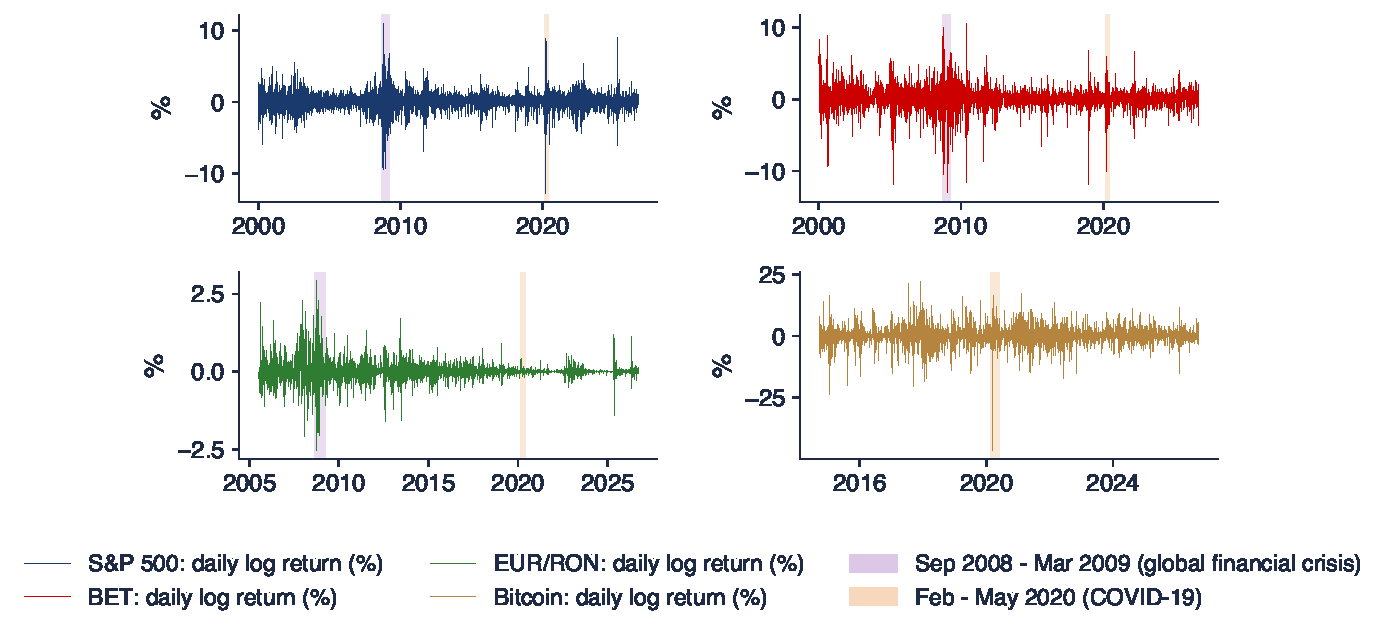
\includegraphics[width=0.97\textwidth,height=0.64\textheight,keepaspectratio]{tsa_ch5_returns.pdf}
\end{center}
\vspace{-0.25cm}
\begin{itemize}
    \item Randamente logaritmice zilnice $r_t = 100(\ln P_t - \ln P_{t-1})$, în \%, pînă la 18 septembrie 2026: S\&P 500 și BET din 2000, EUR/RON (cursul de referință BNR) din iulie 2005, Bitcoin din septembrie 2014
    \item Zonele colorate: criza financiară globală (septembrie 2008 -- martie 2009) și crahul COVID-19 (februarie -- mai 2020)
\end{itemize}
\quantlet{TSA\_ch5\_stylised\_facts}{\qlurl{TSA_ch5_stylised_facts}}
\end{frame}

\begin{frame}{Interpretarea celor patru serii}
\itemsize{\small}
\begin{itemize}
    \item Anii liniștiți alternează cu furtunile: variațiile mari urmează după variații mari, de orice semn
    \begin{itemize}
        \item este fenomenul de \textbf{volatility clustering}, descris prima dată de \refMandelbrot
    \end{itemize}
    \item S\&P 500: abaterea standard zilnică 0{,}42\% în 2017, 3{,}52\% din septembrie 2008 pînă în martie 2009 ($\times$8{,}3) și 3{,}70\% în februarie--mai 2020 ($\times$8{,}8)
    \item EUR/RON: 0{,}78\% în criza din 2008, doar 0{,}10\% în 2020: BNR a menținut leul aproape fix
    \item Un model cu varianță constantă (zgomot alb, \tsachlink{https://danpele.github.io/Time-Series-Analysis/RO/Cursuri/capitol1_procese_stochastice_stationaritate.pdf}{Capitolul 1}) nu descrie niciuna dintre aceste serii
\end{itemize}
\end{frame}

\begin{frame}{Două furtuni: 2008 și 2020}
\itemsize{\footnotesize}
\begin{columns}[T]
\begin{column}{0.48\textwidth}
\centering
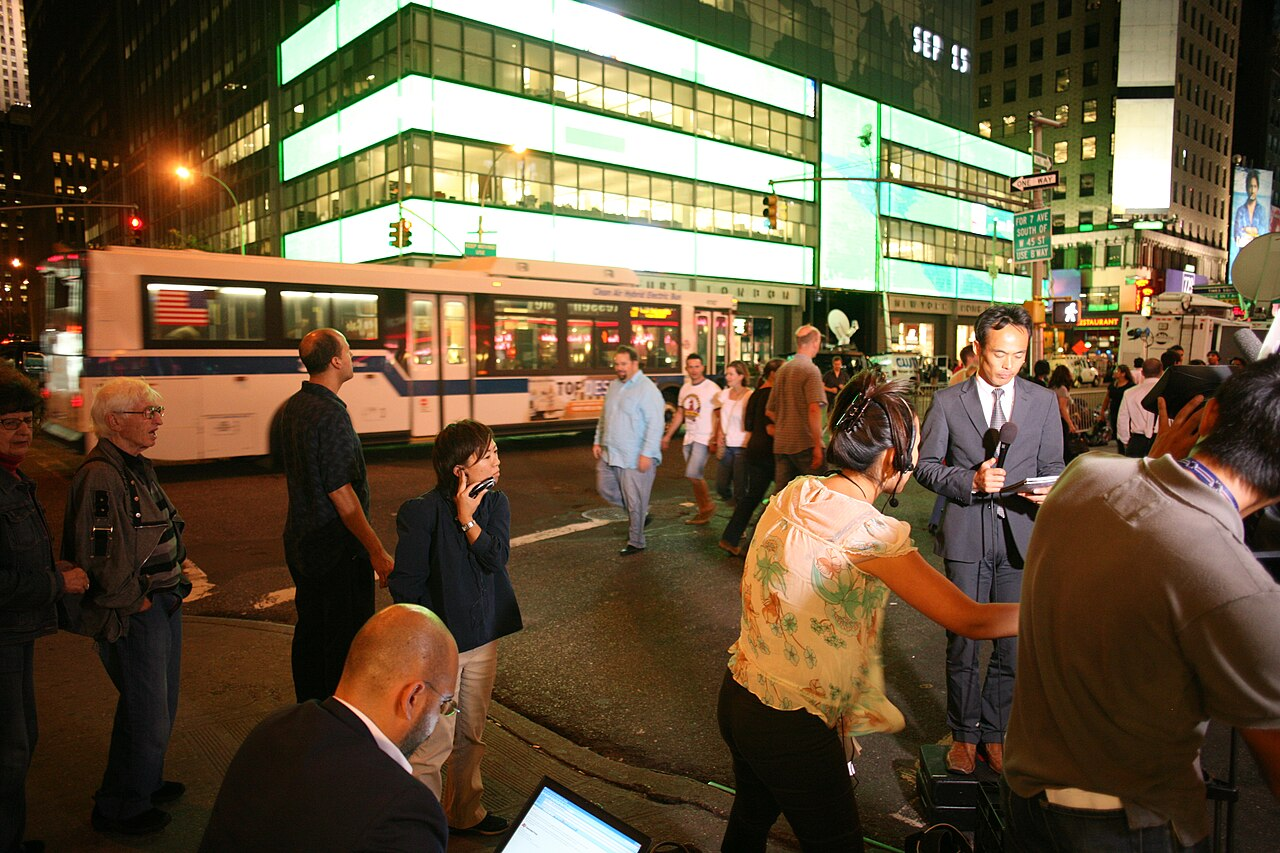
\includegraphics[height=0.42\textheight]{ch5_lehman_2008.jpg}\\[1mm]
\imgcap{Sediul Lehman Brothers, New York, 15 septembrie 2008}
\imgcredit{https://commons.wikimedia.org/wiki/File:Lehman_Brothers-NYC-20080915.jpg}{Foto: Robert Scoble (2008); CC BY 2.0; Wikimedia Commons}
\end{column}
\begin{column}{0.48\textwidth}
\centering

\includegraphics[height=0.42\textheight]{ch5_fidi_2020.jpg}\\[1mm]
\imgcap{Districtul financiar din New York, 25 martie 2020}
\imgcredit{https://commons.wikimedia.org/wiki/File:Subdued_FiDi_(50063555551).jpg}{Foto: Billie Grace Ward (2020); CC BY 2.0; Wikimedia Commons}
\end{column}
\end{columns}\begin{itemize}
    \item 15 septembrie 2008: Lehman Brothers intră în faliment; martie 2020: pandemia COVID-19 închide economiile
    \item În ambele episoade calmul a revenit abia după cîteva luni: un șoc de volatilitate este persistent
\end{itemize}
\end{frame}

\begin{frame}{Faptele stilizate în cifre}
\itemsize{\footnotesize}
\begin{center}
\scriptsize
\begin{tabular}{lrrrrrrrrr}
\toprule
& $T$ & ab. std. & asim. & boltire & $\hat\rho_1(r)$ & $\hat\rho_1(r^2)$ & $Q(10)$, $r$ & $Q(10)$, $r^2$ & LM(5) \\
\midrule
S\&P 500 & 6\,714 & $1{,}21$ & $\ensuremath{-}0{,}35$ & $13{,}7$ & $\ensuremath{-}0{,}10$ & $0{,}31$ & 96 & 6133 & 1684 \\
BET & 6\,670 & $1{,}40$ & $\ensuremath{-}0{,}65$ & $14{,}1$ & $0{,}11$ & $0{,}33$ & 108 & 2440 & 982 \\
EUR/RON & 5\,352 & $0{,}28$ & $0{,}73$ & $18{,}1$ & $0{,}17$ & $0{,}34$ & 222 & 2420 & 871 \\
Bitcoin & 4\,384 & $3{,}49$ & $\ensuremath{-}0{,}70$ & $15{,}0$ & $\ensuremath{-}0{,}02$ & $0{,}14$ & 20 & 213 & 115 \\
\bottomrule
\end{tabular}
\end{center}
\begin{itemize}
    \item \textbf{Cozi groase}: coeficientul de boltire între 13{,}7 și 18{,}1, mult peste 3, valoarea distribuției Normale
    \begin{itemize}
        \item coeficientul de boltire $K = E[(r - \mu)^4]/\sigma^4$; asimetria $E[(r - \mu)^3]/\sigma^3$ (\tsachlink{https://danpele.github.io/Time-Series-Analysis/RO/Cursuri/capitol1_procese_stochastice_stationaritate.pdf}{Capitolul 1})
    \end{itemize}
    \item \textbf{Autocorelație mică în $r_t$}, autocorelație puternică în $r_t^2$: $Q(10)$ al pătratelor este de 11--64 de ori mai mare
    \item $Q(10)$: statistica lui \refLB\ (\tsachlink{https://danpele.github.io/Time-Series-Analysis/RO/Cursuri/capitol1_procese_stochastice_stationaritate.pdf}{Capitolul 1}), $\chi^2(10)$, valoarea de 5\%: 18,31; LM(5): testul ARCH-LM (peste două slide-uri), $\chi^2(5)$, valoarea de 5\%: 11{,}07
\end{itemize}\quantlet{TSA\_ch5\_stylised\_facts}{\qlurl{TSA_ch5_stylised_facts}}
\end{frame}

\begin{frame}{Semnul este imprevizibil, mărimea nu}
\itemsize{\footnotesize}
\begin{center}
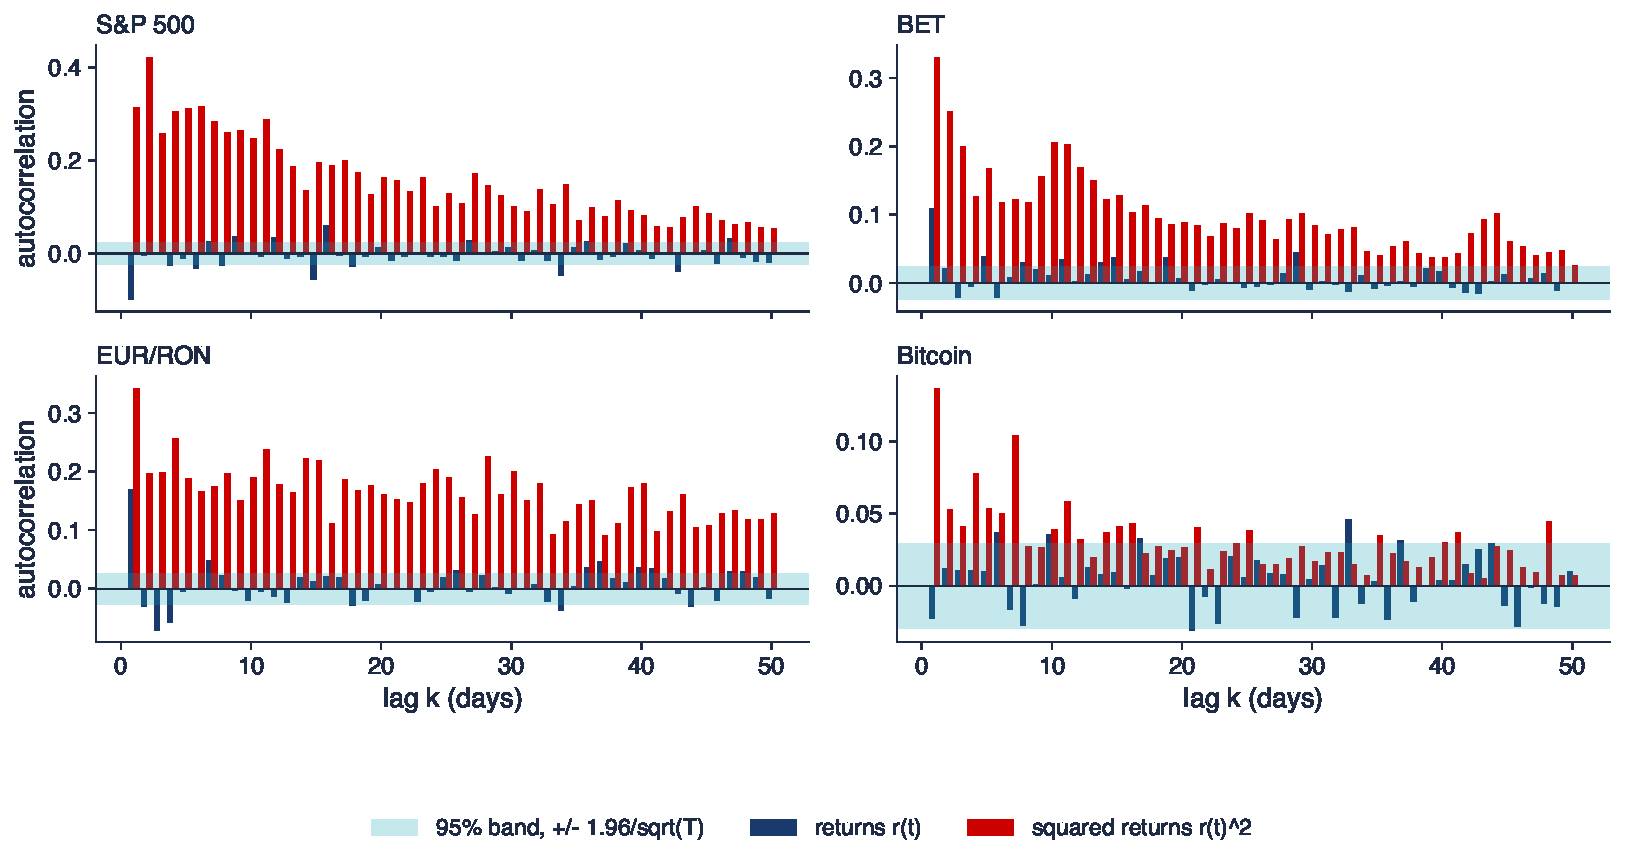
\includegraphics[width=0.97\textwidth,height=0.64\textheight,keepaspectratio]{tsa_ch5_acf_squares.pdf}
\end{center}
\vspace{-0.25cm}
\begin{itemize}
    \item ACF de selecție (autocorrelation function, funcția de autocorelație, \tsachlink{https://danpele.github.io/Time-Series-Analysis/RO/Cursuri/capitol1_procese_stochastice_stationaritate.pdf}{Capitolul 1}) a lui $r_t$ și a lui $r_t^2$, lagurile 1--50, cu banda $\pm 1{,}96/\sqrt{T}$ a unei serii i.i.d.\ (independente și identic distribuite)
\end{itemize}
\quantlet{TSA\_ch5\_stylised\_facts}{\qlurl{TSA_ch5_stylised_facts}}
\end{frame}

\begin{frame}{Interpretarea celor două ACF}
\itemsize{\small}
\begin{itemize}
    \item Randamentele: aproape toate autocorelațiile sînt în bandă (BET: $\hat\rho_1 = 0{,}11$, o piață mai puțin lichidă; \tsachlink{https://danpele.github.io/Time-Series-Analysis/RO/Cursuri/capitol2_modele_arma.pdf}{Capitolul 2})
    \begin{itemize}
        \item direcția variației de mîine este aproape imprevizibilă
    \end{itemize}
    \item Pătratele randamentelor: S\&P 500 0{,}31 la lagul 1 și încă 0{,}05 la lagul 50; 50 din 50 de laguri în afara benzii
    \begin{itemize}
        \item mărimea variației de mîine este previzibilă: o variație mare azi face mai probabilă o variație mare mîine
    \end{itemize}
    \item Necorelat nu înseamnă independent: $r_t$ este apropiat de zgomotul alb, dar nu este i.i.d. (\tsachlink{https://danpele.github.io/Time-Series-Analysis/RO/Cursuri/capitol1_procese_stochastice_stationaritate.pdf}{Capitolul 1})
    \item Bitcoin: mai slab, dar semnificativ ($\hat\rho_1(r_t^2) = 0{,}14$): cîteva zile extreme domină pătratele
\end{itemize}
\end{frame}

\begin{frame}{Testarea efectelor ARCH}
\itemsize{\small}
\begin{itemize}
    \item \textbf{Efecte ARCH}: varianța condiționată depinde de trecut (numele vine de la modelul ARCH, secțiunea 3)
    \item \textbf{Ljung--Box pe pătrate} (testul lui \refML): $Q(m) = T(T+2)\sum_{k=1}^{m}\hat\rho_k^2(\hat\varepsilon^2)/(T-k)$
    \begin{itemize}
        \item $\hat\rho_k(\hat\varepsilon^2)$: autocorelația de selecție a pătratelor reziduurilor la lagul $k$; $m$: numărul de laguri; $T$: numărul de observații
        \item $\hat\varepsilon_t$: reziduurile modelului pentru medie (pentru randamente, $r_t - \bar r$); în ipoteza $H_0$ (fără efecte ARCH), $Q(m) \sim \chi^2(m)$
    \end{itemize}
    \item \textbf{Testul ARCH-LM} \refEngle: test LM (Lagrange multiplier, multiplicatorul Lagrange) din regresia auxiliară
    \begin{itemize}
        \item $\hat\varepsilon_t^2 = b_0 + b_1\hat\varepsilon_{t-1}^2 + \dots + b_q\hat\varepsilon_{t-q}^2 + u_t$, estimată prin OLS (ordinary least squares, metoda celor mai mici pătrate)
        \item $b_0, \dots, b_q$: coeficienții; $q$: numărul de pătrate trecute incluse; $R^2$: coeficientul de determinare al acestei regresii
        \item $H_0$: $b_1 = \dots = b_q = 0$; $\mathrm{LM} = n R^2 \sim \chi^2(q)$, $n$ = numărul de observații din regresie
    \end{itemize}
    \item Ambele teste se aplică reziduurilor modelului pentru medie, înainte și după estimarea unui model de volatilitate
\end{itemize}
\end{frame}

\begin{frame}{Exemplu rezolvat: ARCH-LM pentru BET}
\itemsize{\footnotesize}
\begin{itemize}
    \item Modelul pentru medie: AR(1) pentru randamentele BET (\tsachlink{https://danpele.github.io/Time-Series-Analysis/RO/Cursuri/capitol2_modele_arma.pdf}{Capitolul 2}), $\hat\phi = 0{,}109$; reziduurile $\hat\varepsilon_t$; $q = 5$
    \item Regresia auxiliară (OLS)
    \begin{itemize}
        \item $\hat\varepsilon_t^2 = 0{,}862 + 0{,}276\,\hat\varepsilon_{t-1}^2 + 0{,}099\,\hat\varepsilon_{t-2}^2 + 0{,}088\,\hat\varepsilon_{t-3}^2 + (\ensuremath{-}0{,}015)\,\hat\varepsilon_{t-4}^2 + 0{,}102\,\hat\varepsilon_{t-5}^2$
        \item $R^2 = 0{,}153$, $n = 6\,664$
    \end{itemize}
    \item Pas cu pas: $\mathrm{LM} = n R^2 = 6\,664 \times 0{,}153 = 1017$; valoarea critică de 5\% $\chi^2_{0{,}95}(5) = 11{,}07$
    \begin{itemize}
        \item $1017 \gg 11{,}07$: respingem $H_0$; varianța BET depinde de pătratele ultimelor cinci șocuri
    \end{itemize}
    \item Interpretare: $R^2 = 0{,}153$ este mic, dar pentru pătratele randamentelor este un semnal puternic; următorul pas este un model pentru varianță
\end{itemize}\quantlet{TSA\_ch5\_mean\_model}{\qlurl{TSA_ch5_mean_model}}
\end{frame}

\begin{frame}{Recapitulare: faptele stilizate}
\itemsize{\small}
\begin{itemize}
    \item Cozi groase, volatility clustering, autocorelație mică în $r_t$, autocorelație puternică în $r_t^2$
    \item Efectele ARCH: Ljung--Box pe pătratele reziduurilor, ARCH-LM $= nR^2 \sim \chi^2(q)$
    \item Toate cele patru serii resping $H_0$ la mare distanță de pragul critic
\end{itemize}
\end{frame}


%=============================================================================
\section{Media condiționată și varianța condiționată}
%=============================================================================

\begin{frame}{Condiționarea pe trecut}
\itemsize{\small}
\begin{itemize}
    \item $\mathcal{F}_{t-1}$: informația disponibilă la sfîrșitul zilei $t-1$ (toate valorile trecute)
    \begin{itemize}
        \item speranța condiționată $E[X \mid \mathcal{F}_{t-1}]$: cea mai bună prognoză a lui $X$, dat fiind trecutul (\tsachlink{https://danpele.github.io/Time-Series-Analysis/RO/Cursuri/capitol2_modele_arma.pdf}{Capitolul 2})
    \end{itemize}
    \item \textbf{Media condiționată}: $\mu_t = E[r_t \mid \mathcal{F}_{t-1}]$
    \begin{itemize}
        \item un model ARMA (\tsachlink{https://danpele.github.io/Time-Series-Analysis/RO/Cursuri/capitol2_modele_arma.pdf}{Capitolul 2}) este un model pentru $\mu_t$; pentru randamentele zilnice, $\mu_t$ este mică și aproape constantă
    \end{itemize}
    \item \textbf{Varianța condiționată}: $\sigma_t^2 = \mathrm{Var}(r_t \mid \mathcal{F}_{t-1}) = E[(r_t - \mu_t)^2 \mid \mathcal{F}_{t-1}]$
    \begin{itemize}
        \item $\sigma_t$ este \textbf{volatilitatea condiționată}: cunoscută la $t-1$, se schimbă de la o zi la alta
        \item \textbf{heteroscedasticitate condiționată}: o varianță condiționată care nu este constantă
    \end{itemize}
    \item \textbf{Varianța necondiționată} $\mathrm{Var}(r_t)$: un singur număr pentru tot eșantionul; poate fi constantă în timp ce $\sigma_t^2$ se schimbă
\end{itemize}
\end{frame}

\begin{frame}{Descompunerea de bază}
\itemsize{\small}
\begin{itemize}
    \item Toate modelele din acest capitol: $r_t = \mu_t + \varepsilon_t$, \quad $\varepsilon_t = \sigma_t z_t$
    \begin{itemize}
        \item $z_t$: \textbf{inovațiile}, i.i.d., cu media 0 și varianța 1 (Normale, Student-t, \dots)
        \item $\varepsilon_t$: \textbf{șocul}; $\mu_t$ și $\sigma_t$ depind doar de trecut
    \end{itemize}
    \item Consecințe
    \begin{itemize}
        \item $E[\varepsilon_t \mid \mathcal{F}_{t-1}] = \sigma_t E[z_t] = 0$: șocurile sînt o \textbf{diferență de martingal}, deci sînt necorelate (zgomot alb)
        \item $\mathrm{Var}(\varepsilon_t \mid \mathcal{F}_{t-1}) = \sigma_t^2$: varianța este previzibilă
        \item $\varepsilon_t$ sînt necorelate, dar nu independente: $\varepsilon_t^2$ este corelat cu $\varepsilon_{t-1}^2$
    \end{itemize}
    \item Două modele, cîte unul pentru fiecare moment: ARMA pentru $\mu_t$ (\tsachlink{https://danpele.github.io/Time-Series-Analysis/RO/Cursuri/capitol2_modele_arma.pdf}{Capitolul 2}), GARCH pentru $\sigma_t^2$ (acest capitol); împreună: \textbf{ARMA-GARCH}
\end{itemize}
\end{frame}

\begin{frame}{Exemplu rezolvat: varianța condiționată și varianța necondiționată}
\itemsize{\small}
\begin{itemize}
    \item O piață are zile liniștite ($\sigma_t^2 = 0{,}5$) și zile agitate ($\sigma_t^2 = 4{,}5$), fiecare cu probabilitatea $1/2$; media este 0
    \begin{itemize}
        \item legea varianței totale: $\mathrm{Var}(r_t) = E[\mathrm{Var}(r_t \mid \mathcal{F}_{t-1})] + \mathrm{Var}(E[r_t \mid \mathcal{F}_{t-1}])$
        \item pas cu pas: $0{,}5 \times 0{,}5 + 0{,}5 \times 4{,}5 + 0 = 2{,}50$; abaterea standard necondiționată $1{,}58\%$
    \end{itemize}
    \item Varianța necondiționată este o medie; varianța condiționată ne spune în ce fel de zi ne aflăm
    \begin{itemize}
        \item o zi liniștită: $\sigma_t = 0{,}71\%$; o zi agitată: $\sigma_t = 2{,}12\%$; media de $1{,}58\%$ nu descrie niciuna dintre ele
    \end{itemize}
    \item Cu $z_t$ Normale, amestecul are coeficientul de boltire $3E[\sigma_t^4]/(E[\sigma_t^2])^2 = 4{,}92$: o varianță variabilă în timp creează cozi groase
\end{itemize}
\end{frame}

\begin{frame}{Modelul pentru medie lasă efecte ARCH}
\itemsize{\footnotesize}
\begin{center}
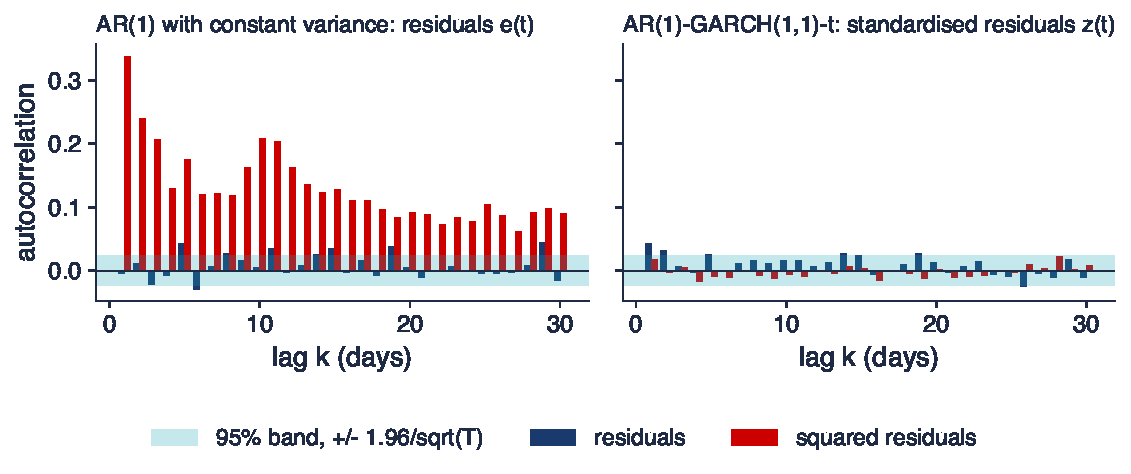
\includegraphics[width=0.97\textwidth,height=0.56\textheight,keepaspectratio]{tsa_ch5_arma_resid.pdf}
\end{center}
\vspace{-0.25cm}
\begin{itemize}
    \item BET: stînga, un AR(1) pentru medie (ordinul ales după BIC dintre AR(0)--AR(5): $p = 1$), cu varianță constantă; dreapta, același AR(1) cu o varianță GARCH(1,1)-t (secțiunea 6)
\end{itemize}
\quantlet{TSA\_ch5\_mean\_model}{\qlurl{TSA_ch5_mean_model}}
\end{frame}

\begin{frame}{Interpretarea ACF ale reziduurilor}
\itemsize{\small}
\begin{itemize}
    \item Stînga: reziduurile arată aproape ca un zgomot alb; verificarea Box--Jenkins din \tsachlink{https://danpele.github.io/Time-Series-Analysis/RO/Cursuri/capitol2_modele_arma.pdf}{Capitolul 2} ar fi aproape trecută
    \begin{itemize}
        \item dar pătratele lor: $\hat\rho_1 = 0{,}34$, $Q(10) = 2496$: efecte ARCH puternice
    \end{itemize}
    \item Dreapta: după împărțirea la $\hat\sigma_t$, pătratele sînt curate: $\hat\rho_1 = 0{,}018$, $Q(10) = 7{,}2$ (p = 0{,}705), ARCH-LM 4{,}8 (p = 0{,}446)
    \begin{itemize}
        \item rămîne puțină autocorelație în nivel ($Q(10) = 28{,}6$): media BET are mai multă structură decît un AR(1)
    \end{itemize}
    \item Lecția: verificăm atît $\hat\varepsilon_t$, cît și $\hat\varepsilon_t^2$; o verificare de zgomot alb doar pe $\hat\varepsilon_t$ nu vede varianța
\end{itemize}
\end{frame}

\begin{frame}{Recapitulare: media și varianța condiționată}
\itemsize{\small}
\begin{itemize}
    \item $r_t = \mu_t + \sigma_t z_t$: $\mu_t$ dintr-un model ARMA, $\sigma_t^2$ dintr-un model de volatilitate
    \item Șocurile sînt necorelate, dar dependente prin pătratele lor
    \item Varianța necondiționată = media varianțelor condiționate; amestecul are cozi groase
\end{itemize}
\end{frame}


%=============================================================================
\section{Modelul ARCH}
%=============================================================================

\begin{frame}{1982: Robert Engle și modelul ARCH}
\itemsize{\footnotesize}
\begin{columns}[T]
\begin{column}{0.60\textwidth}
\begin{itemize}
    \item \refEngle: \textbf{ARCH} (autoregressive conditional heteroskedasticity, heteroscedasticitate condiționată autoregresivă): varianța de azi depinde de pătratele șocurilor de ieri
    \begin{itemize}
        \item prima aplicație: varianța inflației din Regatul Unit, nu o piață financiară
    \end{itemize}
    \item \href{https://www.nobelprize.org/prizes/economic-sciences/2003/summary/}{Premiul Nobel 2003}: „pentru metode de analiză a seriilor de timp economice cu volatilitate variabilă în timp (ARCH)”
    \begin{itemize}
        \item împărțit cu Clive Granger (\tsachlink{https://danpele.github.io/Time-Series-Analysis/RO/Cursuri/capitol3_radacini_unitare_modele_arima.pdf}{Capitolul 3}: regresia falsă; \tsachlink{https://danpele.github.io/Time-Series-Analysis/RO/Cursuri/capitol7_cointegrare_vecm.pdf}{Capitolul 7}: cointegrarea); prelegerea Nobel: \refEngleN
    \end{itemize}
\end{itemize}
\end{column}
\begin{column}{0.36\textwidth}
\centering

\includegraphics[height=0.25\textheight]{ch5_robert_engle_2022.jpg}\\[1mm]
\imgcap{Robert F. Engle (2022)}
\imgcredit{https://commons.wikimedia.org/wiki/File:0603-Kraneshares_KRBN-RobertEngle-JonDemske-16_(cropped).jpg}{Foto: Jon Demske (2022); CC BY-SA 4.0; Wikimedia Commons}\\[1mm]
\centering
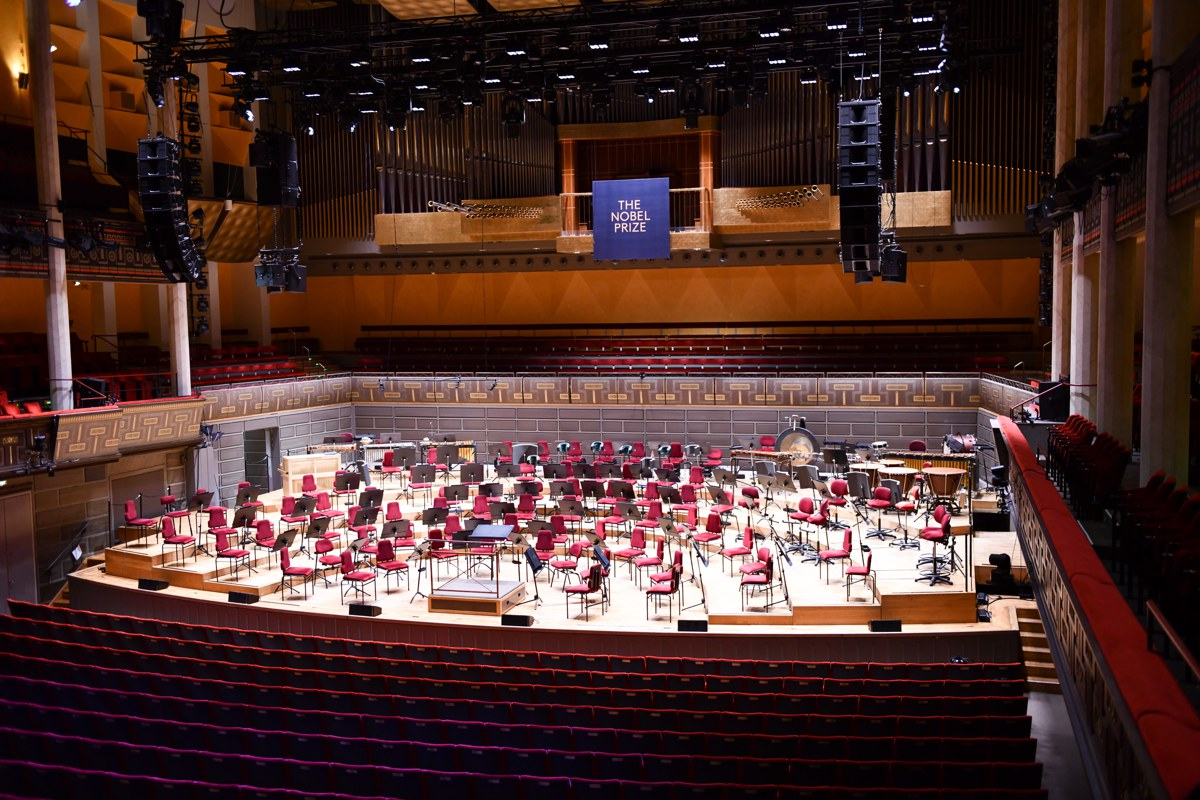
\includegraphics[height=0.16\textheight]{ch5_stockholm_concert_hall.jpg}\\[1mm]
\imgcap{Sala de concerte din Stockholm, unde se decernează Premiile Nobel}
\imgcredit{https://commons.wikimedia.org/wiki/File:Konserthuset_Stockholm_(Stockholm_Concert_Hall).jpg}{Foto: Karen Zhou (2025); CC BY-SA 4.0; Wikimedia Commons}
\end{column}
\end{columns}
\end{frame}

\begin{frame}{ARCH(1): definiție}
\itemsize{\small}
\begin{itemize}
    \item $\varepsilon_t = \sigma_t z_t$, \quad $\sigma_t^2 = \omega + \alpha\,\varepsilon_{t-1}^2$, \quad $\omega > 0$, $\alpha \ge 0$
    \begin{itemize}
        \item $\omega$: nivelul minim al varianței; $\alpha$: cît de puternic reacționează varianța la pătratul șocului de ieri
        \item $\omega > 0$ și $\alpha \ge 0$ asigură o varianță pozitivă
        \item un șoc mare ieri, indiferent de semn, crește varianța de azi
    \end{itemize}
    \item „Autoregresiv”: $\varepsilon_t^2$ urmează un model AR(1) (\tsachlink{https://danpele.github.io/Time-Series-Analysis/RO/Cursuri/capitol2_modele_arma.pdf}{Capitolul 2})
    \begin{itemize}
        \item scriem $\varepsilon_t^2 = \sigma_t^2 + v_t$, cu $v_t = \sigma_t^2(z_t^2 - 1)$ și $E[v_t \mid \mathcal{F}_{t-1}] = 0$
        \item atunci $\varepsilon_t^2 = \omega + \alpha\,\varepsilon_{t-1}^2 + v_t$: un AR(1) pentru pătratele șocurilor, cu erori $v_t$ de tip zgomot alb
    \end{itemize}
    \item De aici, ACF a lui $\varepsilon_t^2$ este $\rho_k = \alpha^k$ (cînd momentul de ordinul patru există): clustering, dar o scădere rapidă
\end{itemize}
\end{frame}

\begin{frame}{ARCH(1): proprietăți}
\itemsize{\small}
\begin{itemize}
    \item $E[\varepsilon_t] = 0$ și $\mathrm{Cov}(\varepsilon_t, \varepsilon_{t-k}) = 0$ pentru $k \ne 0$: zgomot alb
    \item \textbf{Varianța necondiționată} (staționar dacă $\alpha < 1$): aplicăm media în $\sigma_t^2 = \omega + \alpha\varepsilon_{t-1}^2$
    \begin{itemize}
        \item $\bar\sigma^2 = E[\varepsilon_t^2] = \omega + \alpha\bar\sigma^2$, deci $\bar\sigma^2 = \omega/(1 - \alpha)$
    \end{itemize}
    \item \textbf{Coeficientul de boltire} cu $z_t$ Normale (dacă $3\alpha^2 < 1$): $K = 3\,\dfrac{1 - \alpha^2}{1 - 3\alpha^2} > 3$
    \begin{itemize}
        \item inovații Normale, dar șocuri cu cozi groase; dacă $\alpha \ge 1/\sqrt{3} = 0{,}577$, momentul de ordinul patru este infinit
    \end{itemize}
    \item \textbf{Exemplu rezolvat}: $\omega = 0{,}5$, $\alpha = 0{,}5$
    \begin{itemize}
        \item $\bar\sigma^2 = 0{,}5/0{,}5 = 1{,}00$; $K = 3 \times 0{,}75/0{,}25 = 9{,}0$
        \item după un șoc $\varepsilon_{t-1} = 2$: $\sigma_t^2 = 0{,}5 + 0{,}5 \times 4 = 2{,}50$, $\sigma_t = 1{,}58$: varianța se dublează și mai mult
    \end{itemize}
\end{itemize}
\end{frame}

\begin{frame}{Traiectorii simulate: i.i.d., ARCH(1) și GARCH(1,1)}
\itemsize{\footnotesize}
\begin{center}
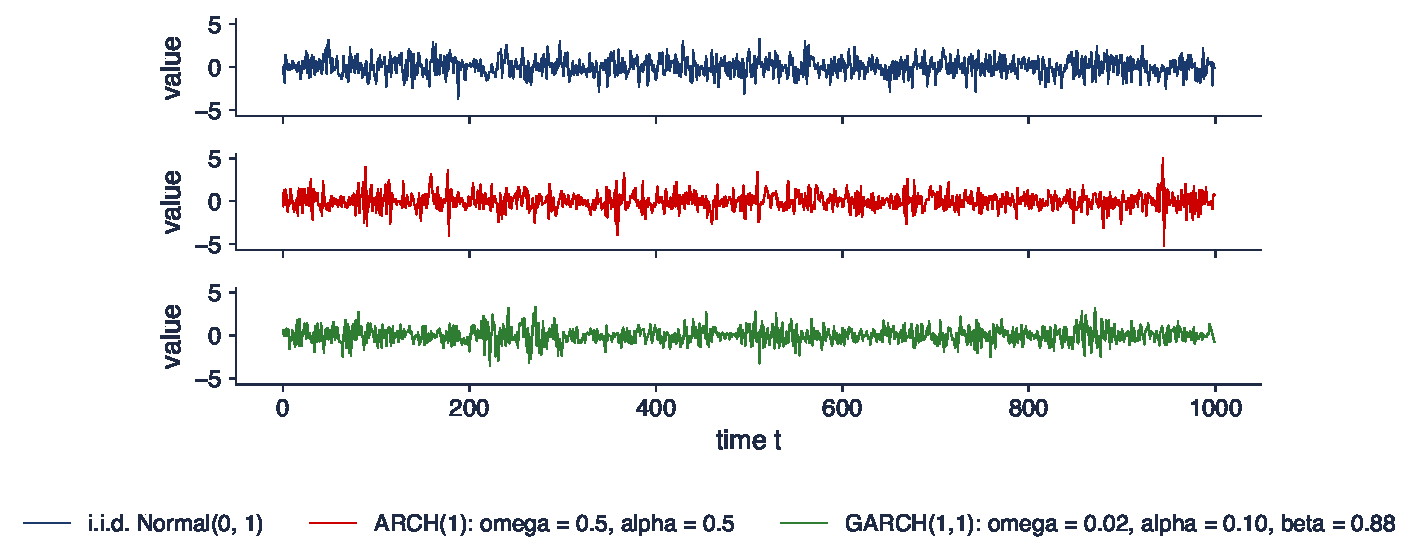
\includegraphics[width=0.97\textwidth,height=0.54\textheight,keepaspectratio]{tsa_ch5_simulated.pdf}
\end{center}
\vspace{-0.25cm}
\begin{itemize}
    \item Trei serii de 1000 de valori cu varianța necondiționată 1: i.i.d.\ Normale; ARCH(1) cu $\omega = \alpha = 0{,}5$; GARCH(1,1) cu $\omega = 0{,}02$, $\alpha = 0{,}10$, $\beta = 0{,}88$ (secțiunea următoare)
    \item Coeficientul de boltire de selecție: i.i.d.\ $3{,}12$, ARCH $4{,}91$, GARCH $3{,}74$ (teoretic: 3, $9{,}0$, $6{,}06$): momentul de ordinul patru converge lent
    \item Interpretare: ARCH(1) produce vîrfuri izolate; GARCH(1,1) produce perioade lungi liniștite și perioade lungi agitate, ca randamentele reale
\end{itemize}
\quantlet{TSA\_ch5\_simulation\_likelihood}{\qlurl{TSA_ch5_simulation_likelihood}}
\end{frame}

\begin{frame}{ARCH($q$) și limitele lui}
\itemsize{\footnotesize}
\begin{itemize}
    \item \textbf{ARCH($q$)}: $\sigma_t^2 = \omega + \alpha_1\varepsilon_{t-1}^2 + \dots + \alpha_q\varepsilon_{t-q}^2$, $\alpha_i \ge 0$; staționar dacă $\sum_i \alpha_i < 1$
    \begin{itemize}
        \item un șoc influențează varianța exact $q$ zile; clustering-ul real durează luni
    \end{itemize}
\end{itemize}\begin{center}
\footnotesize
\begin{tabular}{lrrrrr}
\toprule
S\&P 500, $z_t$ Normale & parametri & log-verosimilitate & AIC & BIC & $\sum\alpha_i$ (+$\beta$) \\
\midrule
ARCH(1) & 3 & $\ensuremath{-}10305{,}5$ & 20617{,}0 & 20637{,}5 & $0{,}394$ \\
ARCH(5) & 7 & $\ensuremath{-}9340{,}5$ & 18695{,}1 & 18742{,}7 & $0{,}816$ \\
ARCH(10) & 12 & $\ensuremath{-}9227{,}6$ & 18479{,}3 & 18561{,}0 & $0{,}849$ \\
GARCH(1,1) & 4 & $\ensuremath{-}9218{,}0$ & \textbf{18444{,}0} & \textbf{18471{,}2} & $0{,}980$ \\
\bottomrule
\end{tabular}
\end{center}
\begin{itemize}
    \item AIC (Akaike) și BIC (Bayesian information criterion, criteriul informațional bayesian): $\mathrm{AIC} = -2\ell + 2k$, $\mathrm{BIC} = -2\ell + k\ln T$ (\tsachlink{https://danpele.github.io/Time-Series-Analysis/RO/Cursuri/capitol2_modele_arma.pdf}{Capitolul 2}), $\ell$: log-verosimilitatea maximizată, $k$: numărul de parametri; valoarea mai mică este mai bună
    \item Interpretare: ARCH are nevoie de zece laguri și tot pierde în fața GARCH(1,1), care are patru parametri: motivația pentru GARCH
\end{itemize}\quantlet{TSA\_ch5\_garch\_estimation}{\qlurl{TSA_ch5_garch_estimation}}
\end{frame}

\begin{frame}{Recapitulare: modelul ARCH}
\itemsize{\small}
\begin{itemize}
    \item $\sigma_t^2 = \omega + \sum_i\alpha_i\varepsilon_{t-i}^2$: un model AR pentru pătratele șocurilor
    \item Varianța necondiționată $\omega/(1 - \sum\alpha_i)$; boltire peste 3 chiar cu inovații Normale
    \item Clustering-ul real cere multe laguri: GARCH le înlocuiește cu un singur parametru în plus
\end{itemize}
\end{frame}


%=============================================================================
\section{Modelul GARCH(1,1)}
%=============================================================================

\begin{frame}{1986: Tim Bollerslev și modelul GARCH}
\itemsize{\small}
\begin{columns}[T]
\begin{column}{0.56\textwidth}
\begin{itemize}
    \item \refBoll, doctorand al lui Engle la University of California, San Diego: adaugă în ecuație varianța de ieri
    \begin{itemize}
        \item \textbf{GARCH} (generalised ARCH, ARCH generalizat): cîțiva parametri înlocuiesc un ARCH($q$) lung
    \end{itemize}
    \item Inovații Student-t pentru randamente: \refBollT
    \item Rămîne modelul de referință: \refHL\ au comparat 330 de modele de volatilitate și au găsit că GARCH(1,1) este greu de depășit la cursurile de schimb
\end{itemize}
\end{column}
\begin{column}{0.40\textwidth}
\centering
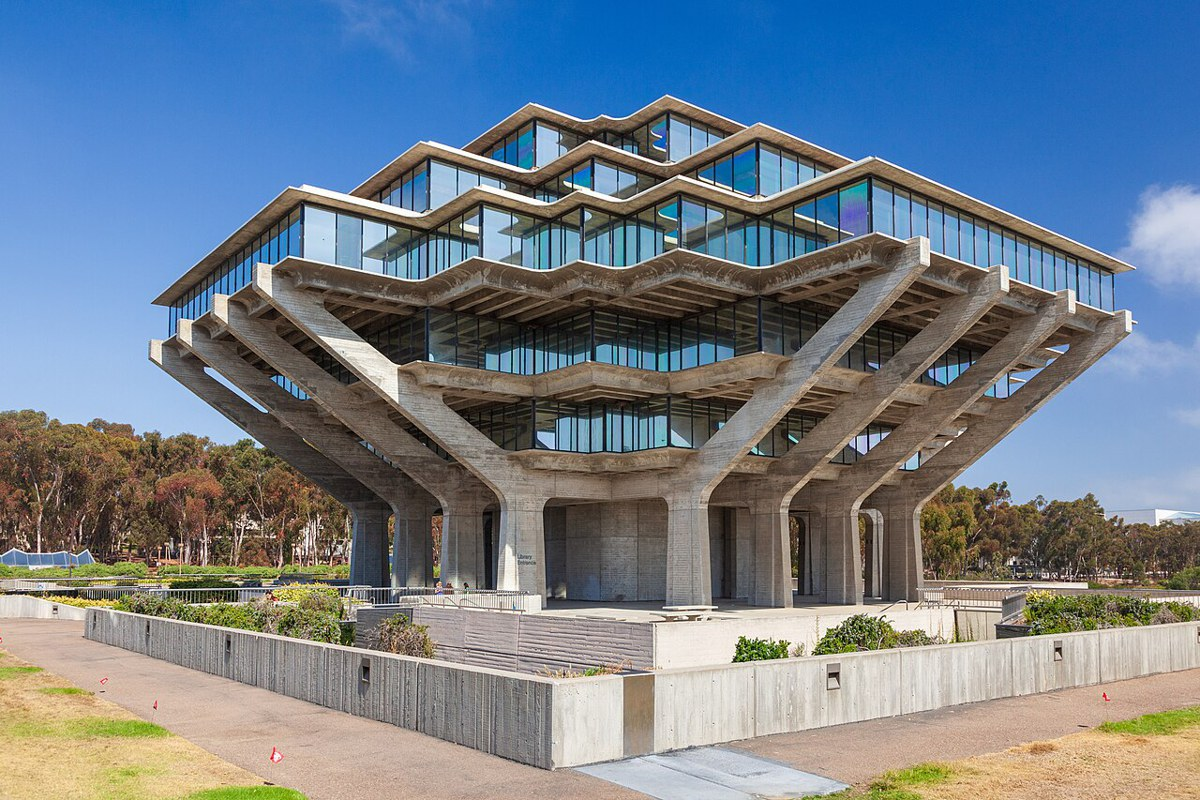
\includegraphics[height=0.36\textheight]{ch5_ucsd_geisel_2010.jpg}\\[1mm]
\imgcap{Biblioteca Geisel, University of California, San Diego}
\imgcredit{https://commons.wikimedia.org/wiki/File:Geisel_Library,_UC_San_Diego.jpg}{Foto: Stephen Bay (2010); CC BY 4.0; Wikimedia Commons}
\end{column}
\end{columns}
\end{frame}

\begin{frame}{GARCH(1,1): definiție}
\itemsize{\small}
\begin{itemize}
    \item $\varepsilon_t = \sigma_t z_t$, \quad $\sigma_t^2 = \omega + \alpha\,\varepsilon_{t-1}^2 + \beta\,\sigma_{t-1}^2$, \quad $\omega > 0$, $\alpha \ge 0$, $\beta \ge 0$
    \begin{itemize}
        \item GARCH($p$,$q$) adaugă mai multe laguri de ambele tipuri; în practică, (1,1) este aproape întotdeauna suficient
    \end{itemize}
    \item Interpretarea parametrilor
    \begin{itemize}
        \item $\alpha$: \textbf{reacția} la știrile de ieri; $\beta$: \textbf{memoria} varianței
        \item $\alpha + \beta$: \textbf{persistența}; $\omega$ fixează nivelul de lungă durată
    \end{itemize}
    \item Prin recurență: un ARCH($\infty$) cu ponderi geometrice
    \begin{itemize}
        \item $\sigma_t^2 = \dfrac{\omega}{1 - \beta} + \alpha\sum_{j=0}^{\infty}\beta^j\,\varepsilon_{t-1-j}^2$: toate șocurile trecute contează, cu ponderi care scad ca $\beta^j$
    \end{itemize}
\end{itemize}
\end{frame}

\begin{frame}{GARCH(1,1) ca ARMA(1,1) pentru pătratele șocurilor}
\itemsize{\small}
\begin{itemize}
    \item Ca la ARCH, scriem $\varepsilon_t^2 = \sigma_t^2 + v_t$ și înlocuim $\sigma_t^2 = \varepsilon_t^2 - v_t$ în ecuație
    \begin{itemize}
        \item $\varepsilon_t^2 = \omega + (\alpha + \beta)\,\varepsilon_{t-1}^2 + v_t - \beta\,v_{t-1}$
        \item un ARMA(1,1) (\tsachlink{https://danpele.github.io/Time-Series-Analysis/RO/Cursuri/capitol2_modele_arma.pdf}{Capitolul 2}) cu coeficientul AR $\alpha + \beta$ și coeficientul MA $-\beta$
    \end{itemize}
    \item Consecințe
    \begin{itemize}
        \item \textbf{staționar în covarianță} dacă $\alpha + \beta < 1$ (rădăcina AR în afara cercului unitate)
        \item ACF a lui $\varepsilon_t^2$ scade ca $(\alpha + \beta)^k$: lent cînd persistența este aproape de 1, ca în ACF a pătratelor randamentelor reale
        \item identificarea prin ACF și PACF (partial autocorrelation function, funcția de autocorelație parțială) a lui $\varepsilon_t^2$ este posibilă în principiu, dar în practică folosim verosimilitatea maximă (secțiunea 5)
    \end{itemize}
\end{itemize}
\end{frame}

\begin{frame}{Varianța de lungă durată, boltirea, persistența și timpul de înjumătățire}
\itemsize{\small}
\begin{itemize}
    \item \textbf{Varianța de lungă durată (necondiționată)}: $\bar\sigma^2 = \omega/(1 - \alpha - \beta)$; volatilitatea anualizată $\sqrt{252\,\bar\sigma^2}$ pentru 252 de zile de tranzacționare
    \begin{itemize}
        \item boltirea cu $z_t$ Normale: $K = 3\,\dfrac{1 - (\alpha + \beta)^2}{1 - (\alpha + \beta)^2 - 2\alpha^2} > 3$; $\alpha = 0{,}10$, $\beta = 0{,}88$: $K = 6{,}06$
    \end{itemize}
    \item O abatere de la $\bar\sigma^2$ se micșorează cu factorul $\alpha + \beta$ în fiecare zi (secțiunea 9): $E_t[\sigma_{t+h}^2] - \bar\sigma^2 = (\alpha + \beta)^{h-1}(\sigma_{t+1}^2 - \bar\sigma^2)$
    \begin{itemize}
        \item $E_t[\cdot]$: media condiționată de informația din ziua $t$; $\sigma_{t+1}^2$: varianța de mîine, cunoscută deja la momentul $t$
        \item \textbf{timpul de înjumătățire}: numărul de zile după care a dispărut jumătate dintr-un șoc de varianță, $h_{1/2} = \ln 0{,}5/\ln(\alpha + \beta)$
        \item $\alpha + \beta = 0{,}90$: 6{,}6 zile; $0{,}98$: 34{,}3 zile; $0{,}99$: 69{,}0 zile: schimbările mici în apropiere de 1 contează mult
    \end{itemize}
\end{itemize}
\end{frame}

\begin{frame}{Exemplu rezolvat: un pas GARCH(1,1)}
\itemsize{\small}
\begin{itemize}
    \item Randamente zilnice în \%: $\omega = 0{,}02$, $\alpha = 0{,}10$, $\beta = 0{,}88$, $\mu = 0$
    \item Mărimile de lungă durată
    \begin{itemize}
        \item persistența $\alpha + \beta = 0{,}98$; $\bar\sigma^2 = 0{,}02/(1 - 0{,}98) = 1{,}00$; volatilitatea anualizată $\sqrt{252 \times 1{,}00} = 15{,}9\%$
        \item timpul de înjumătățire $\ln 0{,}5/\ln 0{,}98 = 34{,}3$ zile
    \end{itemize}
    \item Azi: $\sigma_t^2 = 1{,}2$, iar randamentul este $r_t = -3\%$
    \begin{itemize}
        \item mîine: $\sigma_{t+1}^2 = 0{,}02 + 0{,}10 \times 9 + 0{,}88 \times 1{,}2 = 1{,}976$, $\sigma_{t+1} = 1{,}41\%$
        \item șocul a crescut varianța de la 1,2 la aproape 2; apoi ea scade spre 1{,}00 cu factorul 0{,}98 pe zi
    \end{itemize}
\end{itemize}
\end{frame}

\begin{frame}{IGARCH și legătura cu EWMA}
\itemsize{\small}
\begin{itemize}
    \item \textbf{IGARCH} (integrated GARCH, GARCH integrat) \refEB: $\alpha + \beta = 1$: o rădăcină unitară în ARMA(1,1) pentru $\varepsilon_t^2$ (\tsachlink{https://danpele.github.io/Time-Series-Analysis/RO/Cursuri/capitol3_radacini_unitare_modele_arima.pdf}{Capitolul 3})
    \begin{itemize}
        \item șocurile varianței nu se sting niciodată: nu există timp de înjumătățire și nici varianță necondiționată finită
    \end{itemize}
    \item \textbf{EWMA} (exponentially weighted moving average, media mobilă ponderată exponențial) a \refRM: $\sigma_t^2 = \lambda\sigma_{t-1}^2 + (1 - \lambda)r_{t-1}^2$
    \begin{itemize}
        \item $\lambda \in (0, 1)$: ponderea varianței de ieri; $1 - \lambda$: ponderea pătratului randamentului de ieri
        \item netezirea exponențială simplă (\tsachlink{https://danpele.github.io/Time-Series-Analysis/RO/Cursuri/capitol0_introducere.pdf}{Capitolul 0}) aplicată lui $r_t^2$, cu constanta de netezire $1 - \lambda$
        \item un IGARCH cu $\omega = 0$, $\alpha = 1 - \lambda$, $\beta = \lambda$; RiskMetrics folosește $\lambda = 0{,}94$ pentru date zilnice (timpul de înjumătățire al ponderilor: 11{,}2 zile)
    \end{itemize}
    \item \textbf{Întrebare pentru sală}: imediat după un crah, un analist prognozează volatilitatea peste un an cu EWMA. Unde greșește?
    \begin{itemize}
        \item \textbf{Răspuns}: EWMA păstrează nivelul de criză de azi pentru tot anul; GARCH îl lasă să scadă spre nivelul de lungă durată
    \end{itemize}
\end{itemize}
\end{frame}

\begin{frame}{GARCH, EWMA și o fereastră mobilă în 2020}
\itemsize{\footnotesize}
\begin{center}
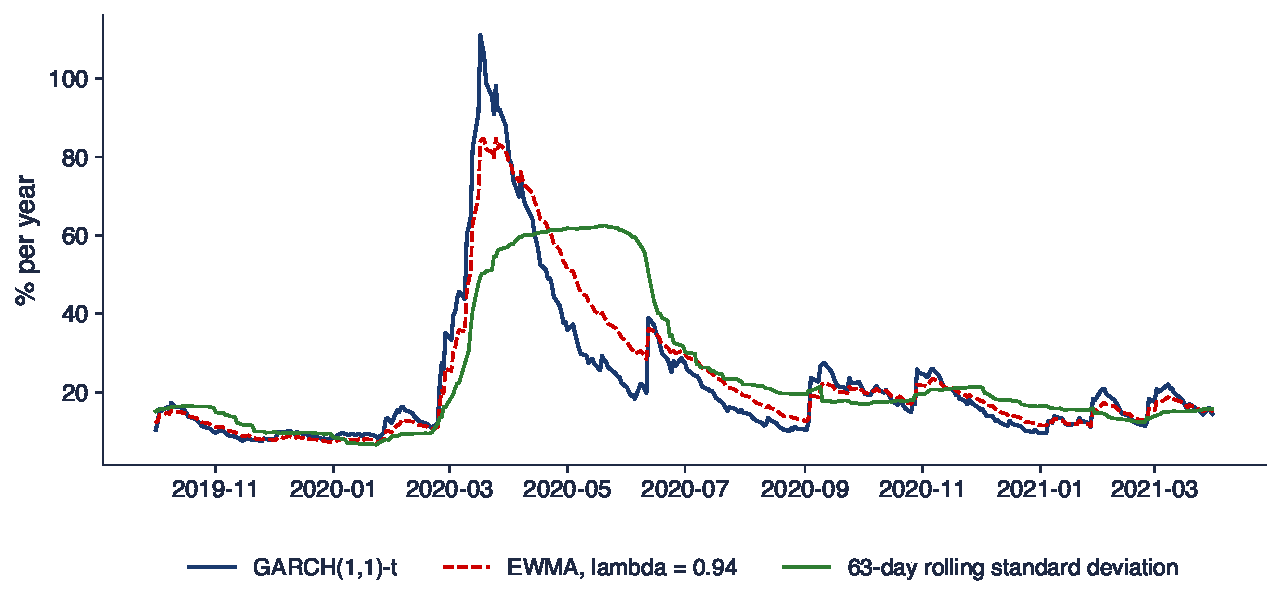
\includegraphics[width=0.97\textwidth,height=0.60\textheight,keepaspectratio]{tsa_ch5_ewma_garch.pdf}
\end{center}
\vspace{-0.25cm}
\begin{itemize}
    \item S\&P 500, volatilitatea anualizată: GARCH(1,1)-t estimat pe toate datele, EWMA cu $\lambda = 0{,}94$ și abaterea standard a ultimelor 63 de zile (\tsachlink{https://danpele.github.io/Time-Series-Analysis/RO/Cursuri/capitol0_introducere.pdf}{Capitolul 0}: o medie mobilă)
\end{itemize}
\quantlet{TSA\_ch5\_volatility\_markets}{\qlurl{TSA_ch5_volatility_markets}}
\end{frame}

\begin{frame}{Interpretarea celor trei estimări}
\itemsize{\small}
\begin{itemize}
    \item Vîrfuri: GARCH 111\% (17 martie 2020), EWMA 85\% (25 martie 2020), fereastra de 63 de zile 63\% (20 mai 2020)
    \item Fereastra mobilă reacționează tîrziu și scade brusc cînd crahul iese din fereastră („fantoma” crahului)
    \begin{itemize}
        \item la 30 iunie 2020: GARCH 28\%, EWMA 30\%, fereastra 32\%
    \end{itemize}
    \item GARCH reacționează cel mai repede ($\alpha$ mai mare decît $1 - \lambda$) și scade cel mai repede (revenire la medie); EWMA este între ele
\end{itemize}
\end{frame}

\begin{frame}{Recapitulare: modelul GARCH(1,1)}
\itemsize{\small}
\begin{itemize}
    \item $\sigma_t^2 = \omega + \alpha\varepsilon_{t-1}^2 + \beta\sigma_{t-1}^2$: reacția $\alpha$, memoria $\beta$; un ARMA(1,1) pentru $\varepsilon_t^2$
    \item $\alpha + \beta < 1$: varianța de lungă durată $\omega/(1 - \alpha - \beta)$, timpul de înjumătățire $\ln 0{,}5/\ln(\alpha + \beta)$
    \item $\alpha + \beta = 1$: IGARCH; EWMA este un IGARCH fără $\omega$
\end{itemize}
\end{frame}


%=============================================================================
\section{Estimarea prin verosimilitate maximă}
%=============================================================================

\begin{frame}{Verosimilitatea unui model GARCH}
\itemsize{\small}
\begin{itemize}
    \item Randamentele sînt dependente, deci densitatea comună este un produs de densități condiționate
    \begin{itemize}
        \item $f(r_1, \dots, r_T) = f(r_1)\prod_{t=2}^{T} f(r_t \mid \mathcal{F}_{t-1})$, cu $r_t \mid \mathcal{F}_{t-1} \sim N(\mu, \sigma_t^2)$ pentru inovații Normale
    \end{itemize}
    \item \textbf{Log-verosimilitatea condiționată}, $\theta = (\mu, \omega, \alpha, \beta)$:
    \begin{itemize}
        \item $\ell(\theta) = -\dfrac12\sum_{t=2}^{T}\Big[\ln(2\pi) + \ln\sigma_t^2(\theta) + \dfrac{(r_t - \mu)^2}{\sigma_t^2(\theta)}\Big]$
        \item $\sigma_t^2(\theta)$ se calculează recursiv, pornind de la o valoare inițială $\sigma_1^2$ (de exemplu, varianța de selecție)
    \end{itemize}
    \item \textbf{MLE} (maximum likelihood estimation, estimarea prin verosimilitate maximă): $\hat\theta = \arg\max_\theta \ell(\theta)$, cu $\omega > 0$, $\alpha, \beta \ge 0$, $\alpha + \beta < 1$
    \begin{itemize}
        \item nu există o formulă explicită: un algoritm numeric caută maximul; OLS nu este posibil, deoarece $\sigma_t^2$ nu este observat
    \end{itemize}
\end{itemize}
\end{frame}

\begin{frame}{Verosimilitatea modelului ARCH(1)}
\itemsize{\footnotesize}
\begin{center}
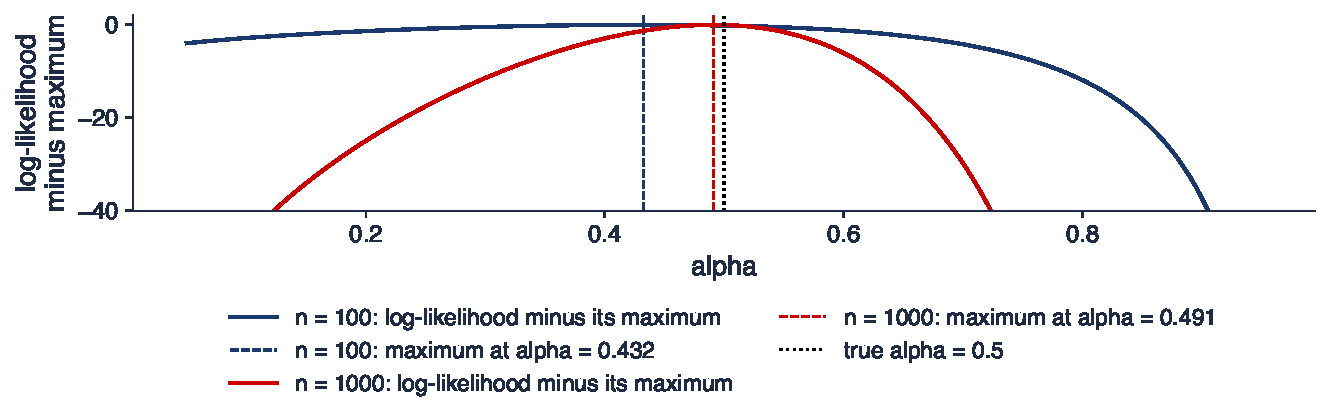
\includegraphics[width=0.97\textwidth,height=0.56\textheight,keepaspectratio]{tsa_ch5_lik_arch1.pdf}
\end{center}
\vspace{-0.25cm}
\begin{itemize}
    \item ARCH(1) simulat cu $\omega = \alpha = 0{,}5$; $\ell(\alpha)$ cu $\omega = 1 - \alpha$; fiecare curbă minus maximul ei
    \item $n = 100$: $\hat\alpha = 0{,}432$ (eroarea standard $0{,}127$); $n = 1000$: $\hat\alpha = 0{,}491$ ($0{,}035$)
    \item Interpretare: mai multe date fac curba mai ascuțită; curbura ei în punctul de maxim dă eroarea standard
\end{itemize}
\quantlet{TSA\_ch5\_simulation\_likelihood}{\qlurl{TSA_ch5_simulation_likelihood}}
\end{frame}

\begin{frame}{Verosimilitatea modelului GARCH(1,1)}
\itemsize{\footnotesize}
\begin{center}
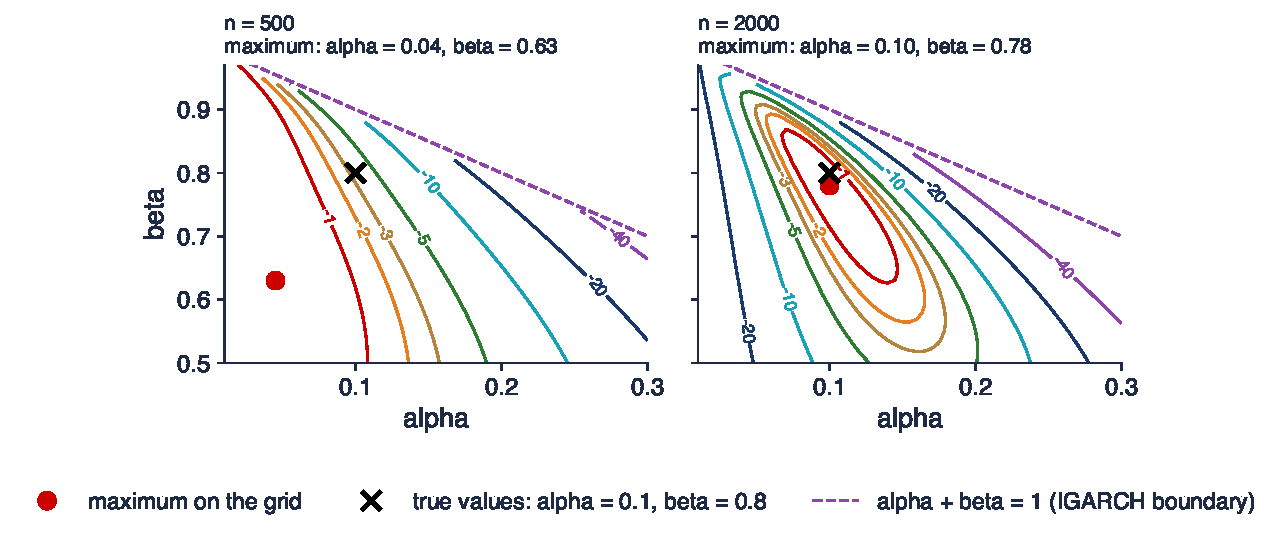
\includegraphics[width=0.97\textwidth,height=0.54\textheight,keepaspectratio]{tsa_ch5_lik_garch.pdf}
\end{center}
\vspace{-0.25cm}
\begin{itemize}
    \item GARCH(1,1) simulat cu $\omega = 0{,}1$, $\alpha = 0{,}1$, $\beta = 0{,}8$; $\omega$ fixat astfel încît varianța necondiționată să fie egală cu varianța de selecție; contururi: log-verosimilitatea minus maximul ei
    \item $n = 500$: maximul în $(0{,}04; 0{,}63)$, departe de valorile adevărate; $n = 2000$: $(0{,}10; 0{,}78)$
    \item Interpretare: o creastă lungă și plată, de-a lungul căreia $\alpha$ și $\beta$ se compensează: GARCH are nevoie de eșantioane lungi
\end{itemize}
\quantlet{TSA\_ch5\_simulation\_likelihood}{\qlurl{TSA_ch5_simulation_likelihood}}
\end{frame}

\begin{frame}{Estimarea pas cu pas și cu pachetul \texttt{arch}}
\itemsize{\footnotesize}
\begin{center}
\footnotesize
\begin{tabular}{lrrrr}
\toprule
S\&P 500, GARCH(1,1)-N & pas cu pas (SE) & \texttt{arch} & SE clasică & SE robustă \\
\midrule
$\mu$ & $0{,}0614$ ($0{,}0098$) & $0{,}0615$ & $0{,}0098$ & $0{,}0100$ \\
$\omega$ & $0{,}0253$ ($0{,}0030$) & $0{,}0254$ & $0{,}0030$ & $0{,}0048$ \\
$\alpha$ & $0{,}1205$ ($0{,}0086$) & $0{,}1206$ & $0{,}0086$ & $0{,}0118$ \\
$\beta$ & $0{,}8600$ ($0{,}0091$) & $0{,}8599$ & $0{,}0091$ & $0{,}0125$ \\
\bottomrule
\end{tabular}
\end{center}
\begin{itemize}
    \item Pas cu pas: $-\ell(\theta)$ scrisă în Python și minimizată cu \texttt{scipy.optimize.minimize}, cu restricția $\alpha + \beta < 1$
    \begin{itemize}
        \item cu pachetul: \texttt{arch\_model(r, mean='Constant', vol='GARCH', p=1, q=1, dist='normal').fit()}
    \end{itemize}
    \item SE (standard error, eroarea standard) clasică: din inversa matricei hessiene (curbura lui $\ell$); robustă: validă și cînd $z_t$ nu este Normal \refBW
    \item Interpretare: aceleași estimări pe ambele căi; SE robuste sînt de circa 1{,}4 ori mai mari: cînd $z_t$ are cozi groase, SE clasice supraestimează precizia
\end{itemize}\quantlet{TSA\_ch5\_garch\_estimation}{\qlurl{TSA_ch5_garch_estimation}}
\end{frame}

\begin{frame}{Cvasi-verosimilitatea maximă și reguli practice}
\itemsize{\small}
\begin{itemize}
    \item \textbf{QMLE} (quasi-maximum likelihood estimation, estimarea prin cvasi-verosimilitate maximă): maximizăm verosimilitatea Normală chiar dacă $z_t$ nu este Normal
    \begin{itemize}
        \item estimările rămîn consistente dacă $\mu_t$ și $\sigma_t^2$ sînt corect specificate, dar doar SE robuste (de tip „sandwich”) sînt valide \refBW
    \end{itemize}
    \item Reguli practice
    \begin{itemize}
        \item randamente în \% (nu în zecimale): algoritmul de optimizare eșuează cînd $\omega$ este foarte mic; \texttt{arch} avertizează în cazul datelor prost scalate
        \item EUR/RON variază cu circa 0,3\% pe zi: estimăm pe $10\,r_t$ și convertim înapoi $\omega$ (împărțim la 100)
        \item folosim cel puțin 1000--2000 de observații zilnice; verificăm indicatorul de convergență al algoritmului
        \item o estimare pe frontieră ($\hat\alpha + \hat\beta = 1$ sau $\hat\alpha = 0$) nu are o eroare standard obișnuită: o raportăm ca atare
    \end{itemize}
\end{itemize}
\end{frame}

\begin{frame}{Inovații Student-t și t asimetrice}
\itemsize{\small}
\begin{itemize}
    \item GARCH cu $z_t$ Normale explică doar o parte din boltire: randamentele S\&P 500 au $13{,}7$, reziduurile standardizate $\hat z_t = \hat\varepsilon_t/\hat\sigma_t$ încă $4{,}7$
    \begin{itemize}
        \item cozile groase rămase trebuie să vină din distribuția lui $z_t$
    \end{itemize}
    \item \textbf{Student-t standardizată} cu $\nu > 2$ grade de libertate \refBollT
    \begin{itemize}
        \item $z_t = t_\nu\sqrt{(\nu - 2)/\nu}$ are varianța 1; coeficientul de boltire $3 + 6/(\nu - 4)$ pentru $\nu > 4$; $\nu \to \infty$: distribuția Normală
        \item $\nu$ se estimează împreună cu $(\mu, \omega, \alpha, \beta)$: \texttt{dist='t'} în \texttt{arch}
    \end{itemize}
    \item \textbf{t asimetrică} \refHansen: încă un parametru $\lambda \in (-1, 1)$; $\lambda < 0$: o coadă stîngă mai lungă (\texttt{dist='skewt'})
    \begin{itemize}
        \item modele incluse unul în altul: Normal $\subset$ t $\subset$ t asimetrică; le comparăm prin teste LR (likelihood ratio, raportul de verosimilitate) sau prin AIC/BIC
    \end{itemize}
\end{itemize}
\end{frame}

\begin{frame}{S\&P 500: trei distribuții ale inovațiilor}
\itemsize{\footnotesize}
\begin{center}
\footnotesize
\begin{tabular}{lrrrrrrr}
\toprule
GARCH(1,1) & $\omega$ & $\alpha$ & $\beta$ & $\nu$ & $\lambda$ & log-verosim. & $\alpha + \beta$ \\
\midrule
Normală & $0{,}0254$ & $0{,}121$ & $0{,}860$ & -- & -- & $\ensuremath{-}9218{,}0$ & $0{,}980$ \\
Student-t & $0{,}0157$ & $0{,}123$ & $0{,}872$ & $6{,}26$ & -- & $\ensuremath{-}9062{,}5$ & $0{,}995$ \\
t asimetrică & $0{,}0153$ & $0{,}120$ & $0{,}872$ & $6{,}92$ & $\ensuremath{-}0{,}114$ & $\ensuremath{-}9038{,}4$ & $0{,}993$ \\
\bottomrule
\end{tabular}
\end{center}
\begin{itemize}
    \item Statistica LR $2(\ell_1 - \ell_0)$, $\ell_1$ și $\ell_0$: log-verosimilitățile modelului mai mare și ale celui mai mic: t față de Normal $311{,}0$ (o restricție, $\chi^2_{0{,}95}(1) = 3{,}84$); t asimetrică față de t $48{,}1$: ambele resping modelul mai mic
    \item $\hat\nu = 6{,}26$: cozi mult mai groase decît la distribuția Normală; $\hat\lambda = \ensuremath{-}0{,}114$: scăderile mari sînt mai frecvente decît creșterile mari
    \item Interpretare: $\alpha$ și $\beta$ aproape nu se schimbă; distribuția inovațiilor contează pentru cuantilele din coadă (VaR), mai puțin pentru $\sigma_t$
\end{itemize}\quantlet{TSA\_ch5\_garch\_estimation}{\qlurl{TSA_ch5_garch_estimation}}
\end{frame}

\begin{frame}{Graficele QQ ale reziduurilor standardizate}
\itemsize{\footnotesize}
\begin{center}
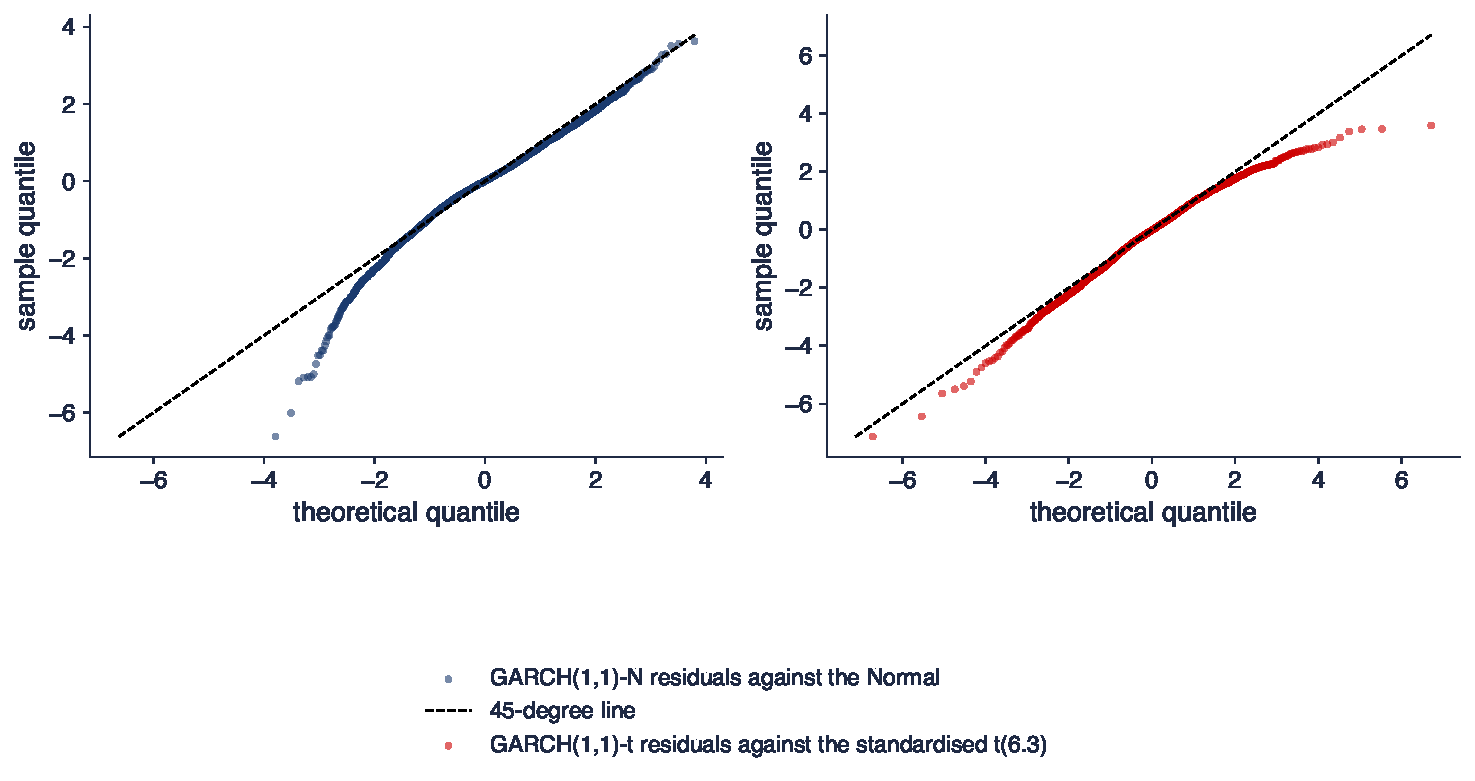
\includegraphics[width=0.97\textwidth,height=0.54\textheight,keepaspectratio]{tsa_ch5_qq.pdf}
\end{center}
\vspace{-0.25cm}
\begin{itemize}
    \item Graficul QQ (quantile--quantile): cuantilele de selecție ale lui $\hat z_t$ față de cuantilele distribuției presupuse; o dreaptă înseamnă o potrivire bună
    \item Stînga, GARCH-N față de distribuția Normală: cuantila de 0,1\% este $\ensuremath{-}4{,}81$, față de $\ensuremath{-}3{,}09$ teoretic; dreapta, GARCH-t față de t standardizată ($\hat\nu = 6{,}3$): $\ensuremath{-}4{,}79$ față de $\ensuremath{-}4{,}19$
    \item Interpretare: distribuția t se potrivește mult mai bine, dar cele mai mari scăderi sînt tot mai adînci: problema este coada stîngă (asimetria, secțiunea 7)
\end{itemize}
\quantlet{TSA\_ch5\_garch\_estimation}{\qlurl{TSA_ch5_garch_estimation}}
\end{frame}

\begin{frame}{Recapitulare: estimarea prin verosimilitate maximă}
\itemsize{\small}
\begin{itemize}
    \item $\ell(\theta)$ = suma log-densităților condiționate; $\sigma_t^2(\theta)$ calculat recursiv; maximizare numerică
    \item Verosimilitatea are o creastă în $(\alpha, \beta)$: eșantioane lungi; raportăm SE robuste
    \item Inovații Student-t sau t asimetrice pentru cozile groase rămase
\end{itemize}
\end{frame}


%=============================================================================
\section{GARCH pe patru piețe și modele ARMA-GARCH}
%=============================================================================

\begin{frame}{Estimările GARCH(1,1)-t}
\itemsize{\footnotesize}
\begin{center}
\scriptsize
\begin{tabular}{lrrrrrrrrr}
\toprule
& din & $\omega$ & $\alpha$ & $\beta$ & $\nu$ & $\alpha + \beta$ & înjumătățire & vol. lungă durată & vol. selecție \\
\midrule
S\&P 500 & 2000 & $0{,}0157$ & $0{,}123$ & $0{,}872$ & $6{,}26$ & $0{,}995$ & 131 & 27{,}3 & 19{,}2 \\
BET & 2000 & $0{,}0448$ & $0{,}192$ & $0{,}799$ & $5{,}01$ & $0{,}991$ & 74 & 34{,}7 & 22{,}1 \\
EUR/RON & 2005 & $0{,}0000$ & $0{,}123$ & $0{,}877$ & $4{,}20$ & $1{,}000$ & -- & -- & 4{,}4 \\
Bitcoin & 2014 & $0{,}1937$ & $0{,}109$ & $0{,}891$ & $3{,}18$ & $1{,}000$ & -- & -- & 66{,}6 \\
\bottomrule
\end{tabular}
\end{center}
\begin{itemize}
    \item Randamente logaritmice zilnice în \% pînă la 18 septembrie 2026; timpul de înjumătățire în zile; volatilitățile anualizate cu numărul efectiv de observații pe an (Bitcoin: 365), în \%
    \item S\&P 500 și BET: $\alpha + \beta$ egal cu 0{,}995 și 0{,}991, timpi de înjumătățire de 131 și 74 de zile de tranzacționare; BET reacționează mai puternic la știri ($\alpha = 0{,}192$)
    \item EUR/RON și Bitcoin: $\hat\alpha + \hat\beta = 1$, pe frontieră: IGARCH; toate valorile $\hat\nu$ între 3{,}18 și 6{,}26: cozi groase peste tot
\end{itemize}\quantlet{TSA\_ch5\_volatility\_markets}{\qlurl{TSA_ch5_volatility_markets}}
\end{frame}

\begin{frame}{Interpretarea IGARCH și a volatilității de lungă durată}
\itemsize{\small}
\begin{itemize}
    \item EUR/RON: $\hat\omega \approx 0$ și $\hat\beta = 0{,}88$: un EWMA cu $\lambda \approx 0{,}88$; Bitcoin: $\hat\beta = 0{,}89$
    \begin{itemize}
        \item nu există timp de înjumătățire și nici volatilitate de lungă durată: nivelul volatilității se deplasează ca un mers aleator (\tsachlink{https://danpele.github.io/Time-Series-Analysis/RO/Cursuri/capitol3_radacini_unitare_modele_arima.pdf}{Capitolul 3})
        \item EUR/RON: un curs în regim de managed float, a cărui volatilitate a scăzut de la un regim la altul (politica BNR se schimbă în timp)
    \end{itemize}
    \item \textbf{Întrebare pentru sală}: S\&P 500: volatilitatea de lungă durată 27{,}3\%, volatilitatea de selecție 19{,}2\%. Este greșit modelul?
    \begin{itemize}
        \item \textbf{Răspuns}: nu neapărat: $\bar\sigma^2 = \omega/(1 - \alpha - \beta)$ se împarte la $1 - \alpha - \beta = 0{,}0053$, un număr mic și imprecis
        \item GARCH cu inovații Normale dă 18{,}1\%: nivelul de lungă durată este cel mai puțin sigur rezultat al unui GARCH persistent
    \end{itemize}
\end{itemize}
\end{frame}

\begin{frame}{Volatilitatea condiționată: S\&P 500 și BET}
\itemsize{\footnotesize}
\begin{center}
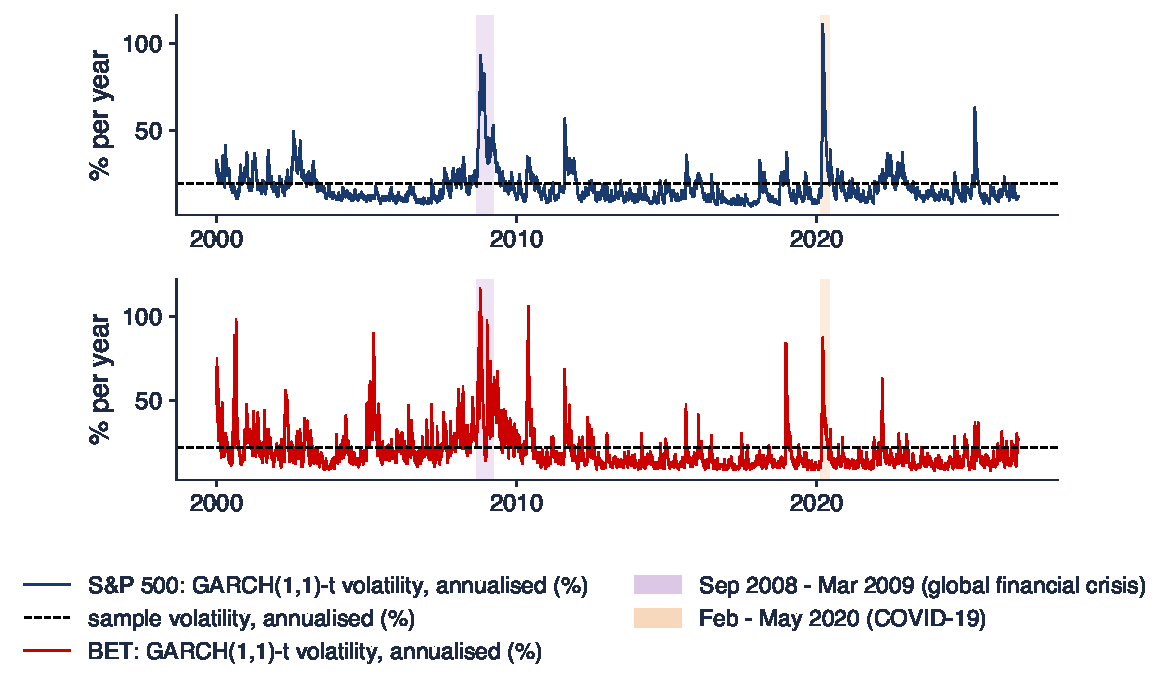
\includegraphics[width=0.97\textwidth,height=0.62\textheight,keepaspectratio]{tsa_ch5_vol_sp500_bet.pdf}
\end{center}
\vspace{-0.25cm}
\begin{itemize}
    \item Volatilitatea GARCH(1,1)-t $\hat\sigma_t$, anualizată; linia întreruptă: volatilitatea de selecție
    \item S\&P 500: vîrfuri de 93\% (16 octombrie 2008) și 111\% (17 martie 2020); BET: 117\% (15 octombrie 2008) și 88\% (18 martie 2020); medianele 14{,}3\% și 15{,}6\%
\end{itemize}
\quantlet{TSA\_ch5\_volatility\_markets}{\qlurl{TSA_ch5_volatility_markets}}
\end{frame}

\begin{frame}{Volatilitatea condiționată: EUR/RON și Bitcoin}
\itemsize{\footnotesize}
\begin{center}
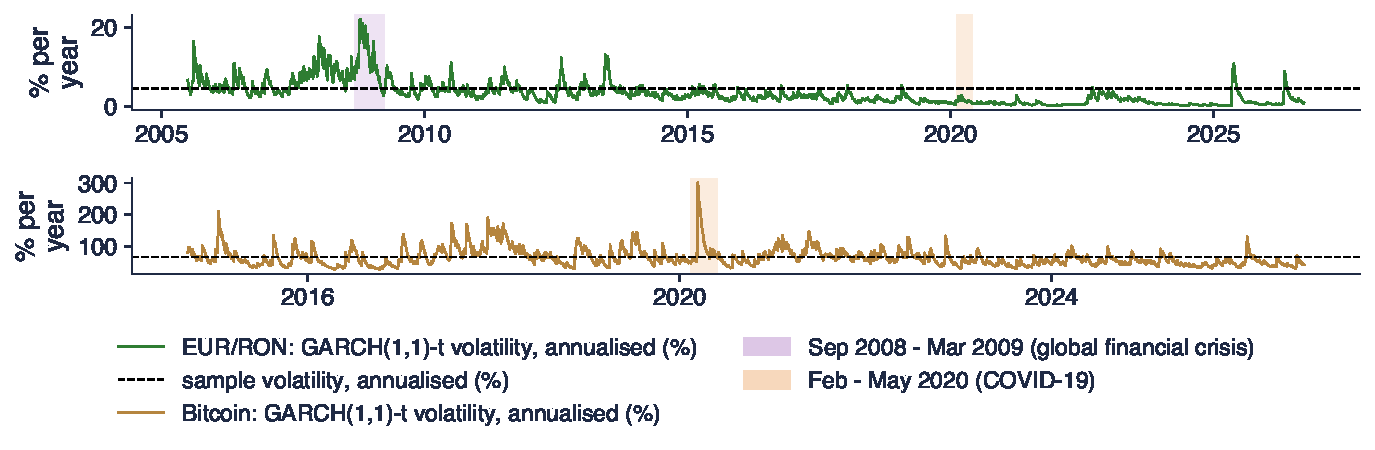
\includegraphics[width=0.97\textwidth,height=0.60\textheight,keepaspectratio]{tsa_ch5_vol_eurron_btc.pdf}
\end{center}
\vspace{-0.25cm}
\begin{itemize}
    \item EUR/RON: 22\% în vîrful crizei din 2008 (13 octombrie 2008), doar 3\% în 2020; la 18 septembrie 2026: 1{,}0\%
    \item Bitcoin: 301\% pe 13 martie 2020; mediana 58{,}7\%, de 4{,}1 ori mai mare decît mediana S\&P 500
    \item Interpretare: cele două serii IGARCH au niveluri de volatilitate care se deplasează: nu există un singur nivel „normal”
\end{itemize}
\quantlet{TSA\_ch5\_volatility\_markets}{\qlurl{TSA_ch5_volatility_markets}}
\end{frame}

\begin{frame}{Durata unui șoc de volatilitate}
\itemsize{\footnotesize}
\begin{center}
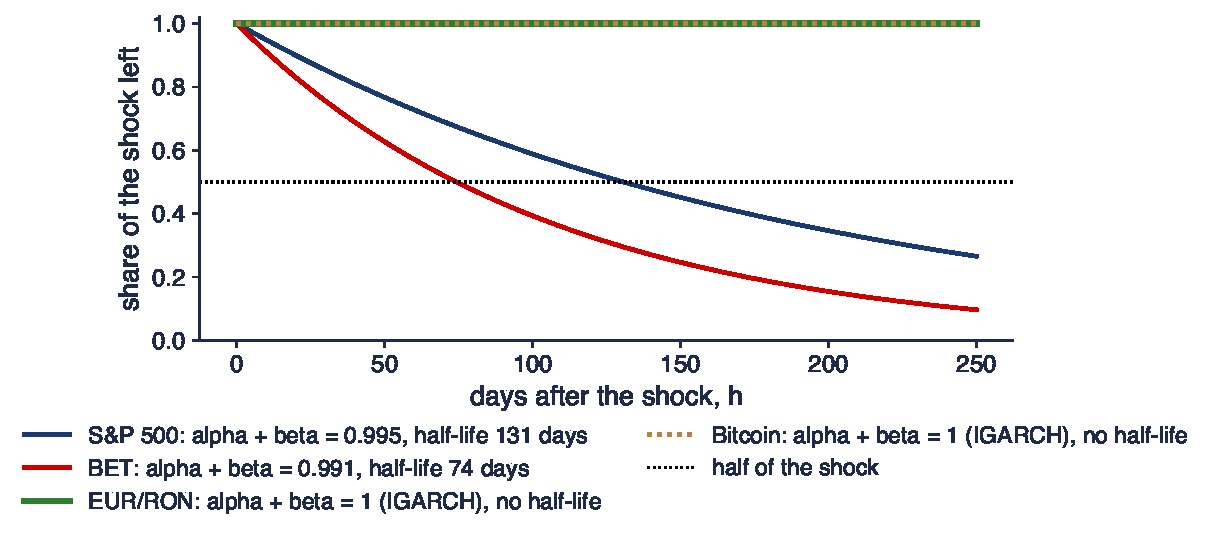
\includegraphics[width=0.97\textwidth,height=0.58\textheight,keepaspectratio]{tsa_ch5_persistence.pdf}
\end{center}
\vspace{-0.25cm}
\begin{itemize}
    \item Ponderea unui șoc de varianță rămasă după $h$ zile: $(\alpha + \beta)^h$; timpul de înjumătățire este punctul în care curba trece de 1/2
    \item Interpretare: după o criză, S\&P 500 are nevoie de circa jumătate de an ca să înjumătățească varianța în exces, BET de circa trei luni; EUR/RON și Bitcoin, niciodată
\end{itemize}
\quantlet{TSA\_ch5\_volatility\_markets}{\qlurl{TSA_ch5_volatility_markets}}
\end{frame}

\begin{frame}{ARMA-GARCH: un model pentru medie și varianță}
\itemsize{\small}
\begin{itemize}
    \item \textbf{ARMA($p$,$q$)-GARCH(1,1)}: $r_t = c + \sum_{i=1}^{p}\phi_i r_{t-i} + \varepsilon_t + \sum_{j=1}^{q}\theta_j\varepsilon_{t-j}$, \quad $\varepsilon_t = \sigma_t z_t$, \quad $\sigma_t^2 = \omega + \alpha\varepsilon_{t-1}^2 + \beta\sigma_{t-1}^2$
    \begin{itemize}
        \item partea ARMA este modelul din \tsachlink{https://danpele.github.io/Time-Series-Analysis/RO/Cursuri/capitol2_modele_arma.pdf}{Capitolul 2}; erorile lui nu mai sînt i.i.d., ci urmează un GARCH
    \end{itemize}
    \item Estimarea: ambele părți simultan, prin verosimilitate maximă
    \begin{itemize}
        \item în \texttt{arch}: \texttt{arch\_model(r, mean='AR', lags=1, vol='GARCH', dist='t')} (doar medii AR; pentru termeni MA, două etape sau alt pachet)
    \end{itemize}
    \item Limitele estimării în doi pași (OLS pentru medie, apoi GARCH)
    \begin{itemize}
        \item coeficienții OLS rămîn consistenți, dar SE obișnuite presupun o varianță constantă: testele $t$ din \tsachlink{https://danpele.github.io/Time-Series-Analysis/RO/Cursuri/capitol2_modele_arma.pdf}{Capitolul 2} sînt greșite
        \item estimarea comună prin verosimilitate maximă dă o pondere mai mică zilelor agitate, deci un $\hat\phi$ mai precis și intervale valide
    \end{itemize}
\end{itemize}
\end{frame}

\begin{frame}{AR(1)-GARCH(1,1)-t pe patru serii}
\itemsize{\footnotesize}
\begin{center}
\scriptsize
\begin{tabular}{lrrrrrr}
\toprule
& $p$ (BIC) & $\hat\phi$, OLS (SE) & $\hat\phi$, AR-GARCH (SE) & $Q(10)$ al $\hat z_t$, medie const. & $Q(10)$ al $\hat z_t$, AR(1) & $\Delta$BIC \\
\midrule
S\&P 500 & 1 & $\ensuremath{-}0{,}099$ ($0{,}012$) & $\ensuremath{-}0{,}054$ ($0{,}012$) & $21{,}9$ (0{,}016) & $15{,}1$ (0{,}087) & ${\ensuremath{-}19{,}5}$ \\
BET & 1 & $0{,}109$ ($0{,}012$) & $0{,}091$ ($0{,}013$) & $114{,}6$ ($<$\,0{,}001) & $28{,}6$ ($<$\,0{,}001) & ${\ensuremath{-}46{,}9}$ \\
EUR/RON & 3 & $0{,}170$ ($0{,}013$) & $0{,}031$ ($0{,}016$) & $10{,}5$ (0{,}402) & $8{,}7$ (0{,}469) & ${4{,}2}$ \\
Bitcoin & 0 & $\ensuremath{-}0{,}022$ ($0{,}015$) & $\ensuremath{-}0{,}043$ ($0{,}014$) & $29{,}9$ ($<$\,0{,}001) & $48{,}4$ ($<$\,0{,}001) & ${\ensuremath{-}9{,}5}$ \\
\bottomrule
\end{tabular}
\end{center}
\begin{itemize}
    \item $p$: ordinul AR ales după BIC cu varianță constantă; SE pentru AR-GARCH: robuste; $\Delta$BIC: AR(1)-GARCH-t minus GARCH-t cu medie constantă (negativ: se preferă AR(1))
    \item S\&P 500: $\hat\phi$ scade de la \ensuremath{-}0{,}099 la \ensuremath{-}0{,}054: valoarea OLS reflectă mai ales zilele agitate din 2008 și 2020
    \item BET: autocorelația pozitivă se menține ($\hat\phi = 0{,}091$, $t = 6{,}8$): ajustarea lentă a prețurilor pe o piață mai puțin lichidă; EUR/RON: de la 0{,}170 la 0{,}031, nu mai este semnificativ
    \item Interpretare: modelul pentru medie și cel pentru varianță trebuie alese împreună; concluziile despre $\phi$ se pot schimba
\end{itemize}\quantlet{TSA\_ch5\_arma\_garch}{\qlurl{TSA_ch5_arma_garch}}
\end{frame}

\begin{frame}{Intervale de prognoză variabile în timp}
\itemsize{\footnotesize}
\begin{center}
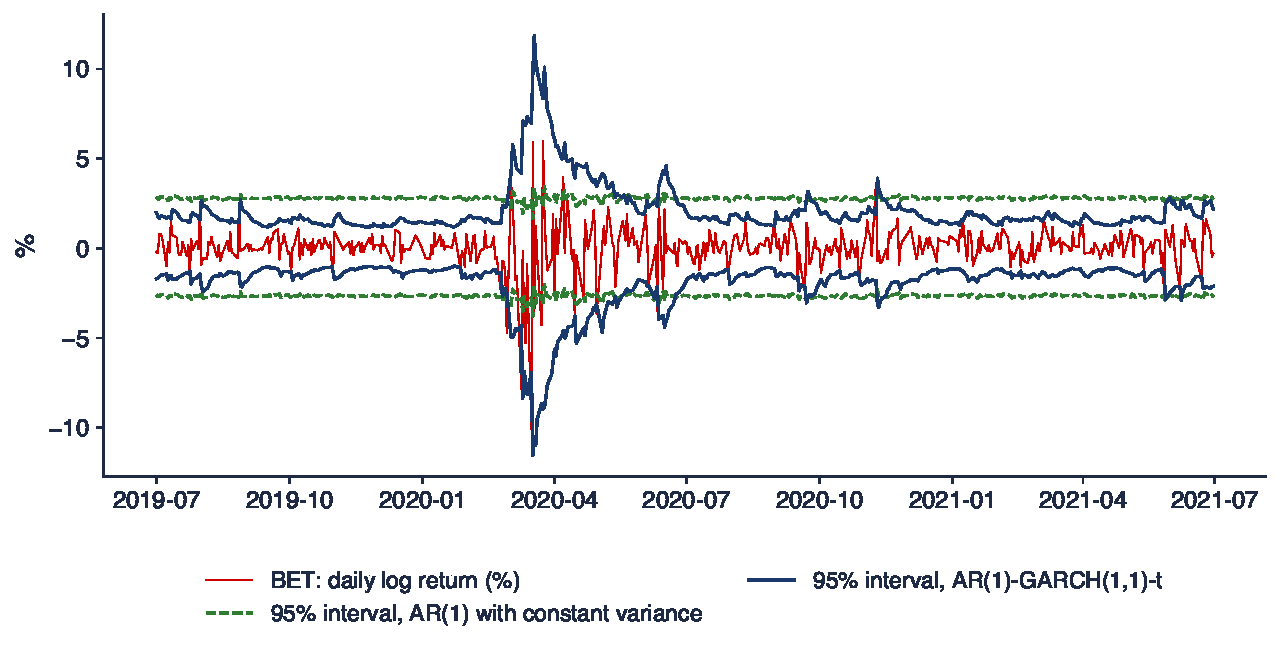
\includegraphics[width=0.97\textwidth,height=0.60\textheight,keepaspectratio]{tsa_ch5_bands.pdf}
\end{center}
\vspace{-0.25cm}
\begin{itemize}
    \item BET, intervale de 95\% cu o zi înainte: AR(1) cu varianță constantă (lățimea de 5{,}4 puncte în fiecare zi) și AR(1)-GARCH(1,1)-t (lățimea de la 2{,}2 la 22{,}5 puncte în această fereastră)
\end{itemize}
\quantlet{TSA\_ch5\_arma\_garch}{\qlurl{TSA_ch5_arma_garch}}
\end{frame}

\begin{frame}{Interpretarea celor două intervale}
\itemsize{\small}
\begin{itemize}
    \item Pe întregul eșantion ambele ratează circa 5\% dintre zile: 5{,}0\% și 5{,}2\%
    \begin{itemize}
        \item intervalul constant este corect în medie, dar greșit aproape în fiecare zi
    \end{itemize}
    \item În 2017 (an liniștit): intervalul constant ratează 0{,}4\% dintre zile, intervalul GARCH 2{,}0\%
    \begin{itemize}
        \item în martie--aprilie 2020: 33{,}3\% față de 9{,}5\%: ratările intervalului constant se grupează în crize
    \end{itemize}
    \item \tsachlink{https://danpele.github.io/Time-Series-Analysis/RO/Cursuri/capitol2_modele_arma.pdf}{Capitolul 2} a dat intervale a căror lățime depinde doar de orizont; cu GARCH ea depinde și de starea curentă
\end{itemize}
\end{frame}

\begin{frame}{Recapitulare: patru piețe și ARMA-GARCH}
\itemsize{\small}
\begin{itemize}
    \item $\alpha + \beta$ apropiat de 1 peste tot; EUR/RON și Bitcoin sînt IGARCH
    \item Volatilitatea de lungă durată este imprecisă cînd $\alpha + \beta$ este aproape de 1
    \item ARMA-GARCH: media din \tsachlink{https://danpele.github.io/Time-Series-Analysis/RO/Cursuri/capitol2_modele_arma.pdf}{Capitolul 2} cu erori GARCH; MLE comun; intervale care urmează volatilitatea
\end{itemize}
\end{frame}


%=============================================================================
\section{Asimetria și efectul de levier}
%=============================================================================

\begin{frame}{Efectul de levier și curba de impact a știrilor}
\itemsize{\small}
\begin{itemize}
    \item \textbf{Efectul de levier}: scăderile prețurilor acțiunilor cresc volatilitatea mai mult decît creșterile de aceeași mărime \refChristie
    \begin{itemize}
        \item un preț mai mic al acțiunii crește raportul datorii/capitaluri proprii, deci acțiunea devine mai riscantă; știrile despre un risc mai mare scad și ele imediat prețurile
    \end{itemize}
    \item GARCH(1,1) nu îl poate surprinde: $\sigma_t^2$ depinde de $\varepsilon_{t-1}^2$, nu de semnul lui $\varepsilon_{t-1}$
    \begin{itemize}
        \item graficul QQ și t asimetrică ($\hat\lambda < 0$) au arătat deja spre coada stîngă
    \end{itemize}
    \item \textbf{NIC} (news impact curve, curba de impact a știrilor) \refEN: $\sigma_t^2$ ca funcție de $\varepsilon_{t-1}$, cu $\sigma_{t-1}^2$ fixat la varianța necondiționată; pentru GARCH, o parabolă simetrică
\end{itemize}
\end{frame}

\begin{frame}{GJR-GARCH și EGARCH}
\itemsize{\small}
\begin{itemize}
    \item \textbf{GJR-GARCH} \refGJR: $\sigma_t^2 = \omega + (\alpha + \gamma\,I_{t-1})\,\varepsilon_{t-1}^2 + \beta\sigma_{t-1}^2$, cu $I_{t-1} = 1$ dacă $\varepsilon_{t-1} < 0$, altfel 0
    \begin{itemize}
        \item știri bune: panta $\alpha$; știri proaste: $\alpha + \gamma$; efect de levier: $\gamma > 0$; în \texttt{arch}: \texttt{o=1}
        \item persistența $\alpha + \beta + \gamma/2$ pentru $z_t$ simetric (jumătate dintre șocuri sînt negative)
    \end{itemize}
    \item \textbf{EGARCH} (exponential GARCH, GARCH exponențial) \refNelson: $\ln\sigma_t^2 = \omega + \alpha\big(|z_{t-1}| - E|z_{t-1}|\big) + \gamma z_{t-1} + \beta\ln\sigma_{t-1}^2$
    \begin{itemize}
        \item $z_{t-1}$: șocul standardizat de ieri; $E|z_{t-1}|$: valoarea lui absolută medie ($\sqrt{2/\pi}$ pentru distribuția Normală); $\alpha$: efectul mărimii; $\gamma$: efectul semnului
        \item logaritmul păstrează $\sigma_t^2 > 0$ fără restricții de semn; efect de levier: $\gamma < 0$; persistența: $\beta$
    \end{itemize}
    \item Ambele au un parametru în plus față de GARCH(1,1); testăm $\gamma = 0$ cu statistica $t$ sau cu un test LR, $\chi^2(1)$
\end{itemize}
\end{frame}

\begin{frame}{Curbele de impact ale știrilor: S\&P 500 și Bitcoin}
\itemsize{\footnotesize}
\begin{center}
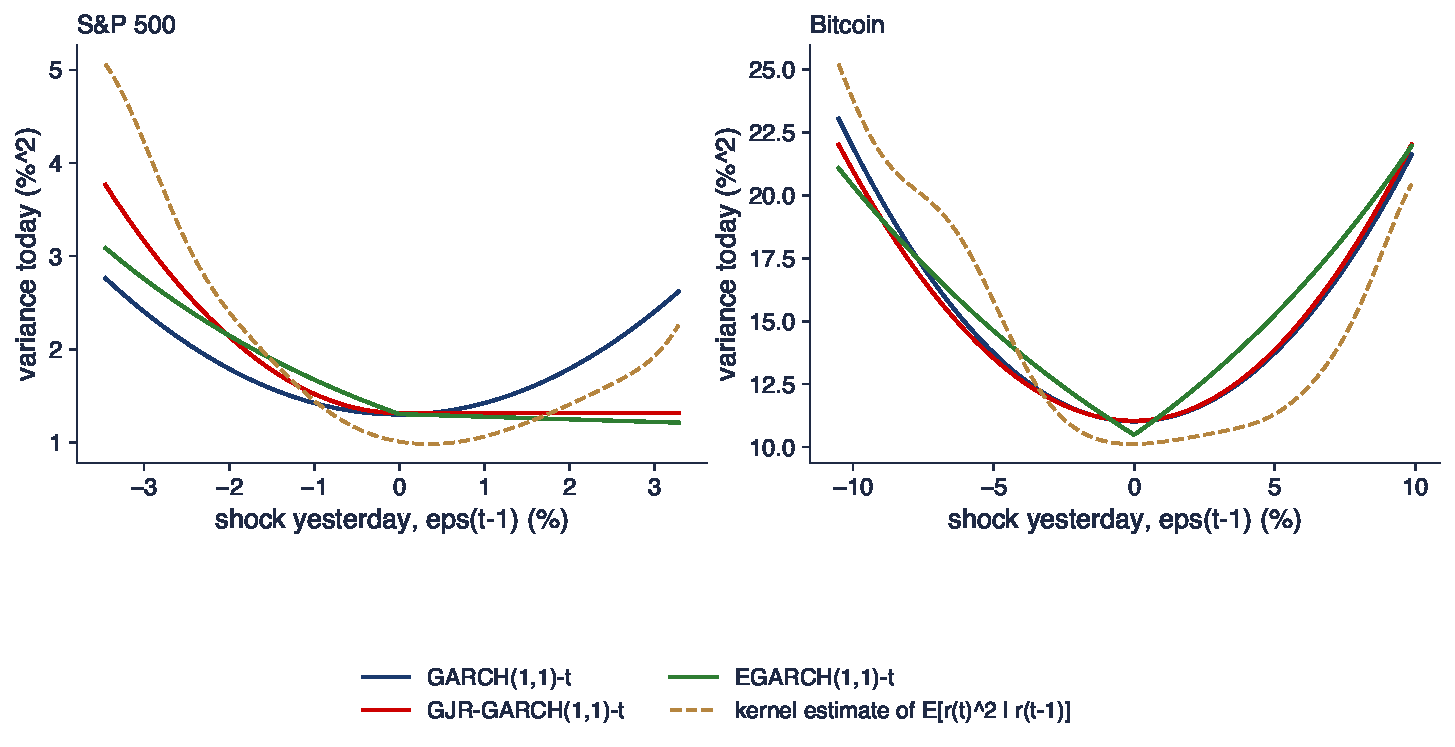
\includegraphics[width=0.97\textwidth,height=0.62\textheight,keepaspectratio]{tsa_ch5_nic.pdf}
\end{center}
\vspace{-0.25cm}
\begin{itemize}
    \item Curbele modelelor: $\sigma_t^2$ în funcție de $\varepsilon_{t-1}$, cu $\sigma_{t-1}^2$ la varianța de selecție; linia întreruptă: o estimare nucleu (Nadaraya--Watson) a lui $E[r_t^2 \mid r_{t-1}]$, fără model
    \item S\&P 500, GJR: după o scădere de 2\%, varianța de mîine este de 1{,}62 ori mai mare decît după o creștere de 2\%; Bitcoin: raportul 1{,}00, o curbă simetrică
\end{itemize}
\quantlet{TSA\_ch5\_asymmetry}{\qlurl{TSA_ch5_asymmetry}}
\end{frame}

\begin{frame}{Asimetria pe patru piețe}
\itemsize{\footnotesize}
\begin{center}
\scriptsize
\begin{tabular}{lrrrrrrrr}
\toprule
& GJR $\alpha$ & GJR $\gamma$ & $t(\gamma)$ & LR & p & $\Delta$BIC & EGARCH $\gamma$ & $t(\gamma)$ \\
\midrule
S\&P 500 & $0{,}000$ & $0{,}205$ & $10{,}0$ & $235{,}7$ & $<$\,0{,}001 & ${\ensuremath{-}226{,}8}$ & ${\ensuremath{-}0{,}165}$ & ${\ensuremath{-}15{,}2}$ \\
BET & $0{,}172$ & $0{,}043$ & $2{,}1$ & $4{,}9$ & 0{,}026 & ${3{,}9}$ & ${\ensuremath{-}0{,}028}$ & ${\ensuremath{-}2{,}6}$ \\
EUR/RON & $0{,}103$ & $0{,}039$ & $3{,}0$ & $9{,}3$ & 0{,}002 & ${\ensuremath{-}0{,}7}$ & ${\ensuremath{-}0{,}040}$ & ${\ensuremath{-}2{,}5}$ \\
Bitcoin & $0{,}113$ & $\ensuremath{-}0{,}013$ & $\ensuremath{-}0{,}7$ & $0{,}7$ & 0{,}416 & ${7{,}7}$ & ${0{,}015}$ & ${1{,}2}$ \\
\bottomrule
\end{tabular}
\end{center}
\begin{itemize}
    \item Inovații Student-t; statistici $t$ robuste; LR $= 2(\ell_{GJR} - \ell_{GARCH}) \sim \chi^2(1)$; $\Delta$BIC: GJR minus GARCH (negativ: se preferă GJR)
    \item S\&P 500: GJR $\hat\alpha = 0{,}000$: doar știrile proaste cresc volatilitatea; un efect de levier foarte puternic
    \item BET: slab, semnificativ după LR, dar BIC preferă GARCH; Bitcoin: niciun efect; EUR/RON: $r_t > 0$ înseamnă un leu mai slab, deci „știrile proaste” din GJR sînt zilele în care leul se întărește
    \item Interpretare: efectul de levier este o proprietate a piețelor mature de acțiuni, nu a oricărei serii financiare
\end{itemize}\quantlet{TSA\_ch5\_asymmetry}{\qlurl{TSA_ch5_asymmetry}}
\end{frame}

\begin{frame}{Recapitulare: asimetria}
\itemsize{\small}
\begin{itemize}
    \item GJR: o pantă suplimentară $\gamma$ pentru șocurile negative; EGARCH: un termen de semn $\gamma z_{t-1}$ în $\ln\sigma_t^2$
    \item Curba de impact a știrilor arată asimetria dintr-o privire
    \item Puternică la S\&P 500, slabă la BET, absentă la Bitcoin
\end{itemize}
\end{frame}


%=============================================================================
\section{Diagnosticare și alegerea modelului}
%=============================================================================

\begin{frame}{Verificarea unui model estimat}
\itemsize{\small}
\begin{itemize}
    \item Dacă modelul este corect, \textbf{reziduurile standardizate} $\hat z_t = (r_t - \hat\mu_t)/\hat\sigma_t$ sînt aproape i.i.d., cu media 0 și varianța 1
    \begin{itemize}
        \item Ljung--Box $Q(10)$ pe $\hat z_t$: nu a rămas autocorelație în medie (verificarea din \tsachlink{https://danpele.github.io/Time-Series-Analysis/RO/Cursuri/capitol2_modele_arma.pdf}{Capitolul 2})
        \item Ljung--Box $Q(10)$ pe $\hat z_t^2$ și ARCH-LM pe $\hat z_t$: nu au rămas efecte ARCH
        \item graficul QQ al lui $\hat z_t$: este corectă distribuția presupusă?
    \end{itemize}
    \item \textbf{Testul de asimetrie (sign bias)} \refEN: regresia lui $\hat z_t^2$ pe $I_{t-1}$, $I_{t-1}\hat\varepsilon_{t-1}$ și $(1 - I_{t-1})\hat\varepsilon_{t-1}$
    \begin{itemize}
        \item testul comun $T R^2 \sim \chi^2(3)$: o respingere înseamnă că semnul șocurilor trecute încă anticipează varianța
    \end{itemize}
    \item Un diagnostic trecut nu dovedește că modelul este corect; unul picat arată unde greșește
\end{itemize}
\end{frame}

\begin{frame}{Autocorelațiile eliminate de GARCH}
\itemsize{\footnotesize}
\begin{center}
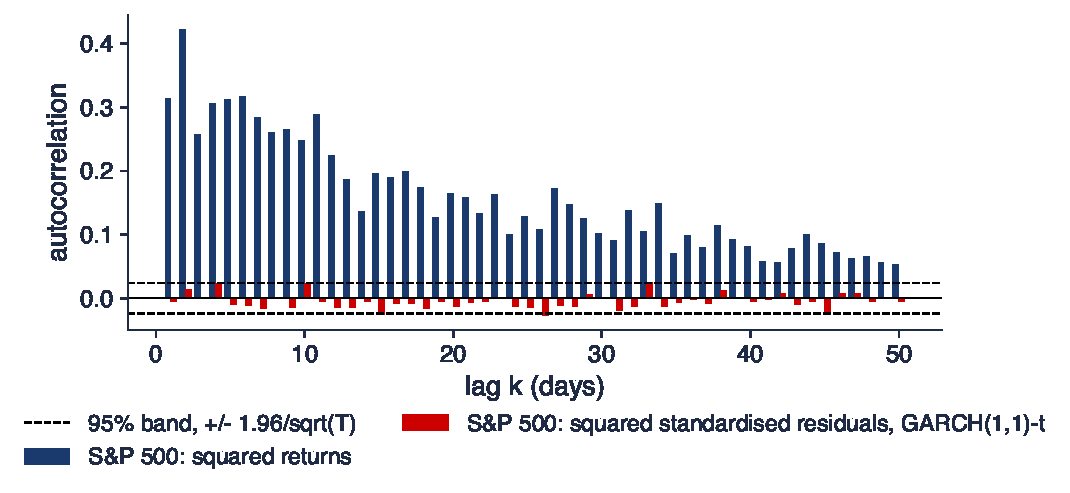
\includegraphics[width=0.97\textwidth,height=0.56\textheight,keepaspectratio]{tsa_ch5_acf_diag.pdf}
\end{center}
\vspace{-0.25cm}
\begin{itemize}
    \item S\&P 500: ACF a lui $r_t^2$: $0{,}31$ la lagul 1, încă $0{,}053$ la lagul 50; ACF a lui $\hat z_t^2$ (GARCH(1,1)-t): $\ensuremath{-}0{,}005$ la lagul 1, cel mult $0{,}028$ în valoare absolută; banda $\pm0{,}024$
    \item Interpretare: patru parametri absorb aproape tot volatility clustering din 27 de ani de date zilnice
\end{itemize}
\quantlet{TSA\_ch5\_diagnostics}{\qlurl{TSA_ch5_diagnostics}}
\end{frame}

\begin{frame}{Diagnosticare pe date reale}
\itemsize{\footnotesize}
\begin{center}
\scriptsize
\begin{tabular}{lrrr}
\toprule
S\&P 500 & $Q(10)$ (p) & $Q(10)$ al pătratelor (p) & ARCH-LM(5) (p) \\
\midrule
randamente $r_t$ & $96{,}3$ ($<$\,0{,}001) & $6133$ ($<$\,0{,}001) & $1684$ ($<$\,0{,}001) \\
$\hat z_t$, GARCH-N & $21{,}2$ (0{,}020) & $16{,}4$ (0{,}089) & $7{,}0$ (0{,}222) \\
$\hat z_t$, GARCH-t & $21{,}9$ (0{,}016) & $13{,}6$ (0{,}192) & $4{,}8$ (0{,}438) \\
\bottomrule
\end{tabular}
\end{center}
\begin{itemize}
    \item GARCH elimină efectele ARCH ($Q(10)$ al pătratelor: de la $6133$ la $13{,}6$); rămîne puțină autocorelație în medie (medie constantă; un AR(1) ajută, secțiunea 6)
    \item Testul de asimetrie pentru GARCH-t pe S\&P 500: $\chi^2(3) = 40{,}7$ (p $<$\,0{,}001): lipsește asimetria din secțiunea 7
    \item $Q(10)$ al lui $\hat z_t^2$, GARCH-t: BET 8{,}3 (p = 0{,}596), Bitcoin 4{,}7 (p = 0{,}910), EUR/RON 0{,}004: suspect de mic (slide-ul următor)
\end{itemize}\quantlet{TSA\_ch5\_diagnostics}{\qlurl{TSA_ch5_diagnostics}}
\end{frame}

\begin{frame}{Studiu de caz: EUR/RON pe 6 mai 2025}
\itemsize{\footnotesize}
\begin{columns}[T]
\begin{column}{0.62\textwidth}
\begin{itemize}
    \item În aprilie 2025, cursul de referință a variat în medie cu 0{,}0038\% pe zi: BNR a menținut leul aproape fix
    \begin{itemize}
        \item volatilitatea IGARCH a scăzut la $\hat\sigma_t = 0{,}0078\%$; apoi cursul a crescut cu 1{,}20\% (la două zile după primul tur al alegerilor prezidențiale) și cu 1{,}21\% a doua zi
    \end{itemize}
    \item Reziduul standardizat: $\hat z_t = 154$, o zi „de 154 sigma”; următorul ca mărime este 13{,}2
    \begin{itemize}
        \item $Q(10)$ al lui $\hat z_t^2$: 0{,}004 cu această zi, 19{,}2 (p = 0{,}038) fără ea: o singură valoare ascunde efectele ARCH rămase
    \end{itemize}
    \item Lecția: un curs în regim de managed float nu se formează liber pe piață; GARCH nu poate anticipa o decizie de politică; reprezentăm întotdeauna grafic $\hat z_t$ înainte de a ne baza pe un test
\end{itemize}
\end{column}
\begin{column}{0.34\textwidth}
\centering
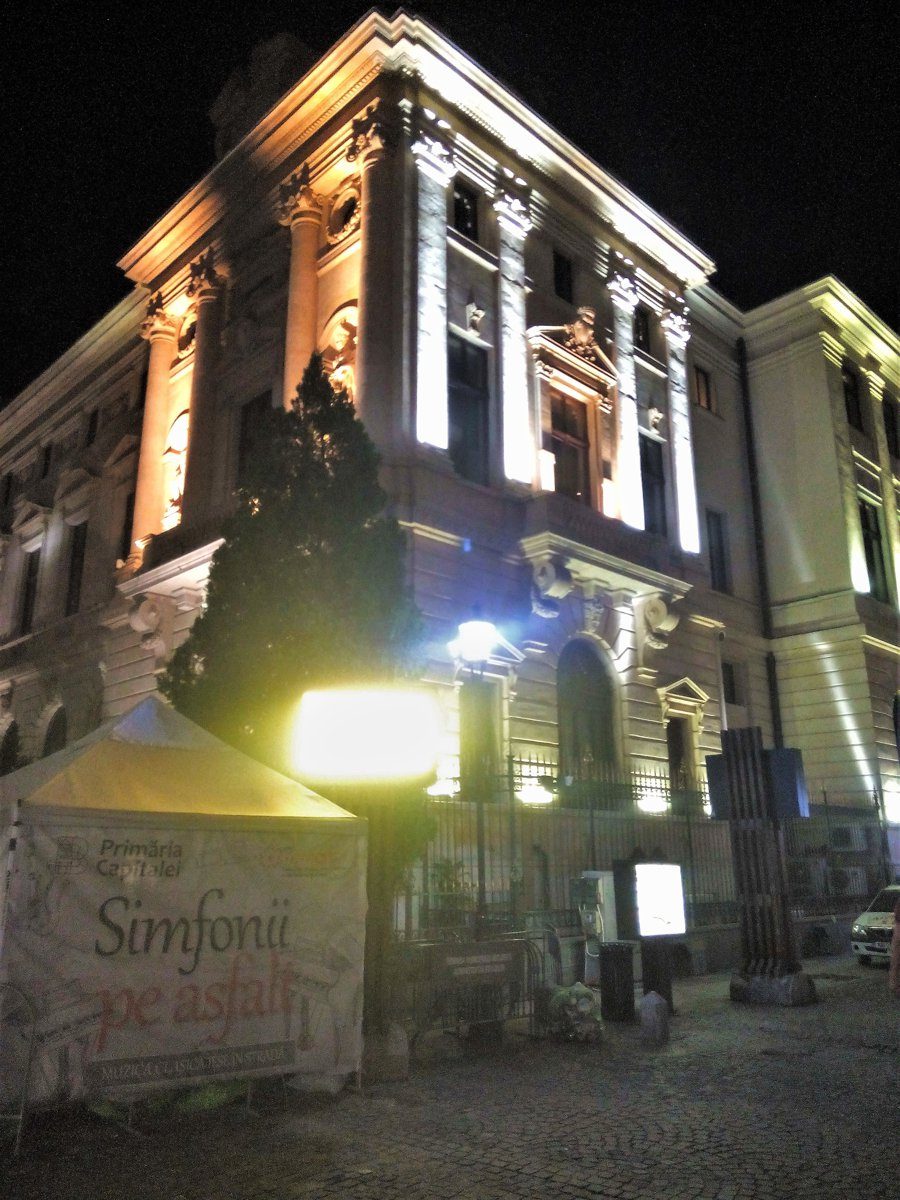
\includegraphics[height=0.28\textheight]{ch1_bnr_2018.jpg}\\[1mm]
\imgcap{Banca Națională a României, București}
\imgcredit{https://commons.wikimedia.org/wiki/File:National_Bank_of_Romania_(old_building),_Bucharest_by_nickispeaki_01.jpg}{Foto: Nickispeaki (2018); CC BY-SA 4.0; Wikimedia Commons}
\end{column}
\end{columns}
\vspace{1mm}
\quantlet{TSA\_ch5\_diagnostics}{\qlurl{TSA_ch5_diagnostics}}
\end{frame}

\begin{frame}{Nouă modele pentru S\&P 500}
\itemsize{\footnotesize}
\begin{itemize}
    \item AIC $= -2\ell + 2k$ \refAkaike; BIC $= -2\ell + k\ln T$ \refSchwarz; $k$ parametri; comparăm modele estimate pe aceleași date
\end{itemize}\begin{center}
\scriptsize
\begin{tabular}{lrrrrrr}
\toprule
& \multicolumn{2}{c}{Normală} & \multicolumn{2}{c}{Student-t} & \multicolumn{2}{c}{t asimetrică} \\ & log-verosim. & $\Delta$BIC & log-verosim. & $\Delta$BIC & log-verosim. & $\Delta$BIC \\
\midrule
GARCH(1,1) & \ensuremath{-}9218{,}0 & 648{,}9 & \ensuremath{-}9062{,}5 & 346{,}7 & \ensuremath{-}9038{,}4 & 307{,}4 \\
GJR-GARCH(1,1) & \ensuremath{-}9086{,}5 & 394{,}7 & \ensuremath{-}8944{,}6 & 119{,}9 & \ensuremath{-}8905{,}1 & 49{,}6 \\
EGARCH(1,1) & \ensuremath{-}9075{,}6 & 372{,}9 & \ensuremath{-}8922{,}1 & 74{,}8 & \ensuremath{-}8880{,}3 & 0{,}0 \\
\bottomrule
\end{tabular}
\end{center}
\begin{itemize}
    \item $\Delta$BIC: diferența față de cel mai bun model, EGARCH cu inovații t asimetrice
    \item Pornind de la GARCH Normal: doar asimetria (EGARCH Normal) reduce BIC cu 276, doar cozile groase (GARCH cu t asimetrică) cu 341, ambele cu 649
    \item Interpretare: cu 6\,714 observații, chiar și cîștigurile mici sînt „semnificative”; comparația în afara eșantionului din secțiunea 9 este testul real
\end{itemize}\quantlet{TSA\_ch5\_diagnostics}{\qlurl{TSA_ch5_diagnostics}}
\end{frame}

\begin{frame}{Recapitulare: diagnosticare și alegerea modelului}
\itemsize{\small}
\begin{itemize}
    \item Reziduurile standardizate: fără autocorelație în $\hat z_t$ și $\hat z_t^2$, distribuția potrivită, fără efect de semn
    \item Un singur $\hat z_t$ extrem poate ascunde totul: graficul înaintea testului
    \item AIC/BIC pe aceleași date; potrivirea în eșantion nu înseamnă capacitate de prognoză
\end{itemize}
\end{frame}


%=============================================================================
\section{Prognoza varianței și evaluarea ei}
%=============================================================================

\begin{frame}{Prognoze pe mai mulți pași}
\itemsize{\small}
\begin{itemize}
    \item Un pas: $\sigma_{t+1}^2 = \omega + \alpha\varepsilon_t^2 + \beta\sigma_t^2$ este cunoscut la sfîrșitul zilei $t$
    \begin{itemize}
        \item doi pași: $E_t[\sigma_{t+2}^2] = \omega + \alpha E_t[\varepsilon_{t+1}^2] + \beta\sigma_{t+1}^2 = \omega + (\alpha + \beta)\sigma_{t+1}^2$, deoarece $E_t[\varepsilon_{t+1}^2] = \sigma_{t+1}^2$
    \end{itemize}
    \item Prin inducție: $E_t[\sigma_{t+h}^2] = \bar\sigma^2 + (\alpha + \beta)^{h-1}(\sigma_{t+1}^2 - \bar\sigma^2)$
    \begin{itemize}
        \item prognoza converge spre varianța de lungă durată, așa cum prognoza unui AR(1) converge spre medie (\tsachlink{https://danpele.github.io/Time-Series-Analysis/RO/Cursuri/capitol2_modele_arma.pdf}{Capitolul 2})
    \end{itemize}
    \item Varianța randamentului pe $H$ zile: suma prognozelor zilnice (randamentele sînt necorelate)
    \begin{itemize}
        \item $\mathrm{Var}_t(r_{t+1} + \dots + r_{t+H}) = \sum_{h=1}^{H} E_t[\sigma_{t+h}^2]$, nu $H\sigma_{t+1}^2$
        \item regula rădăcinii pătrate a timpului, $\sigma_{t+1}\sqrt{H}$, dă valori prea mari în criză și prea mici într-o perioadă liniștită
    \end{itemize}
\end{itemize}
\end{frame}

\begin{frame}{Exemplu rezolvat: S\&P 500 la 18 septembrie 2026}
\itemsize{\small}
\begin{itemize}
    \item GARCH(1,1)-t: $\alpha + \beta = 0{,}9947$, $\bar\sigma^2 = 2{,}972$; prognoza pentru ziua următoare $\sigma_{t+1}^2 = 0{,}509$ (sub nivelul de lungă durată)
    \item Pas cu pas
    \begin{itemize}
        \item ziua 10: $2{,}972 + 0{,}9947^{9}(0{,}509 - 2{,}972) = 2{,}972 + 0{,}953 \times (0{,}509 - 2{,}972) = 0{,}624$
        \item varianța pe 10 zile: suma celor zece prognoze zilnice $= 5{,}67$, deci volatilitatea pe 10 zile este $2{,}38\%$
        \item regula rădăcinii pătrate a timpului: $\sqrt{10 \times 0{,}509} = 2{,}26\%$: prea mică, deoarece volatilitatea este așteptată să crească spre nivelul de lungă durată
    \end{itemize}
\end{itemize}
\end{frame}

\begin{frame}{Structura la termen a volatilității}
\itemsize{\footnotesize}
\begin{center}
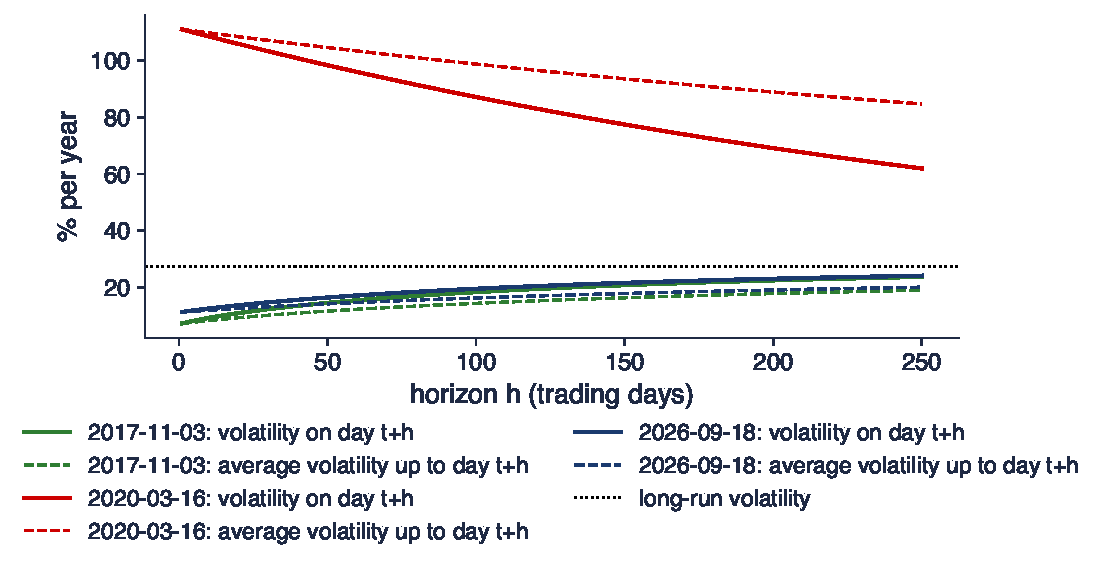
\includegraphics[width=0.97\textwidth,height=0.54\textheight,keepaspectratio]{tsa_ch5_term_structure.pdf}
\end{center}
\vspace{-0.25cm}
\begin{itemize}
    \item S\&P 500, GARCH(1,1)-t pe toate datele; prognoze făcute într-o zi liniștită (3 noiembrie 2017), în vîrful crizei COVID-19 (16 martie 2020) și la 18 septembrie 2026
    \item Ziua liniștită: 7{,}3\% mîine, în medie 19{,}0\% pe un an; vîrful COVID-19: 111{,}0\% mîine, încă 84{,}7\% în medie pe un an
    \item Interpretare: toate curbele se îndreaptă spre nivelul de lungă durată (27{,}3\%) cu aceeași viteză redusă; panta arată dacă sîntem într-o perioadă liniștită sau într-o furtună
\end{itemize}
\quantlet{TSA\_ch5\_forecasts}{\qlurl{TSA_ch5_forecasts}}
\end{frame}

\begin{frame}{Evaluarea unei prognoze de volatilitate}
\itemsize{\small}
\begin{itemize}
    \item Adevăratul $\sigma_t^2$ nu este observat niciodată: comparăm prognoza $h_t$ cu o \textbf{aproximare} zgomotoasă, aici $r_t^2$
    \begin{itemize}
        \item $E_{t-1}[r_t^2] = \sigma_t^2$ (cu $\mu \approx 0$), dar $r_t^2$ este foarte zgomotos: un $R^2$ mic chiar și pentru o prognoză perfectă \refAB
    \end{itemize}
    \item Funcția de pierdere \textbf{QLIKE} \refPatton: $L(r_t^2, h_t) = \dfrac{r_t^2}{h_t} + \ln h_t$ (pînă la o constantă); cu cît media este mai mică, cu atît mai bine
    \begin{itemize}
        \item ordonează corect prognozele chiar și cu o aproximare zgomotoasă; este minus log-verosimilitatea Normală; penalizează prognozele prea mici
    \end{itemize}
    \item \textbf{În afara eșantionului} (\tsachlink{https://danpele.github.io/Time-Series-Analysis/RO/Cursuri/capitol0_introducere.pdf}{Capitolul 0}): din 2015, fiecare prognoză folosește doar date pînă în ziua precedentă; modelele se reestimează la fiecare 250 de zile
    \item \textbf{Testul DM} \refDM: $H_0$: $E[d_t] = 0$, cu $d_t = L_t^A - L_t^B$ diferența pierderilor a două modele A și B
    \begin{itemize}
        \item $\mathrm{DM} = \bar d/\widehat{\mathrm{SE}}(\bar d)$, aproximativ $N(0, 1)$ în ipoteza $H_0$; $\bar d$: media lui $d_t$; $\mathrm{DM} < -1{,}96$: A este mai bun
        \item $\widehat{\mathrm{SE}}$: eroare standard HAC (heteroskedasticity and autocorrelation consistent, robustă la heteroscedasticitate și autocorelație)
    \end{itemize}
\end{itemize}
\end{frame}

\begin{frame}{GARCH față de EWMA, în afara eșantionului}
\itemsize{\footnotesize}
\begin{center}
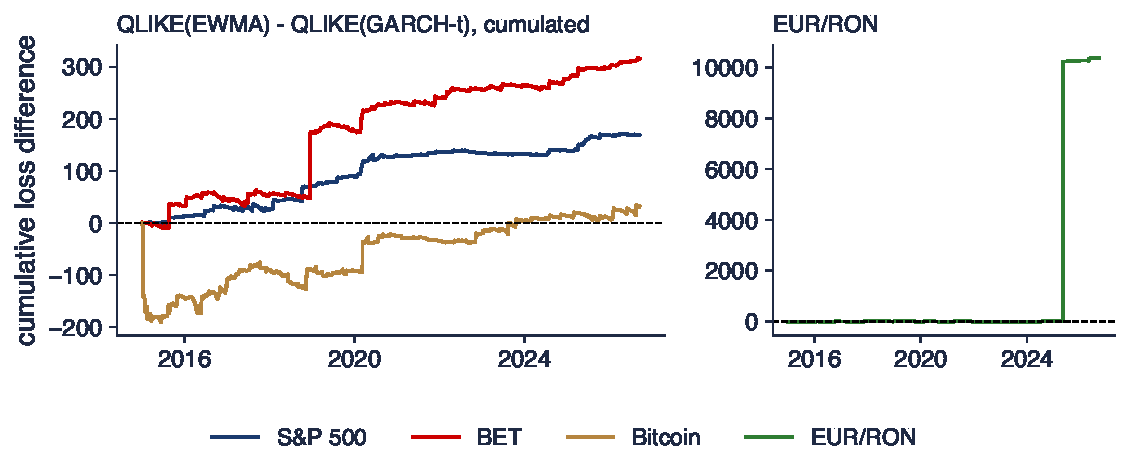
\includegraphics[width=0.97\textwidth,height=0.58\textheight,keepaspectratio]{tsa_ch5_forecast_eval.pdf}
\end{center}
\vspace{-0.25cm}
\begin{itemize}
    \item Prognoze ale varianței cu o zi înainte, din 2015 pînă la 18 septembrie 2026: GARCH(1,1)-t (reestimat la fiecare 250 de zile) față de EWMA cu $\lambda = 0{,}94$; o curbă crescătoare înseamnă că GARCH-t are QLIKE mai mic
\end{itemize}
\quantlet{TSA\_ch5\_forecasts}{\qlurl{TSA_ch5_forecasts}}
\end{frame}

\begin{frame}{Interpretarea comparației prognozelor}
\itemsize{\footnotesize}
\begin{center}
\scriptsize
\begin{tabular}{lrrrrr}
\toprule
2015--2026 & zile & QLIKE GARCH-t & QLIKE GJR-t & QLIKE EWMA & DM $t$, GARCH-t față de EWMA (p) \\
\midrule
S\&P 500 & 2\,944 & $0{,}761$ & $0{,}733$ & $0{,}819$ & ${\ensuremath{-}3{,}69}$ ($<$\,0{,}001) \\
BET & 2\,926 & $0{,}680$ & $0{,}674$ & $0{,}788$ & ${\ensuremath{-}2{,}22}$ (0{,}027) \\
EUR/RON & 2\,939 & $2{,}456$ & $3{,}276$ & $5{,}982$ & ${\ensuremath{-}1{,}02}$ (0{,}310) \\
Bitcoin & 4\,279 & $3{,}383$ & $3{,}401$ & $3{,}390$ & ${\ensuremath{-}0{,}20}$ (0{,}845) \\
\bottomrule
\end{tabular}
\end{center}
\begin{itemize}
    \item S\&P 500 și BET: GARCH-t este mai bun decît EWMA ($t < -1{,}96$); GJR-t are cel mai mic QLIKE (efectul de levier contează și în afara eșantionului)
    \item Bitcoin: nicio diferență ($t = \ensuremath{-}0{,}20$): GARCH-ul lui este un IGARCH, adică aproape un EWMA
    \item EUR/RON: QLIKE mediu mult mai mic pentru GARCH, dar $t = \ensuremath{-}1{,}02$: 98\% din diferența totală provine dintr-o singură zi, 6 mai 2025, cînd EWMA a prognozat o varianță aproape nulă
    \item Interpretare: QLIKE penalizează prognozele prea mici; testul DM ne ferește de concluzii construite pe o singură zi
\end{itemize}\quantlet{TSA\_ch5\_forecasts}{\qlurl{TSA_ch5_forecasts}}
\end{frame}

\begin{frame}{Studiu de caz: Hansen și Lunde (2005)}
\itemsize{\small}
\begin{itemize}
    \item \textbf{Întrebarea}: poate ceva să depășească un GARCH(1,1)? \refHL
    \begin{itemize}
        \item 330 de modele de tip ARCH (asimetrice, cu memorie lungă, cu inovații diferite), comparate în afara eșantionului pe cursul marcă germană/dolar american și pe randamentele unei acțiuni americane
        \item aproximarea: varianța realizată din randamente intrazilnice, mai precisă decît $r_t^2$
    \end{itemize}
    \item \textbf{Rezultatul}: la cursul de schimb, niciun model nu a depășit semnificativ GARCH(1,1); la acțiune, modelele cu efect de levier au fost mai bune
    \begin{itemize}
        \item același tipar ca în tabelul nostru: asimetria contează pentru acțiuni, nu pentru cursuri de schimb sau Bitcoin
    \end{itemize}
    \item \textbf{Moștenirea}: GARCH(1,1) este reperul pe care orice model nou de volatilitate, inclusiv de învățare automată (\tsachlink{https://danpele.github.io/Time-Series-Analysis/RO/Cursuri/capitol9_invatare_automata_serii_timp.pdf}{Capitolul 9}), trebuie să-l depășească în afara eșantionului
\end{itemize}
\end{frame}

\begin{frame}{Recapitulare: prognoza varianței}
\itemsize{\small}
\begin{itemize}
    \item $E_t[\sigma_{t+h}^2] = \bar\sigma^2 + (\alpha + \beta)^{h-1}(\sigma_{t+1}^2 - \bar\sigma^2)$; varianța pe $H$ zile = suma prognozelor zilnice
    \item Comparăm prognozele în afara eșantionului cu QLIKE și testul Diebold--Mariano
    \item GARCH este mai bun decît EWMA acolo unde volatilitatea revine la medie
\end{itemize}
\end{frame}


%=============================================================================
\section{O aplicație: VaR 1\% dintr-un model GARCH}
%=============================================================================

\begin{frame}{VaR condiționat}
\itemsize{\small}
\begin{itemize}
    \item \textbf{VaR} (value at risk, valoarea expusă la risc) la nivelul $\alpha$: pierderea depășită cu probabilitatea $\alpha$, $\mathrm{VaR}_\alpha = -q_\alpha(r_{t+1})$, unde $q_\alpha$ este cuantila de ordin $\alpha$
    \begin{itemize}
        \item aici $\alpha = 1\%$: VaR 1\%, o pierdere depășită într-o zi din o sută
    \end{itemize}
    \item Cu $r_{t+1} = \mu + \sigma_{t+1}z_{t+1}$: $\mathrm{VaR}_{t+1} = -(\mu + \sigma_{t+1}\,q_\alpha(z))$
    \begin{itemize}
        \item $q_\alpha(z)$: cuantila de ordin $\alpha$ a inovației $z$; Normală: $q_{0{,}01} = \ensuremath{-}2{,}326$
        \item t standardizată: $q_{0{,}01} = t_\nu^{-1}(0{,}01)\sqrt{(\nu - 2)/\nu}$, $t_\nu^{-1}$: funcția cuantilă a distribuției Student cu $\nu$ grade de libertate
        \item VaR se schimbă în fiecare zi odată cu $\sigma_{t+1}$: mare în furtuni, mic în perioadele liniștite
    \end{itemize}
    \item \textbf{Exemplu rezolvat}: S\&P 500 la 18 septembrie 2026, GARCH(1,1)-t: $\hat\mu = 0{,}079$, $\sigma_{t+1} = 0{,}714$, $\hat\nu = 6{,}26$
    \begin{itemize}
        \item $t_{\hat\nu}^{-1}(0{,}01) = \ensuremath{-}3{,}100$, $\sqrt{(\hat\nu - 2)/\hat\nu} = 0{,}825$, deci $q_{0{,}01} = \ensuremath{-}3{,}100 \times 0{,}825 = \ensuremath{-}2{,}557$
        \item VaR 1\% $= -(0{,}079 + 0{,}714 \times (\ensuremath{-}2{,}557)) = 1{,}75\%$
        \item cu $z_t$ Normale: $1{,}58\%$; pe 10 zile (suma varianțelor, fără $\mu$): $2{,}557 \times \sqrt{5{,}67} = 6{,}09\%$
    \end{itemize}
\end{itemize}
\end{frame}

\begin{frame}{VaR 1\% în timpul crahului COVID-19}
\itemsize{\footnotesize}
\begin{center}
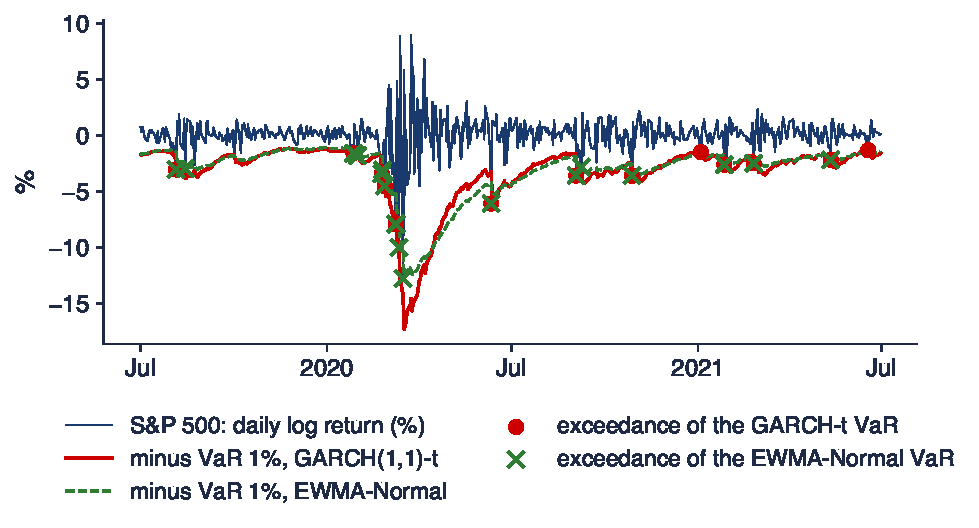
\includegraphics[width=0.97\textwidth,height=0.56\textheight,keepaspectratio]{tsa_ch5_var.pdf}
\end{center}
\vspace{-0.25cm}
\begin{itemize}
    \item S\&P 500, iulie 2019 -- iunie 2021 (505 zile): VaR 1\% pe o zi din GARCH(1,1)-t (reestimat la fiecare 250 de zile) și din EWMA cu $z_t$ Normale
    \item Depășiri (randament sub $-$VaR): GARCH-t 13, EWMA-Normal 17, circa 5 așteptate; ambele modele reacționează, dar abia după primele scăderi mari din martie 2020
\end{itemize}
\quantlet{TSA\_ch5\_forecasts}{\qlurl{TSA_ch5_forecasts}}
\end{frame}

\begin{frame}{Depășiri 2015--2026}
\itemsize{\footnotesize}
\begin{center}
\footnotesize
\begin{tabular}{lrrrr}
\toprule
VaR 1\% & zile & așteptat & GARCH-t & EWMA-Normal \\
\midrule
S\&P 500 & 2\,944 & 29 & 49 (1{,}66\%) & 65 (2{,}21\%) \\
BET & 2\,926 & 29 & 34 (1{,}16\%) & 67 (2{,}29\%) \\
EUR/RON & 2\,939 & 29 & 35 (1{,}19\%) & 63 (2{,}14\%) \\
Bitcoin & 4\,279 & 43 & 64 (1{,}50\%) & 93 (2{,}17\%) \\
\bottomrule
\end{tabular}
\end{center}
\begin{itemize}
    \item Un VaR 1\% corect este depășit în 1\% dintre zile, iar depășirile nu apar grupat
    \item EWMA-Normal: 2{,}1--2{,}3\% peste tot: cuantila Normală este prea mică pentru cozi groase
    \item GARCH-t: 1{,}2--1{,}7\%: mult mai aproape de 1\%; cel mai mare pentru S\&P 500, unde lipsește efectul de levier
    \item Sînt diferențele semnificative? Testul \refKupiec\ compară numărul de depășiri cu o distribuție binomială
\end{itemize}\quantlet{TSA\_ch5\_forecasts}{\qlurl{TSA_ch5_forecasts}}
\end{frame}

\begin{frame}{Recapitulare: VaR 1\% dintr-un model GARCH}
\itemsize{\small}
\begin{itemize}
    \item $\mathrm{VaR}_{t+1} = -(\mu + \sigma_{t+1}q_\alpha(z))$: o volatilitate dinamică și cuantila potrivită
    \item Cuantilele Normale subestimează riscul; Student-t este mult mai aproape de 1\%
    \item Mai multe serii deodată (covarianțele randamentelor): GARCH multivariat, \tsachlink{https://danpele.github.io/Time-Series-Analysis/RO/Cursuri/capitol14_modele_garch_multivariate.pdf}{Capitolul 14} (studiu individual)
\end{itemize}
\end{frame}


%=============================================================================
\section{Contribuția posibilă a AI}
%=============================================================================

\begin{frame}{Contribuția posibilă a AI}
\itemsize{\small}
\begin{itemize}
    \item \textbf{Cod}: o primă versiune a unui script care aplică ARCH-LM, estimează GARCH, GJR și EGARCH cu \texttt{arch} pe multe serii și tabelează rezultatele
    \item \textbf{Explicații}: o a doua explicație a formei ARMA(1,1) a modelului GARCH sau a unui tabel de rezultate \texttt{arch}
    \item \textbf{Explorare}: volatilitatea tuturor acțiunilor de la BVB sau a leului față de mai multe valute
    \item Exemplu de prompt
    \begin{itemize}
        \item \aiprompt{Write Python code that loads daily BET closes, computes log returns in percent, runs the ARCH-LM test with 5 lags, fits AR(1)-GARCH(1,1) with Student-t innovations using the arch package, and plots the annualised conditional volatility.}
    \end{itemize}
\end{itemize}
\end{frame}

\begin{frame}{Verificări necesare}
\itemsize{\small}
\begin{itemize}
    \item Unitățile: randamente în \%, nu în zecimale; rescalăm o serie cu varianță foarte mică (EUR/RON) și convertim înapoi $\omega$
    \item Persistența: $\alpha + \beta$ pentru GARCH, $\alpha + \beta + \gamma/2$ pentru GJR, $\beta$ pentru EGARCH
    \item Estimările pe frontieră ($\alpha + \beta = 1$): fără timp de înjumătățire și fără volatilitate de lungă durată; nu raportăm valori infinite
    \item Calendarele: Bitcoin se tranzacționează 7 zile pe săptămînă, BET cinci; anualizăm fiecare serie cu propria frecvență
    \item Prognozele în afara eșantionului folosesc doar date trecute; nivelul VaR se scrie VaR 1\%
    \item Fiecare referință citată: trebuie să existe; verificați DOI-ul
\end{itemize}
\end{frame}


%=============================================================================
\section{Rezumat}
%=============================================================================

\begin{frame}{Idei de reținut}
\itemsize{\small}
\begin{itemize}
    \item Randamentele: o medie aproape imprevizibilă și o varianță previzibilă, $r_t = \mu_t + \sigma_t z_t$; testăm cu ACF a lui $r_t^2$ și ARCH-LM
    \item GARCH(1,1) este un ARMA(1,1) pentru $\varepsilon_t^2$; $\alpha + \beta$ apropiat de 1; IGARCH și EWMA cînd $\alpha + \beta = 1$
    \item Estimăm prin verosimilitate maximă cu \texttt{arch} și raportăm SE robuste; inovații Student-t pentru cozi
    \item ARMA-GARCH: media din \tsachlink{https://danpele.github.io/Time-Series-Analysis/RO/Cursuri/capitol2_modele_arma.pdf}{Capitolul 2} și varianța din acest capitol, estimate împreună
    \item Indicii de acțiuni au nevoie de asimetrie (GJR, EGARCH); verificăm $\hat z_t$ și $\hat z_t^2$ după fiecare estimare
    \item Prognozele revin la nivelul de lungă durată; le comparăm în afara eșantionului cu QLIKE și DM; VaR 1\% $= -(\mu + \sigma_{t+1}q_{0{,}01}(z))$
\end{itemize}
\end{frame}

\begin{frame}{Formule de reținut}
\itemsize{\small}
{\renewcommand{\arraystretch}{1.4}\begin{center}
\scriptsize
\begin{tabular}{ll}
\toprule
\textbf{Mărimea} & \textbf{Formula} \\
\midrule
ARCH-LM & $\hat\varepsilon_t^2 = b_0 + \sum_{i=1}^{q}b_i\hat\varepsilon_{t-i}^2 + u_t$, \quad $\mathrm{LM} = nR^2 \sim \chi^2(q)$ \\
ARCH($q$) & $\sigma_t^2 = \omega + \sum_{i=1}^{q}\alpha_i\varepsilon_{t-i}^2$, \quad $\bar\sigma^2 = \omega/(1 - \sum\alpha_i)$ \\
GARCH(1,1) & $\sigma_t^2 = \omega + \alpha\varepsilon_{t-1}^2 + \beta\sigma_{t-1}^2$, \quad $\bar\sigma^2 = \omega/(1 - \alpha - \beta)$, \quad $h_{1/2} = \ln 0{,}5/\ln(\alpha + \beta)$ \\
EWMA & $\sigma_t^2 = \lambda\sigma_{t-1}^2 + (1 - \lambda)r_{t-1}^2$ \\
GJR, EGARCH & $\sigma_t^2 = \omega + (\alpha + \gamma I_{t-1})\varepsilon_{t-1}^2 + \beta\sigma_{t-1}^2$; \quad $\ln\sigma_t^2 = \omega + \alpha(|z_{t-1}| - E|z_{t-1}|) + \gamma z_{t-1} + \beta\ln\sigma_{t-1}^2$ \\
Log-verosimilitatea & $\ell = -\frac12\sum_t[\ln 2\pi + \ln\sigma_t^2 + (r_t - \mu_t)^2/\sigma_t^2]$ \\
Prognoza & $E_t[\sigma_{t+h}^2] = \bar\sigma^2 + (\alpha + \beta)^{h-1}(\sigma_{t+1}^2 - \bar\sigma^2)$ \\
QLIKE, VaR 1\% & $L = r_t^2/h_t + \ln h_t$; \quad $\mathrm{VaR}_{t+1} = -(\mu + \sigma_{t+1}\,q_{0{,}01}(z))$ \\
\bottomrule
\end{tabular}
\end{center}
}
\end{frame}

\begin{frame}{Autoevaluare}
\itemsize{\small}
\begin{itemize}
    \item \textbf{Întrebare}: $\omega = 0{,}05$, $\alpha = 0{,}05$, $\beta = 0{,}90$. Care sînt varianța de lungă durată și timpul de înjumătățire?
    \begin{itemize}
        \item \textbf{Răspuns}: $0{,}05/0{,}05 = 1$; $\ln 0{,}5/\ln 0{,}95 = 13{,}5$ zile
    \end{itemize}
    \item \textbf{Întrebare}: o regresie ARCH-LM cu $q = 5$ pe 1000 de reziduuri dă $R^2 = 0{,}004$. Există efecte ARCH la 5\%?
    \begin{itemize}
        \item \textbf{Răspuns}: nu: $\mathrm{LM} = 1000 \times 0{,}004 = 4 < 11{,}07$
    \end{itemize}
    \item \textbf{Întrebare}: GJR dă $\hat\alpha = 0$ și $\hat\gamma = 0{,}2$. Ce se întîmplă cu varianța după o creștere de 3\%?
    \begin{itemize}
        \item \textbf{Răspuns}: nimic în afară de scăderea $\beta\sigma_t^2$: doar șocurile negative cresc varianța
    \end{itemize}
    \item Urmează: \tsachlink{https://danpele.github.io/Time-Series-Analysis/RO/Cursuri/capitol6_modele_var_cauzalitate_granger.pdf}{Capitolul 6}, modele VAR și cauzalitate Granger (mai multe serii deodată)
\end{itemize}
\end{frame}


%=============================================================================
\section{Bibliografie}
%=============================================================================

\begin{frame}{Bibliografie (1/2)}
\itemsize{\tiny}
\begin{itemize}
    \item Akaike, H. (1974). A new look at the statistical model identification. \textit{IEEE Transactions on Automatic Control}, 19(6), 716--723. \href{https://doi.org/10.1109/TAC.1974.1100705}{doi:10.1109/TAC.1974.1100705}
    \item Andersen, T. G., \& Bollerslev, T. (1998). Answering the skeptics: Yes, standard volatility models do provide accurate forecasts. \textit{International Economic Review}, 39(4), 885--905. \href{https://doi.org/10.2307/2527343}{doi:10.2307/2527343}
    \item Bollerslev, T. (1986). Generalized autoregressive conditional heteroskedasticity. \textit{Journal of Econometrics}, 31(3), 307--327. \href{https://doi.org/10.1016/0304-4076(86)90063-1}{doi:10.1016/0304-4076(86)90063-1}
    \item Bollerslev, T. (1987). A conditionally heteroskedastic time series model for speculative prices and rates of return. \textit{Review of Economics and Statistics}, 69(3), 542--547. \href{https://doi.org/10.2307/1925546}{doi:10.2307/1925546}
    \item Bollerslev, T., \& Wooldridge, J. M. (1992). Quasi-maximum likelihood estimation and inference in dynamic models with time-varying covariances. \textit{Econometric Reviews}, 11(2), 143--172. \href{https://doi.org/10.1080/07474939208800229}{doi:10.1080/07474939208800229}
    \item Christie, A. A. (1982). The stochastic behavior of common stock variances: Value, leverage and interest rate effects. \textit{Journal of Financial Economics}, 10(4), 407--432. \href{https://doi.org/10.1016/0304-405X(82)90018-6}{doi:10.1016/0304-405X(82)90018-6}
    \item Diebold, F. X., \& Mariano, R. S. (1995). Comparing predictive accuracy. \textit{Journal of Business \& Economic Statistics}, 13(3), 253--263. \href{https://doi.org/10.1080/07350015.1995.10524599}{doi:10.1080/07350015.1995.10524599}
    \item Engle, R. F. (1982). Autoregressive conditional heteroscedasticity with estimates of the variance of United Kingdom inflation. \textit{Econometrica}, 50(4), 987--1007. \href{https://doi.org/10.2307/1912773}{doi:10.2307/1912773}
    \item Engle, R. F. (2004). Risk and volatility: Econometric models and financial practice. \textit{American Economic Review}, 94(3), 405--420. \href{https://doi.org/10.1257/0002828041464597}{doi:10.1257/0002828041464597}
    \item Engle, R. F., \& Bollerslev, T. (1986). Modelling the persistence of conditional variances. \textit{Econometric Reviews}, 5(1), 1--50. \href{https://doi.org/10.1080/07474938608800095}{doi:10.1080/07474938608800095}
    \item Engle, R. F., \& Ng, V. K. (1993). Measuring and testing the impact of news on volatility. \textit{Journal of Finance}, 48(5), 1749--1778. \href{https://doi.org/10.1111/j.1540-6261.1993.tb05127.x}{doi:10.1111/j.1540-6261.1993.tb05127.x}
    \item Franke, J., Härdle, W. K., \& Hafner, C. M. (2019). \textit{Statistics of Financial Markets: An Introduction} (5th ed.). Springer. \href{https://doi.org/10.1007/978-3-030-13751-9}{doi:10.1007/978-3-030-13751-9}
    \item Glosten, L. R., Jagannathan, R., \& Runkle, D. E. (1993). On the relation between the expected value and the volatility of the nominal excess return on stocks. \textit{Journal of Finance}, 48(5), 1779--1801. \href{https://doi.org/10.1111/j.1540-6261.1993.tb05128.x}{doi:10.1111/j.1540-6261.1993.tb05128.x}
    \item Hamilton, J. D. (1994). \textit{Time Series Analysis}. Princeton University Press. \href{https://doi.org/10.2307/j.ctv14jx6sm}{doi:10.2307/j.ctv14jx6sm}
    \item Hansen, B. E. (1994). Autoregressive conditional density estimation. \textit{International Economic Review}, 35(3), 705--730. \href{https://doi.org/10.2307/2527081}{doi:10.2307/2527081}
    \item Hansen, P. R., \& Lunde, A. (2005). A forecast comparison of volatility models: Does anything beat a GARCH(1,1)? \textit{Journal of Applied Econometrics}, 20(7), 873--889. \href{https://doi.org/10.1002/jae.800}{doi:10.1002/jae.800}
\end{itemize}
\end{frame}

\begin{frame}{Bibliografie (2/2)}
\itemsize{\tiny}
\begin{itemize}
    \item Huang, C., \& Petukhina, A. (2022). \textit{Applied Time Series Analysis and Forecasting with Python}. Springer. \href{https://doi.org/10.1007/978-3-031-13584-2}{doi:10.1007/978-3-031-13584-2}
    \item Hyndman, R. J., \& Athanasopoulos, G. (2021). \textit{Forecasting: Principles and Practice} (3rd ed.). OTexts. \href{https://otexts.com/fpp3/}{otexts.com/fpp3}
    \item J.P. Morgan/Reuters (1996). \textit{RiskMetrics -- Technical Document} (4th ed.). Morgan Guaranty Trust Company. \href{https://www.msci.com/documents/10199/5915b101-4206-4ba0-aee2-3449d5c7e95a}{msci.com}
    \item Kupiec, P. H. (1995). Techniques for verifying the accuracy of risk measurement models. \textit{Journal of Derivatives}, 3(2), 73--84. \href{https://doi.org/10.3905/jod.1995.407942}{doi:10.3905/jod.1995.407942}
    \item Ljung, G. M., \& Box, G. E. P. (1978). On a measure of lack of fit in time series models. \textit{Biometrika}, 65(2), 297--303. \href{https://doi.org/10.1093/biomet/65.2.297}{doi:10.1093/biomet/65.2.297}
    \item Mandelbrot, B. (1963). The variation of certain speculative prices. \textit{Journal of Business}, 36(4), 394--419. \href{https://doi.org/10.1086/294632}{doi:10.1086/294632}
    \item McLeod, A. I., \& Li, W. K. (1983). Diagnostic checking ARMA time series models using squared-residual autocorrelations. \textit{Journal of Time Series Analysis}, 4(4), 269--273. \href{https://doi.org/10.1111/j.1467-9892.1983.tb00373.x}{doi:10.1111/j.1467-9892.1983.tb00373.x}
    \item Nelson, D. B. (1991). Conditional heteroskedasticity in asset returns: A new approach. \textit{Econometrica}, 59(2), 347--370. \href{https://doi.org/10.2307/2938260}{doi:10.2307/2938260}
    \item Patton, A. J. (2011). Volatility forecast comparison using imperfect volatility proxies. \textit{Journal of Econometrics}, 160(1), 246--256. \href{https://doi.org/10.1016/j.jeconom.2010.03.034}{doi:10.1016/j.jeconom.2010.03.034}
    \item Schwarz, G. (1978). Estimating the dimension of a model. \textit{Annals of Statistics}, 6(2), 461--464. \href{https://doi.org/10.1214/aos/1176344136}{doi:10.1214/aos/1176344136}
    \item Tsay, R. S. (2010). \textit{Analysis of Financial Time Series} (3rd ed.). Wiley. \href{https://doi.org/10.1002/9780470644560}{doi:10.1002/9780470644560}
\end{itemize}
\end{frame}

\end{document}
